\documentclass[letterpaper,10pt]{article}
\usepackage[backend=biber,style=numeric,sorting=none]{biblatex}
\bibliography{refrences}
\usepackage[utf8]{inputenc}
\usepackage{t1enc}
\usepackage{appendix}
\usepackage{graphicx}
\usepackage{wrapfig}
\usepackage{xcolor}
\usepackage{color}
\usepackage{epsfig}
\usepackage{pdflscape}
\usepackage{color,soul}
\usepackage{pdfpages}
\usepackage{verbatim}
\usepackage{xcolor,colortbl}
\usepackage{gensymb}
\usepackage[final]{pdfpages}
\usepackage[nottoc]{tocbibind}
\usepackage{setspace}
\usepackage{caption}
\usepackage{float}
\usepackage{epigraph}
\graphicspath{ {images/} }
\renewcommand{\baselinestretch}{1}
\setlength{\textheight}{9in}
\setlength{\textwidth}{6.5in}
\setlength{\headheight}{0in}
\setlength{\headsep}{0in}
\setlength{\topmargin}{0in}
\setlength{\oddsidemargin}{0in}
\setlength{\evensidemargin}{0in}
\setlength{\parindent}{.3in}
\usepackage{tocloft}
\usepackage{chngcntr}
\setcounter{secnumdepth}{4} % changes the depth of the subsection numberings
\counterwithin{figure}{section}
\counterwithin{table}{section}
\usepackage[usenames, dvipsnames]{color}
\definecolor{myblue}{RGB}{51,110,170}

\usepackage[toc,page]{appendix}

\usepackage{array}
\newcolumntype{L}{>{\arraybackslash}m{8cm}}

\let\oldsection\section
\let\oldsubsection\subsection
\renewcommand{\section}{\def\cursectioning{section}\oldsection}
\renewcommand{\subsection}{\def\cursectioning{subsection}\oldsubsection}

\newcounter{seccounter}[subsection]
\renewcommand{\theseccounter}{\csname the\cursectioning\endcsname.\arabic{seccounter}}

\newcommand{\Counter}{\stepcounter{seccounter}\theseccounter}


\setlength{\parindent}{2em}
\setlength{\parskip}{0.5em}


\setlength\epigraphwidth{15cm}
\setlength\epigraphrule{0pt}



\renewcommand\cfttoctitlefont{\hfill\Large\uppercase}
\renewcommand\cftaftertoctitle{\hfill\mbox{}}

\renewcommand\cftloftitlefont{\centering\Large\uppercase}
\renewcommand\cftlottitlefont{\centering\Large\uppercase}



\begin{document}
\pagestyle{empty}
\pagenumbering{roman}

\addtocontents{toc}{\vskip 1.5cm}
\addtocontents{lof}{\vskip 1.5cm}
\addtocontents{lot}{\vskip 1.5cm}

\begin{center}
\doublespacing
\vspace{30mm}
\uppercase{\Large{Electrophysiological solutions on smart \\ devices for Autistic, ADHD, locked-in syndrome patients and drowsy drivers}}
\vspace{8mm}

\normalsize{A Thesis Project
Submitted to the ESTEEM Program\\
at the University of Notre Dame
in Partial Fulfillment of the Requirements\\
for the Degree of \\}
\vspace{8mm}
\doublespacing
\large{Master of Science}\\
by\\
\textbf{Kunigunda Szentes}\\%KUNIGUNDA SZENTES
\end{center}
\vspace{5mm}

\begin{flushright}
\hspace{0.3in}\noindent\rule{7cm}{0.4pt}
\end{flushright}
\rightline{András Horváth, Ph.D., Technical Adviser}
\vspace{4mm}

\begin{flushright}
\hspace{0.3in}\noindent\rule{7cm}{0.4pt}
\end{flushright}
\rightline{Tamás Králik (Mindtech), Technical Adviser}
\vspace{4mm}

\begin{flushright}
\hspace{0.3in}\noindent\rule{7cm}{0.4pt}
\end{flushright}
\rightline{Sunny Shah, Ph.D., ESTEEM Adviser}
\vspace{4mm}

\begin{flushright}
\hspace{0.3in}\noindent\rule{7cm}{0.4pt}
\end{flushright}
\rightline{Sam Miller, Business Adviser}
\vspace{4mm}


\begin{flushright}
\hspace{0.3in}\noindent\rule{7cm}{0.4pt}
\end{flushright}
\rightline{Kristóf Iván, Ph.D., Technical Adviser}
\vspace{4mm}

\vfill
\begin{center}
Engineering, Science, and Technology Entrepreneurship Excellence Master's Program\\
Notre Dame, Indiana\\
May 2018\\
\end{center}
\onehalfspacing
\pagebreak
\pagestyle{plain}

\hspace{0pt}
\vfill
\begin{center}
\uppercase{\Large{Confidentiality notice}} \\
\vspace{10mm}
\normalsize{This document is proprietary and confidential. No part of this document may be disclosed in any manner to a third party without the prior written consent of Mindtech.}
\end{center}
\vfill
\hspace{0pt}
\pagebreak


\vspace{100mm}
\begin{center}
\uppercase{\Large{Executive Summary\\}}
\addcontentsline{toc}{section}{Executive Summary}
\vspace{5mm}
\Large{\textit{Electrophysiological solutions on smart \\ devices for ADHD, locked-in syndrome patients and drowsy drivers\\}}
\vspace{5mm}
\normalsize{by\\}
\vspace{5mm}
\normalsize{Kunigunda Szentes\\}
\vspace{15mm}
\end{center}

\begin{onehalfspace}

\large{\bf{Problem}}

The number of students ages 6-21 with disabilities rose to 5.83 million in 2014, and this number is continuously rising. More and more children suffer from attention problems, which is one of the cognitive symptoms of diseases like Attention Deficit Hyperactivity Disorder (ADHD), Down syndrome, Obsessive-Compulsive Disorder (OCD), Autism spectrum disorder, and Rett syndrome. The number of affected students has increased dramatically over the past 10 years. Some of these cases, for example in a severe case of Autism spectrum disorder, children are nonverbal and thus cannot give any feedback about their level of engagement to the professionals working with them. The information about their preferences, interests, level of attention and engagement would help the therapists find the most effective method of educational methods. Teachers working in the field of special education could utilize statistics about the attention spans of their students for building a better curriculum, providing data driven reports for parents, colleagues, and other stakeholders.

\large{\bf{Product}}


Technology will continue to transform special education classroom instruction by enhancing individual learning opportunities and enabling greater flexibility and personalization. Mindtech offers a brain monitoring application in the special education market for teachers who frequently interact with these students, especially in the nonverbal cases.
Mindtech choose to use the NeuroSky Mindwave Mobile headset to collect real time brain wave data from its users. It combines this technology with Android/iOS development and all the applications coming from this process are accessible for devices from smart phones to tablets. All these features - with this practical EEG measuring headset - make Mindtech's technology portable, flexible and easily spreadable.

\large{\bf{Target market}}

The number of students ages 6-21 with disabilities fell to a low of 5.67 million in the fall of 2011, but rose to 5.83 million by the fall of 2014, the most recent year for which statistics are available. The past two years have seen an uptick, however, driven by students identified as having autism or “other health impairments.” The count had risen to 5.83 million by fall 2014, the most recent year for which statistics are available. 
The target market is the 13,299 special schools in the US, either private or public, which work with children with learning disabilities. 

\large{\bf{Competitive advantage}}

Mindtech identifies the best rehabilitation practice for each individual by utilizing real time brainwave data in the most affordable way. The system consists of a NeuroSky EEG headset and a smartphone with the Mindtech application, as well as an online platform where the data processing and visualization can occur. Mindtech helps trainers find the best rehabilitation and education practices. Special education trainers perform various training tasks and the software processes the patient's brainwaves and finds the task that caused the highest increase in attention level. As of now, there is no other application running on smart devices that can perform the same measure, connected to an online data storing and processing platform. 

The data storage of the application is cloud based. Currently, the algorithms are based on statistical methods, but in the future, advanced data analysis will be implemented based on artificial intelligence.


\end{onehalfspace}


\newpage
\tableofcontents

\newpage
\listoffigures
\newpage
\listoftables

\newpage
\vspace{70mm}
\begin{center}

\uppercase{\Large{Abbreviations}}
\addcontentsline{toc}{section}{Abbreviations}

\vspace{20mm}
\end{center}

\noindent ADHD - Attention Deficit Hyperactivity Disorder \\
AC -  Alternating Current \\
A/D - Analog to Digital Conversion \\
ALS - Amyotrophic Lateral Sclerosis \\
BCI - Brain Computer Interface \\
BMC - Business Model Canvas \\
B2B - Business to Business \\
B2C - Business to Customer \\
DMS - Driver Monitoring system \\
DSM - Diagnostic and Statistical Manual of Mental Disorders \\
EBITDA - Earnings before interest, taxation, depreciation and amortization \\
ECoG - Electrocorticography \\
EEG - Electroencephalography \\
EULA - End-User License Agreement \\
fMRI - Functional Magnetic Resonance Imaging \\
GUI - Graphical User Interface \\
iOS - Mobile operating system developed by Apple corp \\
IDEA - Individuals with Disabilities Education Act \\
IP - Intellectual Property \\
LIS - Locked-In Syndrome \\ 
LLC - Limited Liability Company \\
NSF - National Sleep Foundation \\
OCD - Obsessive-Compulsive Disorder \\
OEM - Original Equipment Manufacturer  \\
OSEP - Office of Special Education Programs \\
SaaS - Software as a Service \\
SDK - Software Development Kit \\
SWOT - Strengths, Weaknesses, Opportunities, Threats \\
TGAM - ThinkGear ASIC Module \\
TGAT -ThinkGear ASIC Chip \\
UI - User Interface \\
US - United States \\
USPTO - United States Patent and Trademark Office \\

\onehalfspacing
\newpage

\pagebreak
\begin{comment}
\vspace{70mm}
\begin{center}

\uppercase{\Large{Acknowledgements}}
\addcontentsline{toc}{section}{Acknowledgements}

\vspace{20mm}
\end{center}

Pazmany (Kristofok, adminisztracio), Esteem, Mindtech, Nora, csalad, Ornella, Tim 
\onehalfspacing
\end{comment}
\newpage

%%%%%%%%%%%%%%%%%%%%%%%%%%%%%%%%%%%%%% CH 1 %%%%%%%%%%%%%%%%%%%%%%%%%%%%%%%%%%%%%%%%%%

\pagenumbering{arabic} 
\vspace{100mm}
\begin{center}
\uppercase{\Large{Chapter 1}}
\section{\uppercase{\large{NEUROLOGICAL DISORDERS AND DRIVER ALERTNESS MARKET OVERVIEW}}}
%\addcontentsline{toc}{section}{Chapter 1: Problem statement and market analysis}
%\section[Chapter 1: Overview and objectives]{\uppercase{\large{Overview and objectives}}}
\vspace{20mm}
\end{center}
%\setcounter{section}{1}

\subsection{Problem statement}

Several mental disorders lead to a state, where patients cannot properly interact with their environment. For example patients suffering from specific types of transient or permanent paralysis, Locked in Syndrome or ALS, are nearly unable get on without external help, which, in most cases leads to cognitive impairment, anxiety, and/or depression. Moreover, nowadays more and more children suffer from  attention problems which is one of the cognitive symptoms of  diseases like ADHD (Attention Deficit Hyperactivity Disorder), Down syndrome, OCD (Obsessive-Compulsive Disorder), Autism spectrum disorder, and Rett syndrome. These children cannot give any feedback about their attention level to the professionals working with them, although that information would help the therapists find the most effective method of treatment.
Viewing from a different angle, giving ourselves feedback about our own attention level can be hard, in case of a long car ride. Some drivers do not recognize the point when they should stop  for a break. 
In summary, all the above mentioned problems are related to cognitive functions, which should be measured in the everyday life.


\subsection{ADHD syndrome}

\subsubsection{Diagnosis}

Attention deficit hyperactivity disorder is one of the most common mental health disorders of childhood, with prevalence rates ranging from 2\% to 9\%, based on information from the American Academy of Child and Adolescent Psychiatry. \cite{pelham_fabiano_massetti_2005} 

We can differentiate three main subtypes of ADHD: \cite{market_ADHD}
\begin{itemize}
\item \textbf{Combined Type}: involves the combined characteristics of hyperactivity, impulsiveness and inattention
\item \textbf{Predominantly Inattentive Type}: with inattention as the primary characteristic
\item \textbf{Predominantly Hyperactive-Impulsive Type}: with hyperactivity and impulsiveness as primary characteristics
\end{itemize}

Diagnostic criteria for ADHD in the case of a Predominantly Inattentive Presentation includes the following symptoms consistently occurring for minimum half a year, based on the DSM-5 system: "the child often fails to give close attention to details or makes careless mistakes in schoolwork, other activities; the child often does not seem to listen when spoken to directly; the child often does not follow through on instructions and fails to finish school work, duties;  the child is often easily distracted by extraneous stimuli; the child is often forgetful in daily activities." \cite{diagnostic_criteria_adhd} Some co-existing conditions include: learning disabilities, anxiety disorder, depression, in form of comorbid disorders. Comorbidity in ADHD appears up to 66 \% of the clinically referred children. \cite{market_ADHD}

These difficulties continue to occur in adolescence and adulthood, even though core symptoms may improve with age.  \cite{pelham_fabiano_massetti_2005} The causes and risk factors for ADHD are still unknown, but current research shows that genetics plays an important role. In addition to genetics, scientists are studying other possible causes and risk factors including alcohol and tobacco use during pregnancy and premature delivery. \cite{adhd_general}

\subsubsection{Statistics about ADHD}

\paragraph{Affected children and adults}

The percent of children estimated to have ADHD has changed over time and varying by the way it is measured. The Centers for Disease Control and Prevention (CDC) said in 2014 that 11\% of American children, ages 4 to 17, have the attention disorder (\~{} 7 million).  That’s an increase of 42 \% in just eight years. ADHD isn’t just a childhood disorder, about 4 \% of American adults over the age of 18 deal with ADHD on a daily basis (\~{} 5 million). There are demographic factors that impact the risks of ADHD diagnosis: a children living in households that make less than two times the federal poverty level, are in higher risk than childs born in higher-income households. \cite{healthline_adhd} We can see the illustration of the statistics on Figure \ref{fig:stat}, as well as the distribution of the possible presentations. Moreover we can see prevalence of children affected by ADHD by state on Figure \ref{fig:adhd_map}. As the legend indicates, the dark blue areas, for example Illinois, Indiana, Michigan, are the most affected.

\vspace{4mm}
\begin{figure}[h]
\centering
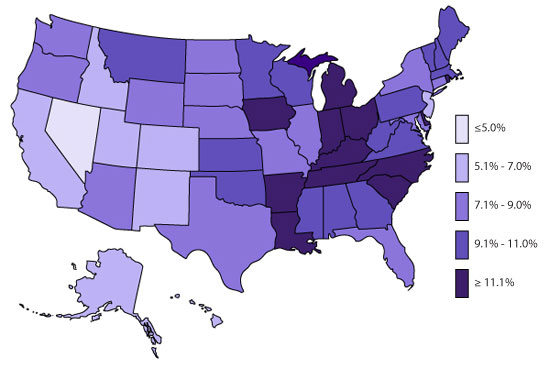
\includegraphics[scale=0.5]{map.jpg}
\caption[Percent of Youth Aged 4-17 with Attention-Deficit/Hyperactivity Disorder by State]{Percent of Youth Aged 4-17 with Attention-Deficit/Hyperactivity Disorder by State, \textit{National Survey of Children's Health, 2011}}
\label{fig:adhd_map}
\end{figure}


\vspace{4mm}
\begin{figure}[h]
\centering
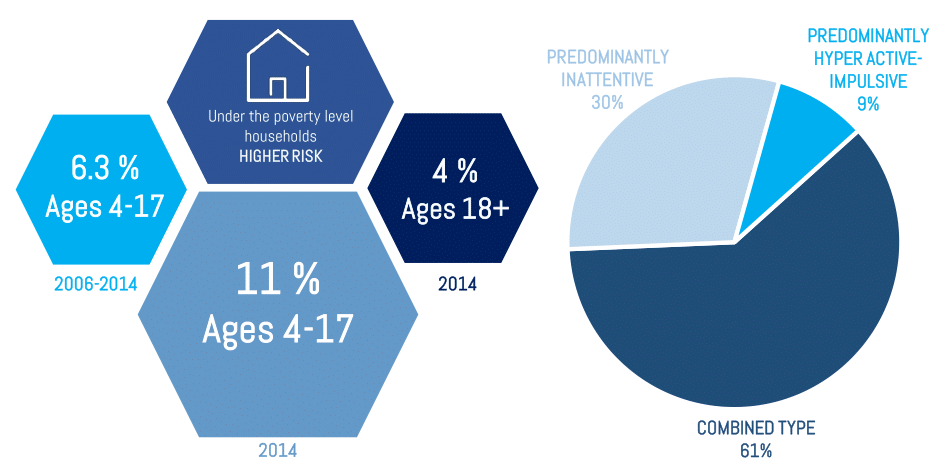
\includegraphics[scale=0.3]{diagnosis.png}
\caption[General statistics about ADHD affected children and adults in the United States]{General statistics about ADHD affected children and adults in the United States. \textit{Centers for Disease Control and Prevention | American Academy of Child \& Adolescent Psychology}}
\label{fig:stat}
\end{figure}


\paragraph{Cost of illness}
A study from 2007 claimed that the “cost of illness” for a person with ADHD is \$14,576 each year. Therefore ADHD costs Americans \$42.5 billion dollars each year — and that’s on the conservative side of ADHD prevalence estimates. Since the impairment in attention may lead to difficulty with academic achievement, inattentiveness and the disease is often combined with trauma, anxiety, the impact of the disease can be broader. Besides medication expenses, the costs of ADHD include education expenses and health care costs, loss of work and juvenile justice. \cite{healthline_adhd}
On Figure \ref{fig:adhd_cost} we can see the estimated annual direct costs of ADHD (\$1,574 million) as well as the amount of money spent on payments (\$2,728 million) related to ADHD. Moreover we can see the break-up of direct and indirect costs in detail: health care costs (\$12.2 billion), treatment of patients (\$1.6 billion), costs related to work loss for adults (\$3.7 billion), heath care costs of family members with ADHD (\$14.2 billion).

We can conclude that ADHD is associated with a significant financial and emotional costs to health care systems, educational services, primary caretakers and families, and overall society as a whole. Providing effective treatment will improve the quality of life of individuals with ADHD, their carers and families, and at the same time will reduce the financial implications and psychological burden of ADHD to society. \cite{adhd_book}

\vspace{4mm}
\begin{figure}[h]
\centering
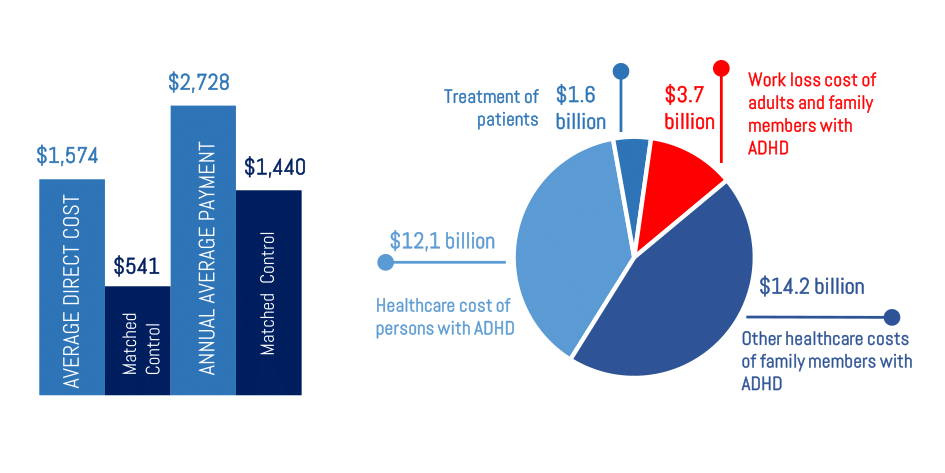
\includegraphics[scale=0.3]{cost.png}
\caption[Estimated cost of ADHD]{Estimated cost of ADHD covering treatment costs, other healthcare costs for both patient and their family members \textit{Department of Psychology, Center for Children and Families, State University of New York at Buffalo}\cite{cost}}
\label{fig:adhd_cost}
\end{figure}

Unfortunately there are a lot of negative statistics involving adolescents suffering from ADHD, such as lowered academic outcomes, social problems, and juvenile justice interaction the system. Figure \ref{fig:adhdnegstat} summarizes the biggest problems related to ADHD: patients are more likely to use drugs or alcohol, having more interpersonal problems and juvenile justice controlled cases.

\vspace{4mm}
\begin{figure}[h]
\centering
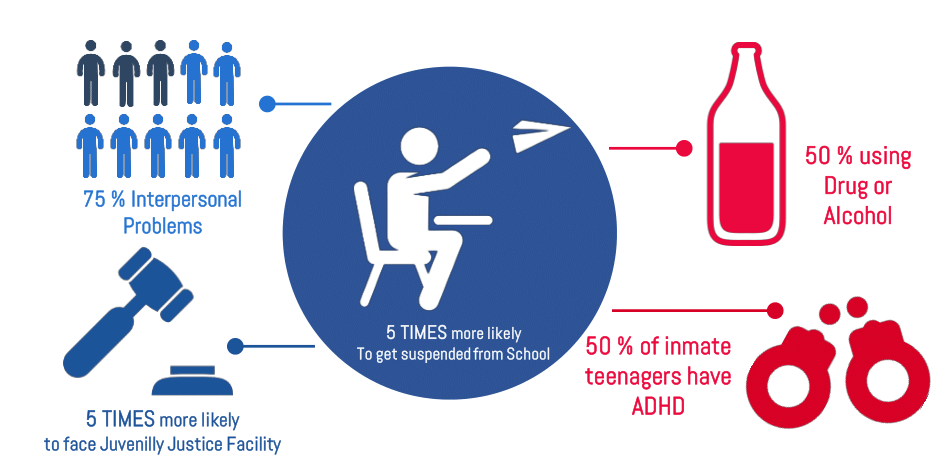
\includegraphics[scale=0.3]{sideff.png}
\caption[Negative outcome statistics in case of teenagers suffering from ADHD ]{Negative outcome statistics in case of teenagers suffering from ADHD, \textit{Center for Disease Control and Prevention 2016}}
\label{fig:adhdnegstat}
\end{figure}

\subsubsection{Current resources for ADHD treatment's}

\paragraph{Medications}

Medication treatment is only effective in managing the everyday symptoms and it can help children with ADHD in their everyday life. Stimulant-based medications are the best-known and most widely used ADHD medications. Their efficiency is clear, 70-80 \% of the children with ADHD have fewer symptoms when taking these fast-acting medications. However each medication affects each child differently; not every child responds well to medication. It is important that the primary caretaker and the practitioner work together to find the ideal medication and dose, based on the child's reactions. \cite{adhd_general} However, the use of medications is really divisive among parents and many parents try to avoid this solution.

Symptoms of ADHD typically first appear between the ages of 3 and 6. Currently, 6.1 \% of all American children are being treated for ADHD with medication. Some states have higher rates of treatment with medication than others. \cite{healthline_adhd}
The percent of children 4-17 years of age taking ADHD medication increased from 4.8 \% in 2007 to 6.1 \% in 2011. Among children with special health care needs, 9 out of 10 children with ADHD were receiving treatment: 43\% were treated with medication alone and 13 \% received behavioral therapy alone. \cite{adhd_general}


\paragraph{Psycho-Social Trainings} 

Primary literature shows that behavior therapy is an important part of treatment for children with ADHD. The disease affects not only a child’s ability to pay attention, or behave well at school, it also affects relationships with family and other children. 

In the case of behavior therapy with children, the therapist works with the children suffering from ADHD to learn new behaviors in order to replace behaviors that cause problems. In parent training in behavior therapy, parents learn skills to teach and lead their children to better behaviors.\cite{adhd_general} Behavioral class interventions are conducted by a teacher; they are interacting with the children to reach the same result. This technique works well with young children, although it is not effective with older childs.

The social impairments become more  dominant during  adolescence. This is the time when the teenagers get  their drivers licences, which can be very dangerous in an inattentive presentation. Besides the high-risky driving behaviors, social and academic failures, or even jail can be a side effect of this problem. Since teenagers have less oversight from parents and teachers, compared to middle school students, it is almost impossible to conduct behavior therapies. 

\paragraph{Neurofeedback Trainings} \\

Neurofeedback and cognitive trainings aim to develop working memory, attention, executive functioning and organization skills. \cite{pelham_fabiano_2008} These trainings are usually happen during a one-to-one appointment with a school psychologist or a private therapist. There are several computer softwares for cognitive function improvement. These sessions can show demonstrable progress in a specific sterile office environment, but fail to transfer into the classroom environment, where we would expect the actual results to occur.
The lack of trasfer can be explained with the phenomenon. There is a difference between the child's skill and performance. In case of a skill deficit (which the neurofeedback training is aiming to treat) the child is not aware of the right behavior, so he or she demonstrate the correct behavior in the class environment. However, in case of a performance deficit, the child has already gained the skill of the right behavior, but cannot conduct it in the actual situation. 

Since both the family and psychologist is seek a fully succesful outcome, and results from the training, not for partial success achieved during cognitive trainings, a many researchers do not support the effectiveness of these methods. However, as I mentioned in the previous paragraph, in case of adolescents the success of behavior therapies are considered as big as challenge  as the one-to-one training sessions.

Another problem regarding ADHD treatments is the lack of accessibility of behavioral trainings as professionals are in most cases unreachable from both a financial and geographic point of view. If the parents and teachers in school, or even the child itself could be able to take control over its case, providing a way of improving academic performance, a big impact could be created in ADHD treatment. Neurofeedback has not been tested at large; we have only opinions based on literature studies and isolated cases from one-on-one sessions with professionals. Furthermore neurofeedback already shows positive effects when combined with medication, especially in studies of performance-related scenarios.

To provide an overview of the process from diagnosis, to treatment, Figure \ref{fig:adhdstake} presents the main players of the process and the level of their influence as well.



\vspace{4mm}
\begin{figure}[h]
\centering
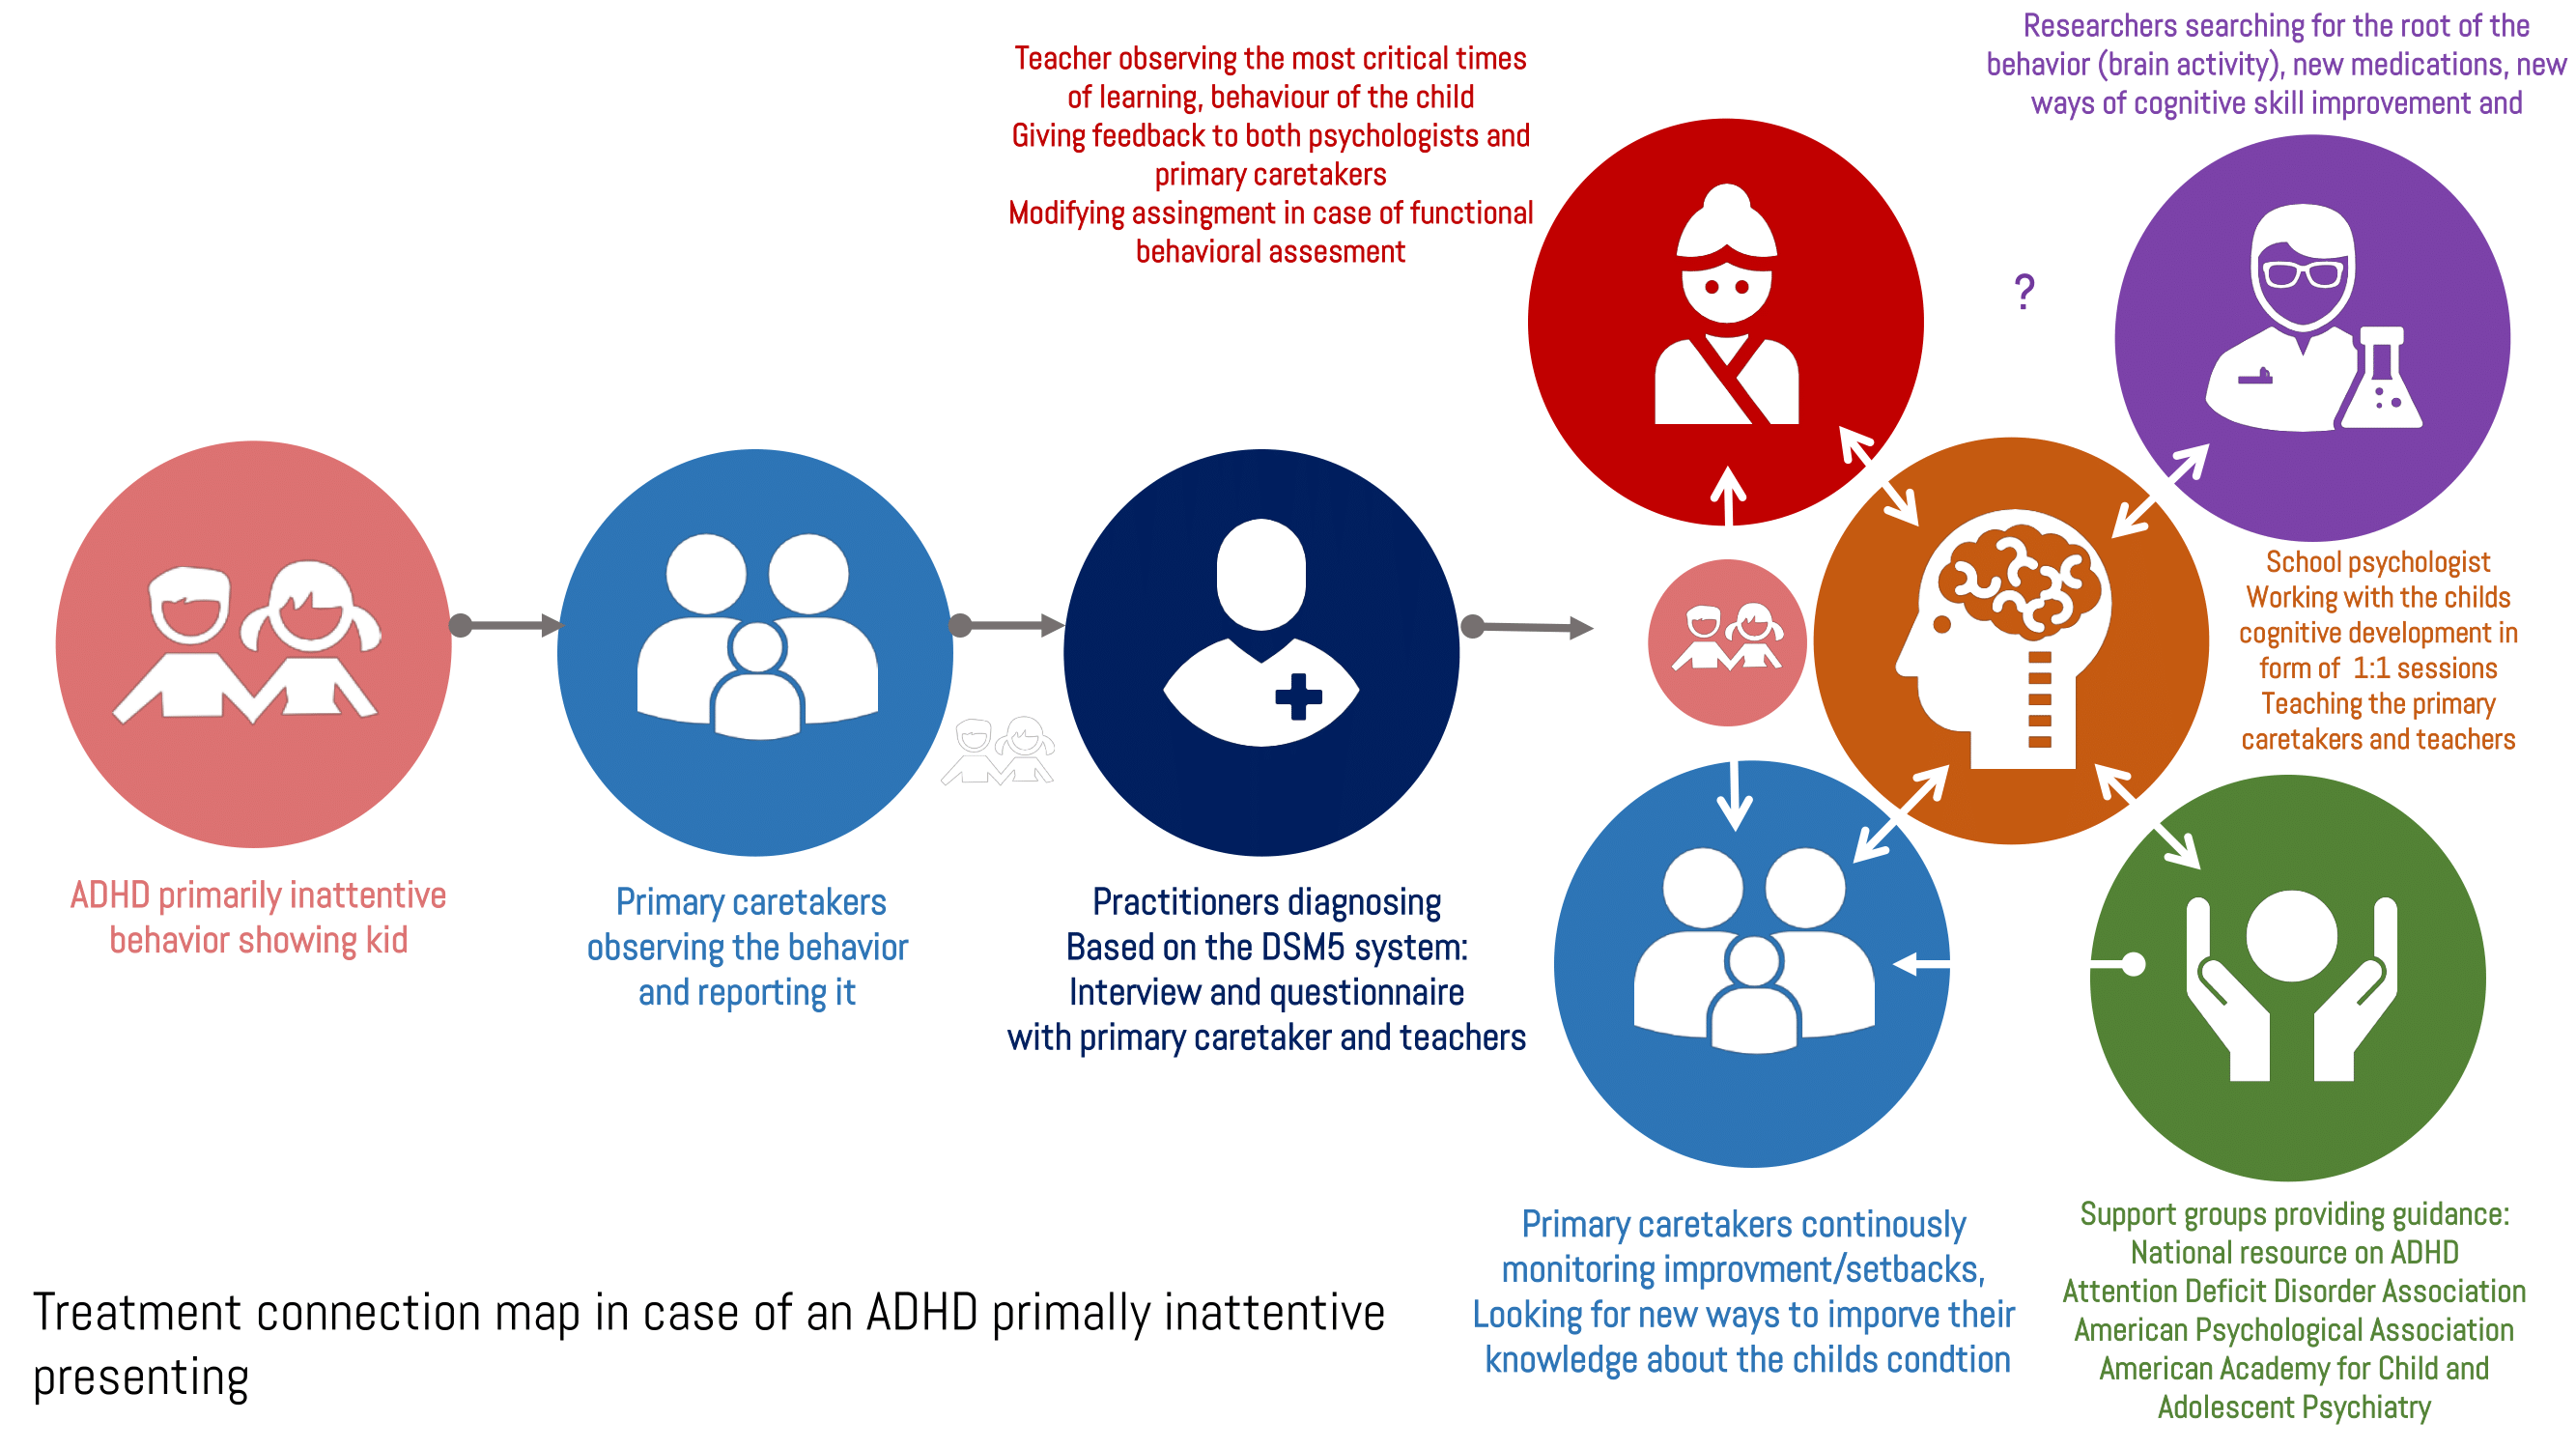
\includegraphics[scale=0.17]{treatment.png}
\caption{The flowchart presenting the key players through process of ADHD diagnosis to the treatment methods}
\label{fig:adhdstake}
\end{figure}


In summary, medications are mostly target symptoms while psycho-Social trainings and cognitive trainings are targeting both symptoms and impairments. The overview of the usage of different treatment usage around the United States is visualized in the following figure \ref{fig:maptreat}.

\vspace{4mm}
\begin{figure}[h]
\centering
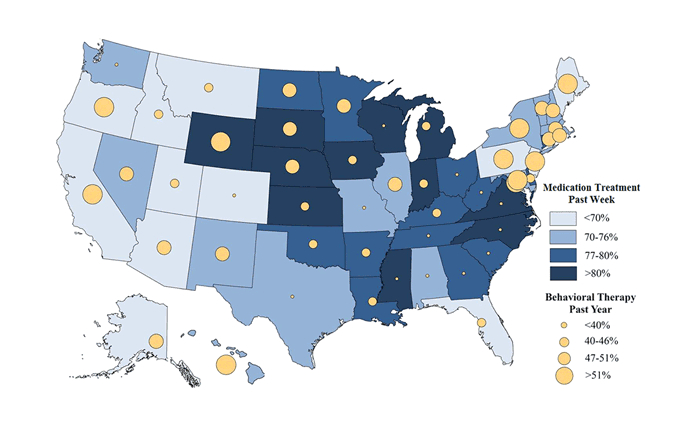
\includegraphics[scale=0.5]{map-med.jpg}
\caption[ADHD medication and behavior therapy among children with ADHD (ages 4-17) with special health care needs]{ADHD medication and behavior therapy among children with ADHD (ages 4-17) with special health care needs \textit{National Survey of Children's Health, 2011}}
\label{fig:maptreat}
\end{figure}

\subsubsection{Market analysis for ADHD syndrome solutions}
\paragraph{Market size}

\subparagraph{Total available market} It is estimated that around 11 \% of American children, from age 4 - 17 are diagnosed with ADHD. Furthermore, almost 50 \% of these children are carry symptoms to adulthood. Moreover around 4 \% of adults have ADHD in the US, which makes approximately 12 million people in America affected with ADHD. \cite{market_ADHD}

\subparagraph{Served market} Only around 48 \% of the estimated 4 million Americans childs and children affected by ADHD are currently treated for this condition, which makes 2.02 million child or adolescent receiving any treatment (medication or therapy). Additionally, 0.6 million adults are treated, therefore 2.62 million patients currently receive any kind of ADHD treatment. \cite{market_ADHD} It is straightforward to say that we can only serve the people already receiving a treatment, although with Mindtech's solution is not impossible to reach customers who are currently not within this segment. All in all, this 2.62 million can be a bigger number if Mindtech proves to be accessible enough from a financial point of view. 

\subparagraph{Target market} 
The primary inattentive presentation affects 30 \% , whilst the combined type affects an estimated 61 \% of the 2.6 million children, adolescents and adults in the US. In total, Mindtech can provide a valuable training experience for 2.18 million people diagnosed with ADHD. From this number it is logical to exclude the people who only believe in medications. For the ones who already experience that therapy is a very good complement to any medication, Mindtech's solution can be extremely valuable because it is affordable and location independent. 
The main target of the Mindtech solution is children, adolescents and young adults who are lack the financial support for continuous therapy sessions and aim to increase their study performance. In case of  children, the main targets are the parents aiming to contribute more in their children's school performance. In the case of adolescents and young adults, our main target are the users themselves, and the schools and universities aiming to help the academic performance of the students diagnosed with ADHD, by providing appropriate resources. 

\paragraph{Market segmentation}

The market can be divided in two main parts:
\begin{itemize}
\item B2C:  patients diagnosed with ADHD  and their primary caretakers and psychologists
\item B2B: schools, universities, rehabilitation centers, hospitals, research institutions
\end{itemize}  

In case of the B2C, we are focusing on the inattentive or the combined type of presentations. This can be segmented to three subgroups: children, adolescents and adults. The application can be personalized for all three sub segments; the customer validation later will reveal our most important focus.

The main stakeholders covered with our B2C and B2B segmentation, who are involved in the ADHD rehabilitation process can be seen on Figure \ref{fig:stakeholders}. We can see how each segment is affects the process: the doctors are involved with the diagnosis, the parents are involved both in the reporting of symptoms and the possible trainings, the psychologists provide private sessions for the patient and the support groups and researchers serve as a continuously developing information source for the latest achievements. The institutions above the individuals are represent our B2B customer segment: the schools and universities, hospitals involved in diagnosis and possibly the research institutions as well.

\begin{figure}[h]
\centering
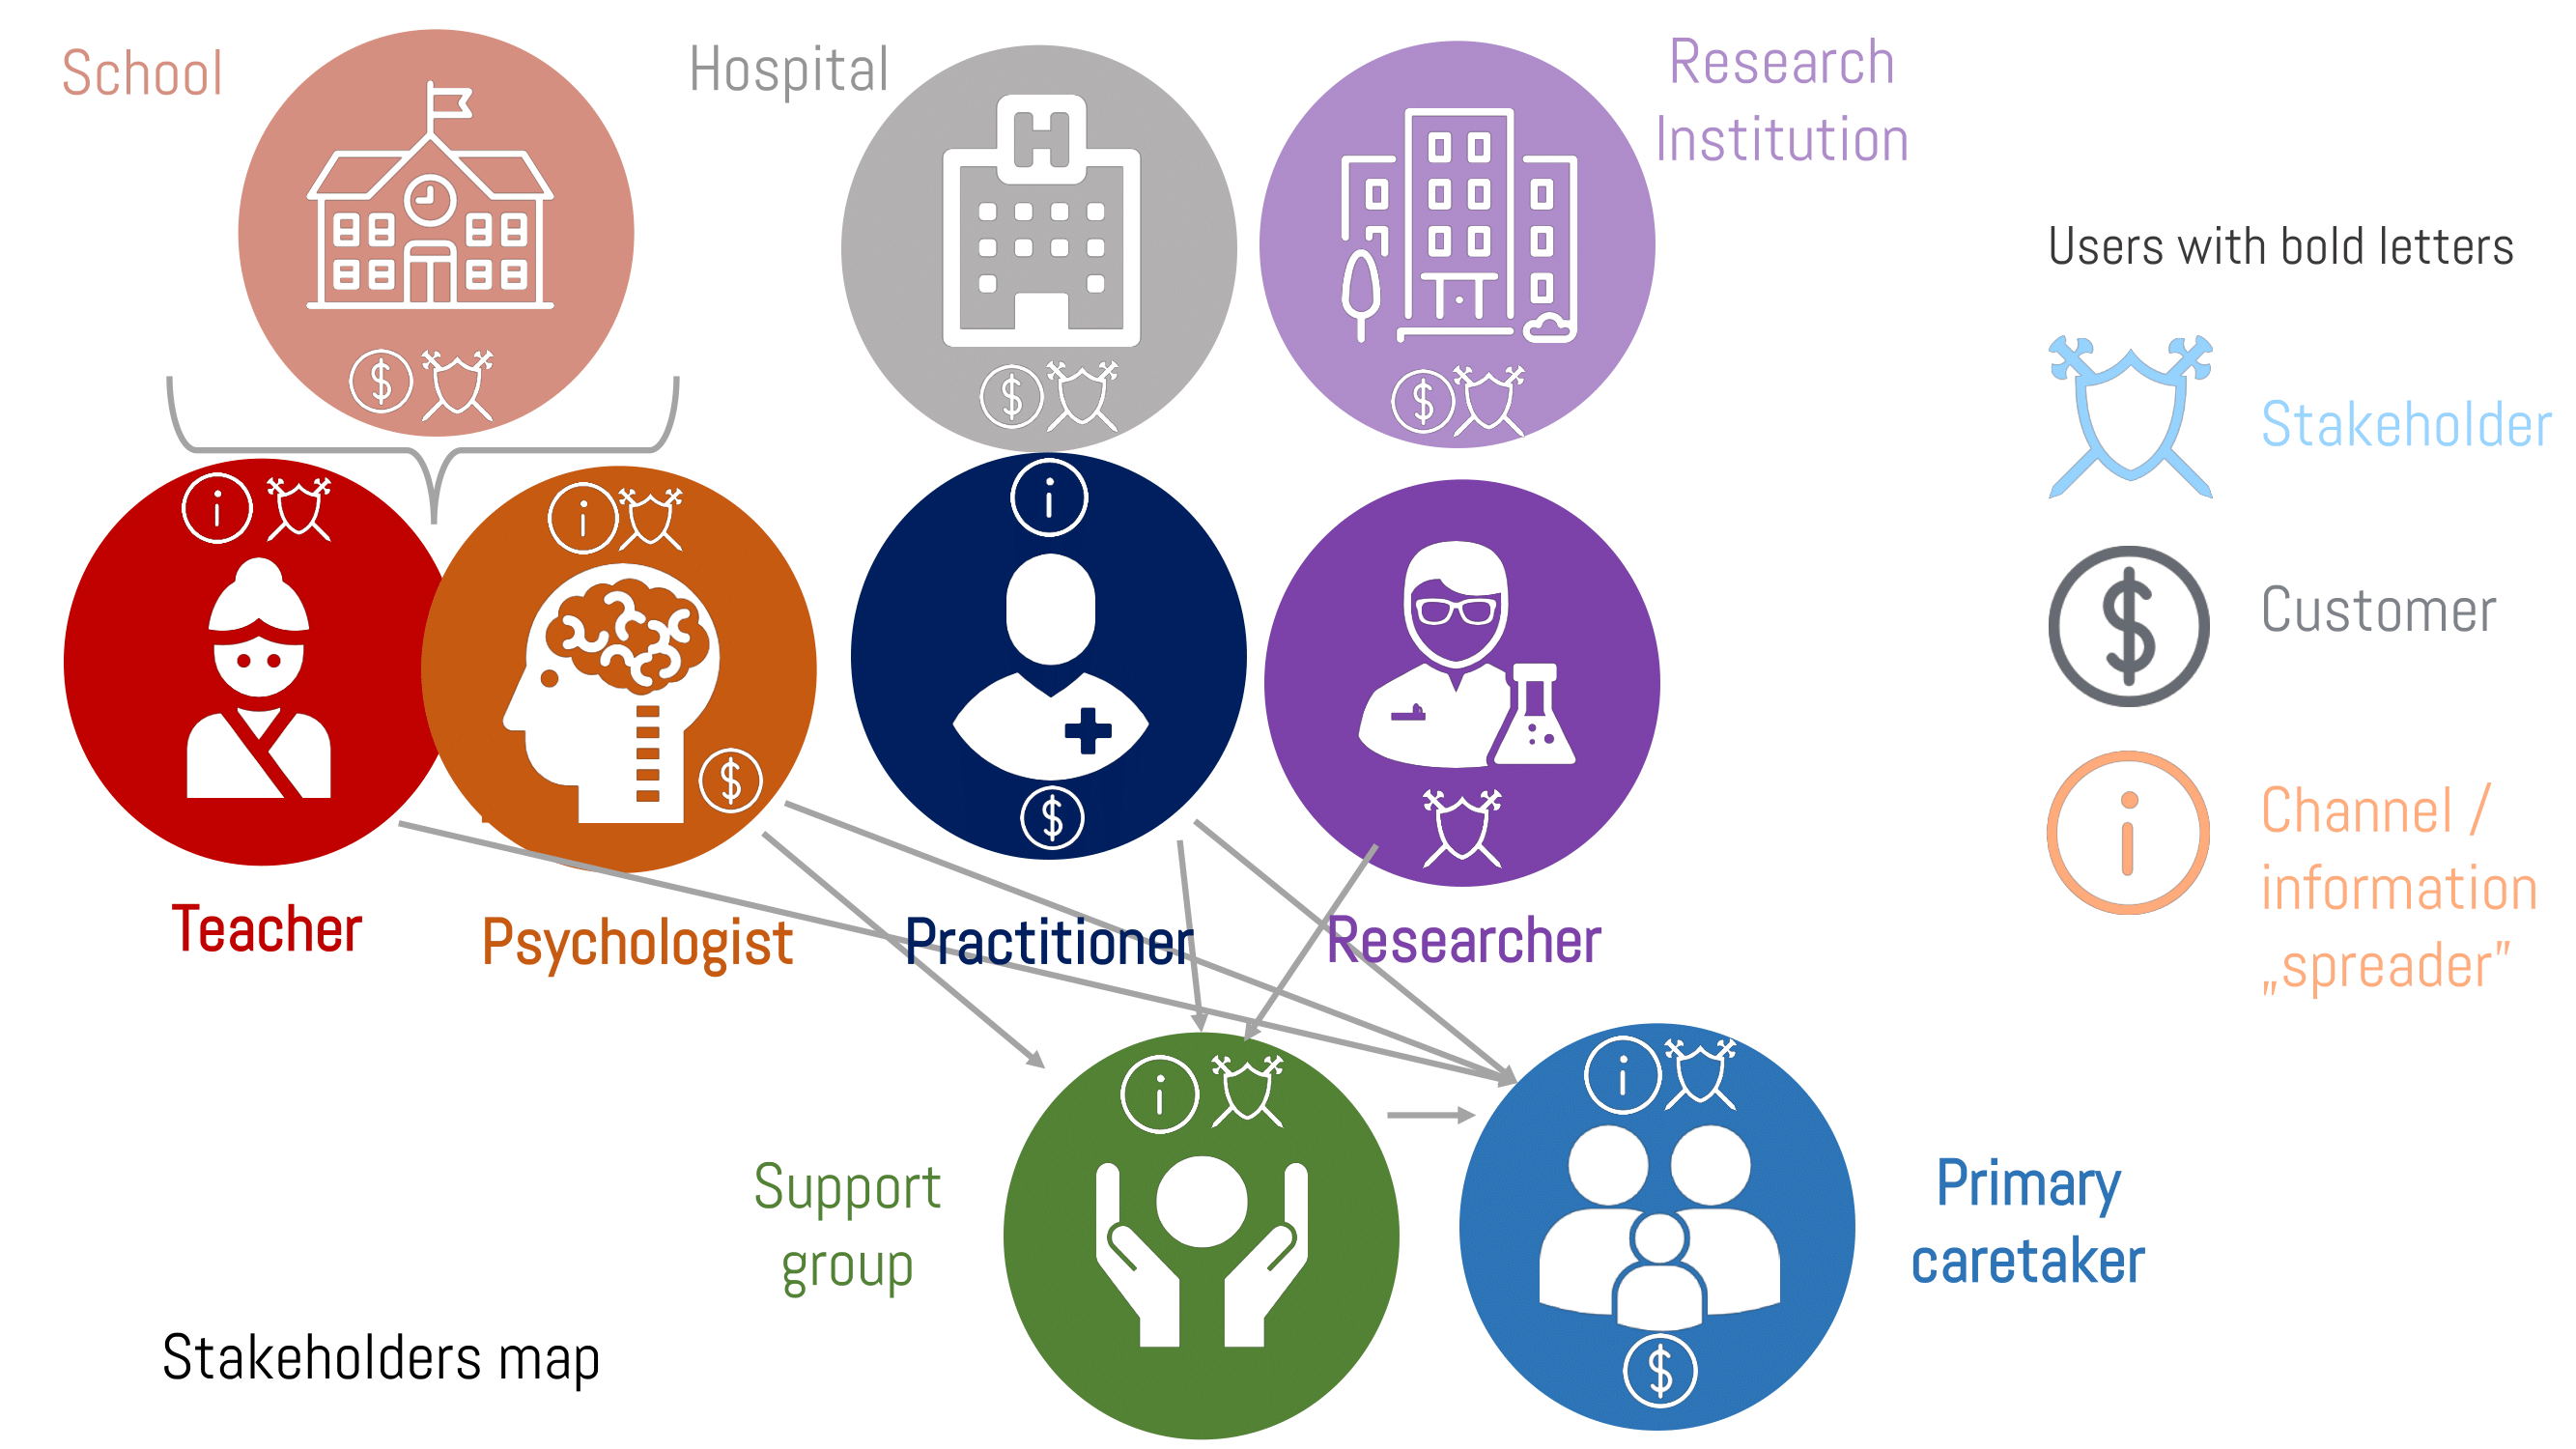
\includegraphics[scale=0.15]{stakeholder.png}
\caption{Main stakeholders involved the ADHD rehabilitation process}
\label{fig:stakeholders}
\end{figure}
 

\subsection{Special education for students with learning disabilities}

The spectrum of children having issues with learning or sustaining attention can be expanded to many other disorders beside ADHD. Rett syndrome, Autism spectrum disorder, and Dawn syndrome are also manifestations in which the child needs special help for proceeding with education. The market possibilities for ADHD were discussed in the previous section. In the following section, the market possibilities of special education institutions will be presented, working not only with children diagnosed with ADHD, but also with many other developmental disorders. 

\subsubsection{Statistics about students in special education}

The number of students ages 6-21 with disabilities rose to 5.83 million in 2014 , the most recent year for which statistics are available. According to the United States Special Education Enrollment statistics, the number of students having Autism spectrum disorder , once considered a low incidence, rose 165\% between the 2005-06 and 2014-15 school years nationwide.
Moreover, students with other health impairments including ADHD, epilepsy or mobility impairments, or mental-health issues such as bipolar disorder increased by about 51\% over that same ten year span. Figure \ref{img:special_st} and Figure \ref{img:special_kind} represent the trends of special education enrollment in from 1995-2014, demonstrating the increase and decrease of the prevalence of students with different disorders, based on the statistics of the U.S. Department of Education. \cite{samuels_2017}


\begin{figure}[hbt!]
\centering
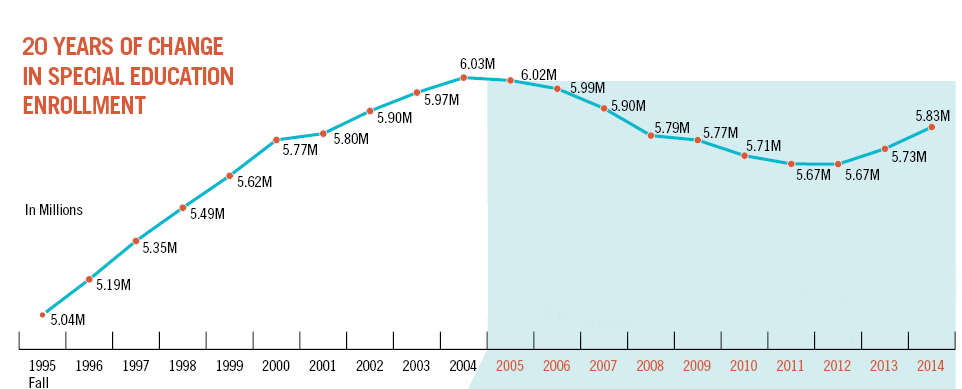
\includegraphics[scale=0.5]{specialeduenroll.png}
\caption[20 years of change in the special education enrollment]{20 years of change in the special education enrollment \textit{Department of Education Office of Special Education Programs IDEA Static Tables}}
\label{img:special_st}
\end{figure}
 
\begin{figure}[hbt!]
\centering
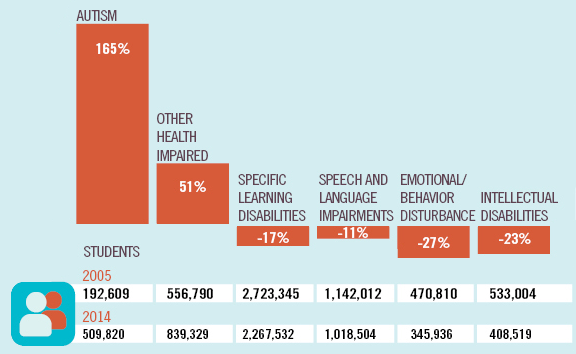
\includegraphics[scale=0.5]{kinds.png}
\caption[Percent if change in the number of students with specific disabilities]{Percent if change in the number of students with specific disabilities ages 6-21 between 2005-2014, \textit{U.S. Department of Education} }
\label{img:special_kind}
\end{figure}


\subsubsection{Special education providing schools}

A public charter school is a publicly funded school that is typically governed by a group or organization under a contract with the state. Between 2004 and 2014, the overall public charter school enrollment increased to 2.7 million . Based on the Individuals with Disabilities Education Act (IDEA), charter schools are required to provide special education for students with learning disabilities. In Figure \ref{img:special_schooltype}, the trend of public school enrollment is shown. By 2014, almost 3 million students attended charter schools. In Figure \ref{img:special_state} the percentage of public and charter school enrollment by state is illustrated.  After the District of Columbia (43\%), Arizona (19\%) and Colorado (11\%) had the next highest percentage of public school students enrolled in charter schools. In contrast, five states had less than 1\% of its public school students enrolled in public charter schools: Iowa, Kansas, Maine, Virginia, and Wyoming. \cite{spec_enroll}

\begin{figure}[hbt!]
\centering
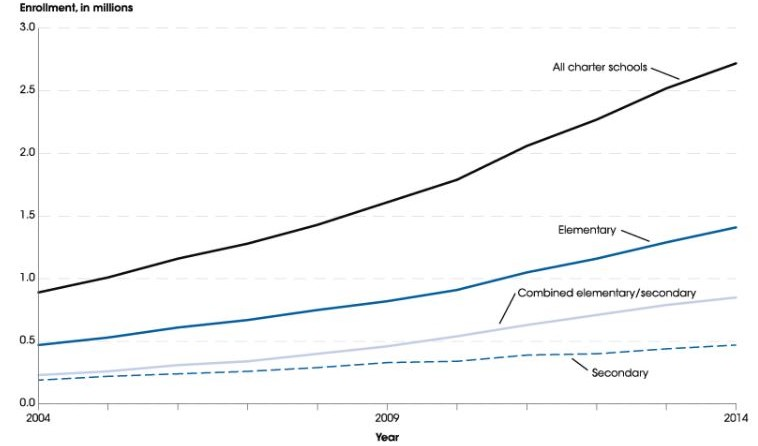
\includegraphics[scale=0.5]{charter.JPG}
\caption[Public charter school enrollment by school level]{Public charter school enrollment by school level, \textit{U.S. Department of Education, National Center for Education Statistics, Common Core of Data (CCD)}}
\label{img:special_schooltype}
\end{figure}
 
 
\begin{figure}[hbt!]
\centering
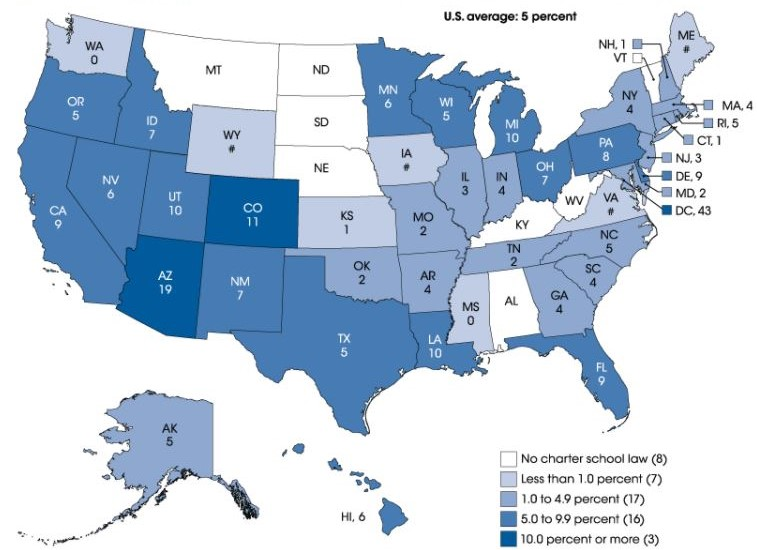
\includegraphics[scale=0.5]{percentagebystate.JPG}
\caption[Percentage of all public school students enrolled in public charter schools by state, 2014]{Percentage of all public school students enrolled in public charter schools by state, 2014, \textit{U.S. Department of Education, National Center for Education Statistics, Common Core of Data (CCD)}}
\label{img:special_state}
\end{figure}

In the special education field, there is a greater pressure on developing individualized education programs to ensure that goals are aligned to the standards and assessments that are being developed. Technology will continue to transform special education classroom instruction by increasing individual learning possibilities and enabling greater flexibility and personalization through the implementation of the use of electronics and web-based evidence-based practices. There is a big opportunity for Mindtech to enter this field, due to the openness of the market toward technology solutions.  \cite{scientific_learning_2017}


\paragraph{Market size}

As mentioned earlier, the IDEA agreement requires schools to provide special education for children with disabilities . Therefore, every school in the United States works with children with Autism spectrum disorder, ADHD, and other disabilities. 

\subparagraph{Total available market}

The total number of schools in the United States, including elementary and secondary schools, is 131,890, estimated by the National Center for Education Statistics. Not every institution focuses special attention on these students, so the number of targeted institutions must be reduced.

\subparagraph{Served available market}

In private schools, teachers have a lot more time to focus on the needs and personal development of students with special needs. Based on the estimation from the National Center for Education Statistics, there are 46,848 private and special elementary and secondary schools in the United States. However, these schools not only work with students with disabilities, so the focus is still divided among other students as well.

\subparagraph{Target market}

Mindtech's target market on the field of special education is special schools, specifically only students with disabilities. There are around 13,300 schools in the United States dedicated to working with students who have special needs , including private and public charter schools with approximately 6,482 and 6,747 institutions, respectively. These institutions have specialized curriculum and an experienced staff to overcome the challenges with special education. Their goal is to find the best practices and tools to provide a high-quality learning experience. Technologies that can empower students or teachers to reach a better learning experience are always interesting for this market segment.

\begin{figure}[hbt!]
\centering
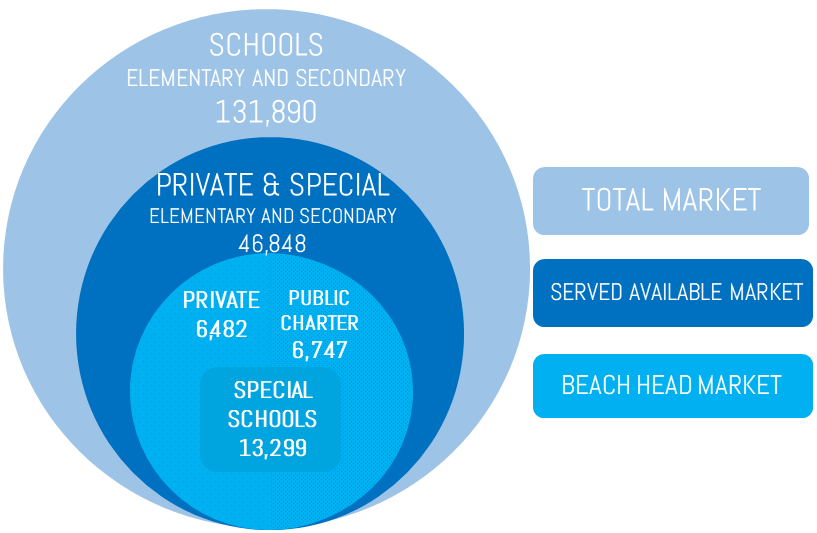
\includegraphics[scale=0.5]{charts.png}
\caption{Market estimation of special education providing schools}
\label{img:market_dropdown}
\end{figure}


\subsection{Locked-In Syndrome}
\subsubsection{Diagnosis}

Locked-In Syndrome (LIS) is a very rare condition caused by an infarct or trauma, leading to a damage in the ventral pons. The characteristics of the syndrome manifests in complete paralysis, but with the preservation of consciousness and cognitive skills. Patients retain vertical eye movement and blinking, facilitating non-verbal communication by eye movements. Besides these harsh conditions, ten years of survival rates have been reported in  80\% of the cases. \cite{smith_delargy_2005}. Although locked-in syndrome can affect anyone at any age,  most often the presentation is in adults, due to their higher risk for brain strokes and bleeding problems. \cite{phd}

LIS can be classified into 3 categories:  \cite{orphanet_LIS}
\begin{itemize}
\item \textbf{Classic condition}: preserved consciousness and upper eyelid and vertical eye movements
\item \textbf{Incomplete form}: patients still have limited voluntary movements other than vertical eye movements, most frequently of fingers, toes and head
\item \textbf{Total form}:  patients show complete immobility including eye movements but have preserved consciousness
\end{itemize} 

The diagnosis of LIS is a real challenge due to the patient's coma-like condition, and can be missed out if voluntary vertical eye movement is not detected from the unresponsive patient. Most likely a member of the care staff or family reports awareness when the patient is emerging from coma. Unfortunately there is no established treatment for locked-in syndrome, whilst supportive therapy for breathing and feeding is very important, especially at early stages. \cite{locked_webpage} In an ideal case, eye-based communication is established early with the patient, and if the patient is lucky enough to access it, brain-computer interfaces also aim to enhance the success of communication with several solutions.

\subsubsection{Statistics about locked-in syndrome}

LIS is classified as an orphan disease; its prevalence is currently unknown, but it is less than $1 / 10^{6}$. Based on the Orphanet's database, 33 cases had been published by 2009.\cite{orphanet_LIS}

To imagine what is like to be completely paralyzed without a voice, I would like to share some statistics from a study in 2007 involving 67 LIS patients. "44 \% of the patients suffered from chronic pain, 55 \% had anxiety and/or mood disorders, and 27 \% had suicidal thoughts. 67 \% envisaged resuscitation if needed, and two patients reported a wish for euthanasia." \cite{rousseau} Figure \ref{fig:lockedlife} summarizes the results of the study.


\begin{figure}[h]
\centering
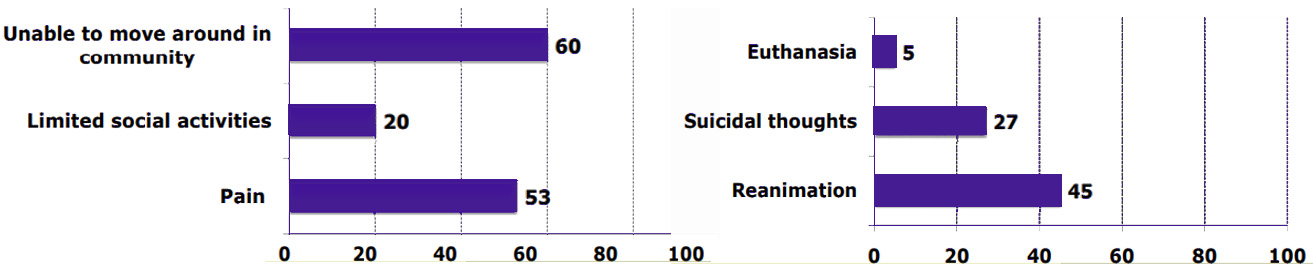
\includegraphics[scale=0.3]{lifeq.jpg}
\caption[Life condition of locked-in syndrome patients, self reported with a questionnaire]{ Life condition of locked-in syndrome patients, self reported with a questionnaire \textit{ALIS Questionnaire 2007} \cite{rousseau}}
\label{fig:lockedlife}
\end{figure}

\subsubsection{Current resources for locked-in syndrome rehabilitation}

\paragraph{Neuromuscular stimulation}

Rehabilitation programs are available for LIS patients, such as functional neuromuscular stimulation, which is uses muscle reflex stimulating electrodes to monitor the recovery of thumb, finger, head, and neck movements. This process is extremely important, since even the smallest movement can enable the patient to use a buzzer, an environmental control, or a communication device. Other treatments are symptomatic and supportive, seeking to improve the life quality of the patient. \cite{brainfacts} Since the majority of patients with LIS do not recover, most of the help for the patient focuses on life quality improvement. All patients with locked-in syndrome should be rehabilitated in a national or regional specialist center that has the specific multidisciplinary rehabilitation experience  and the proper condition. \cite{smith_delargy_2005} 

\paragraph{Communication with the patient}

There is a chance that LIS patients can learn to communicate by eye movements, although patients tire quickly through this process.\cite{smith_delargy_2005} In order to properly communicate with the LIS patient effective questioning skills must be used. Moreover it is essential to get the patient motivated: making the LIS patient able to receive commands (verbally, visually or written) and empowering to emit information in some way (yes/no blinking, alphabet tables, BCI devices). \cite{locked_laureys} Communication devices, such as patient-computer interfaces (infrared eye movement sensors, computer voice prosthetics) have a huge impact on the LIS patients liberty, empowering them to have real dialogues beyond the passive responding to any request of their caretakers. \cite{rousseau} 


\paragraph{Life quality of the patients}
\begin{tightcenter}
\textit{“Whereupon a strange euphoria came over me. Not only was I exiled, paralyzed, mute, half deaf, deprived of all pleasures, and reduced to the existence of a jellyfish, but I was also horrible to behold.”}
\newline
\textit{― Jean-Dominique Bauby (The Diving Bell and the Butterfly)}
\end{tightcenter}

A study from \textit{University of Liège} examined 10 chronic LIS survivors after their brain insult. The researchers neuropsychologically tested the patients on their short- and long-term memory, attention, executive functioning, semantic processing and verbal intelligence. They came to the conclusion that in most cases the cognitive functions of the LIS patients are not affected by the disease. These results are displayed at Figure  \ref{fig:lis_cogn} in comparison with healthy individuals. \cite{cognitive_lockedin}

\begin{figure}[h]
\centering
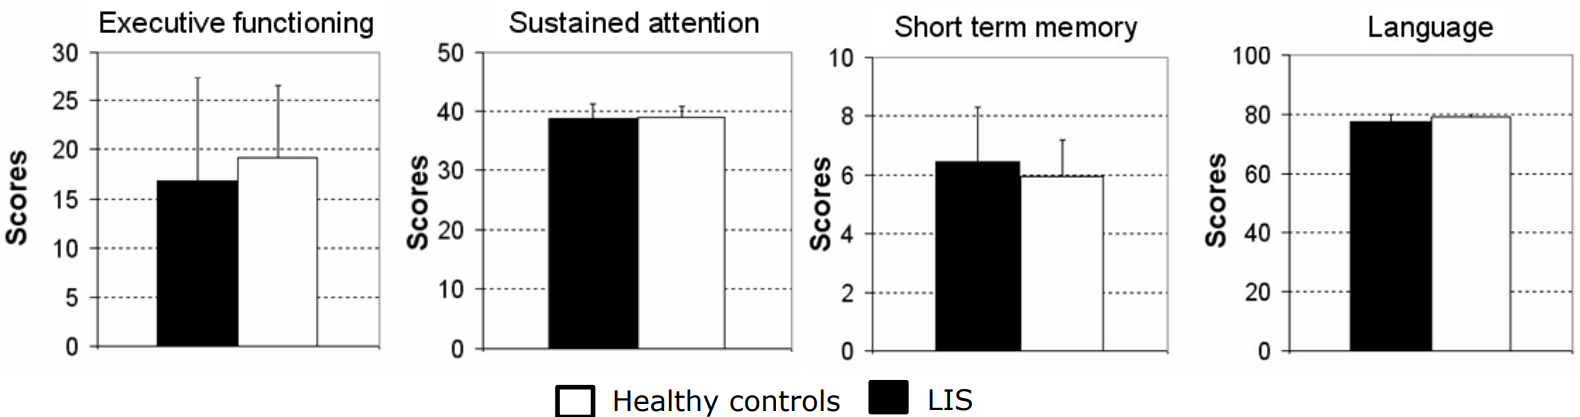
\includegraphics[scale=0.3]{lis_cogn.png}
\caption[Cognitive function in the locked-in syndrome]{Cognitive function in the locked-in syndrome \textit{University of Liège} \cite{cognitive_lockedin}}
\label{fig:lis_cogn}
\end{figure}


\subsubsection{Market analysis for locked-in syndrome solutions}
\paragraph{Market size}

\subparagraph{Total available market}
Dr. Niels Birbaumer from University of Tuebingen, who is one the leaders in the field of BCI, estimated the number of patients in need for a communication device in the US in the following way. There are around 500,000 ALS diagnosed patients in a year. After turning into vegetative state, some of the patients refuse treatment, some of them do not survive. Therefore only 5-6 \% of the patients want to live and communicate, which means approximately 25,000 patients need a brain computer interface a year. 35\% of these patients are locked-in syndrome patients, but unfortunately they are often misdiagnosed. So around 8,750 patients a year are in the state of locked in after ALS, but only 6,000 of them are correctly diagnosed.  \cite{niels} 

\subparagraph{Served market} This approximate number of 6,000 patients has to be reduced to the number of patients suffering from LIS classic or incomplete presentation, which would make approximately 4,000 patients a year. Patients with the total presentation of locked-in syndrome cannot be targeted with the Mindtech's technology yet as they are missing the ability of eye movements, and Mindtech's solution is based on blink detection.

\subparagraph{Target market} Our target market consists of LIS classic and incomplete diagnosed patients without any communication device, either being rehabilitated at home or at an institution. This number would be around 2,000 patients a year. Since Mindtech technology is really accessible. We are focusing on low-income families or rehabilitation institutions on a budget.

\paragraph{Market segmentation}

The market has two sides:
\begin{itemize}
\item B2C: the primary caretakers of the LIS patients
\item B2B: rehabilitation institutions, hospitals
\end{itemize}  

The LIS syndrome patients we can serve either have a classic condition  or an incomplete form, therefore we can target the caretakers of these patients. Special rehability institutions either in the private or public sectors are in our main focus, as well as hospitals with special sectors for LIS patients.


\subsection{Drowsy driving}

One of the biggest causes behind road accidents is the driver fatigue. When the drowsiness kicks in, especially while driving at a monotonous tempo for a long time, the driver loses concentration and the ability to react in time. This reckless phenomenon causes harm not only to the diver, but to the other passengers in the car, as well as the victims of the accident in case of a collision with another vehicle. In many cases, long and monotonous driving is inevitable, especially in certain professions (bus and truck drivers) and the drivers judgment on their own attention level is not trustworthy.
Several Original Equipment Manufacturers (OEMs) are looking to increase the implementation of driver monitoring systems in their vehicle model line-up, in order to reduce the number of accidents caused by drowsy driving. In addition, with that, Mindtech offers a solution which is not embedded in a specific passenger car, but accessible to everyone.
\cite{luxury}


\subsubsection{Statistics about drowsy driving and its consequences}

\paragraph{Accidents caused by drowsy drivers}

According to the National Sleep Foundation’s survey in 2006, 168 million admitted that they have driven a car while feeling drowsy in the past year, and 37\% of the drivers ($~$ 103 million) have fallen asleep at the wheel. 4\% ($~$ 11 million) of the subjects indicated that they have had an accident/near accident because they dozed off or were too tired to drive.

The National Highway Traffic Safety Administration estimates 100,000 police-reported crashes as a direct result of driver fatigue per year. 
This means 1,550 deaths, 71,000 injuries and \$12.5 billion in monetary losses. 
Since it is very difficult to attribute crashes to sleepiness, these numbers may be even higher in reality. 

\paragraph{Affected people}

Nearly 71\%  of adults in America drive a car to work according to NSF’s poll from 2011. Results showed that 27\% of these respondents admitted a tendency to drowsy driving to or from work at least a few days a month, 12 \% drove drowsy a few days a week, and 4 \% said they drove drowsy on a daily base. \cite{drowsy}

There are differences in drowsy driving tendency at different ages, gender and job type of the driver, which is summarized in Figure \ref{fig:dowsychat}.

\begin{figure}[h]
\centering
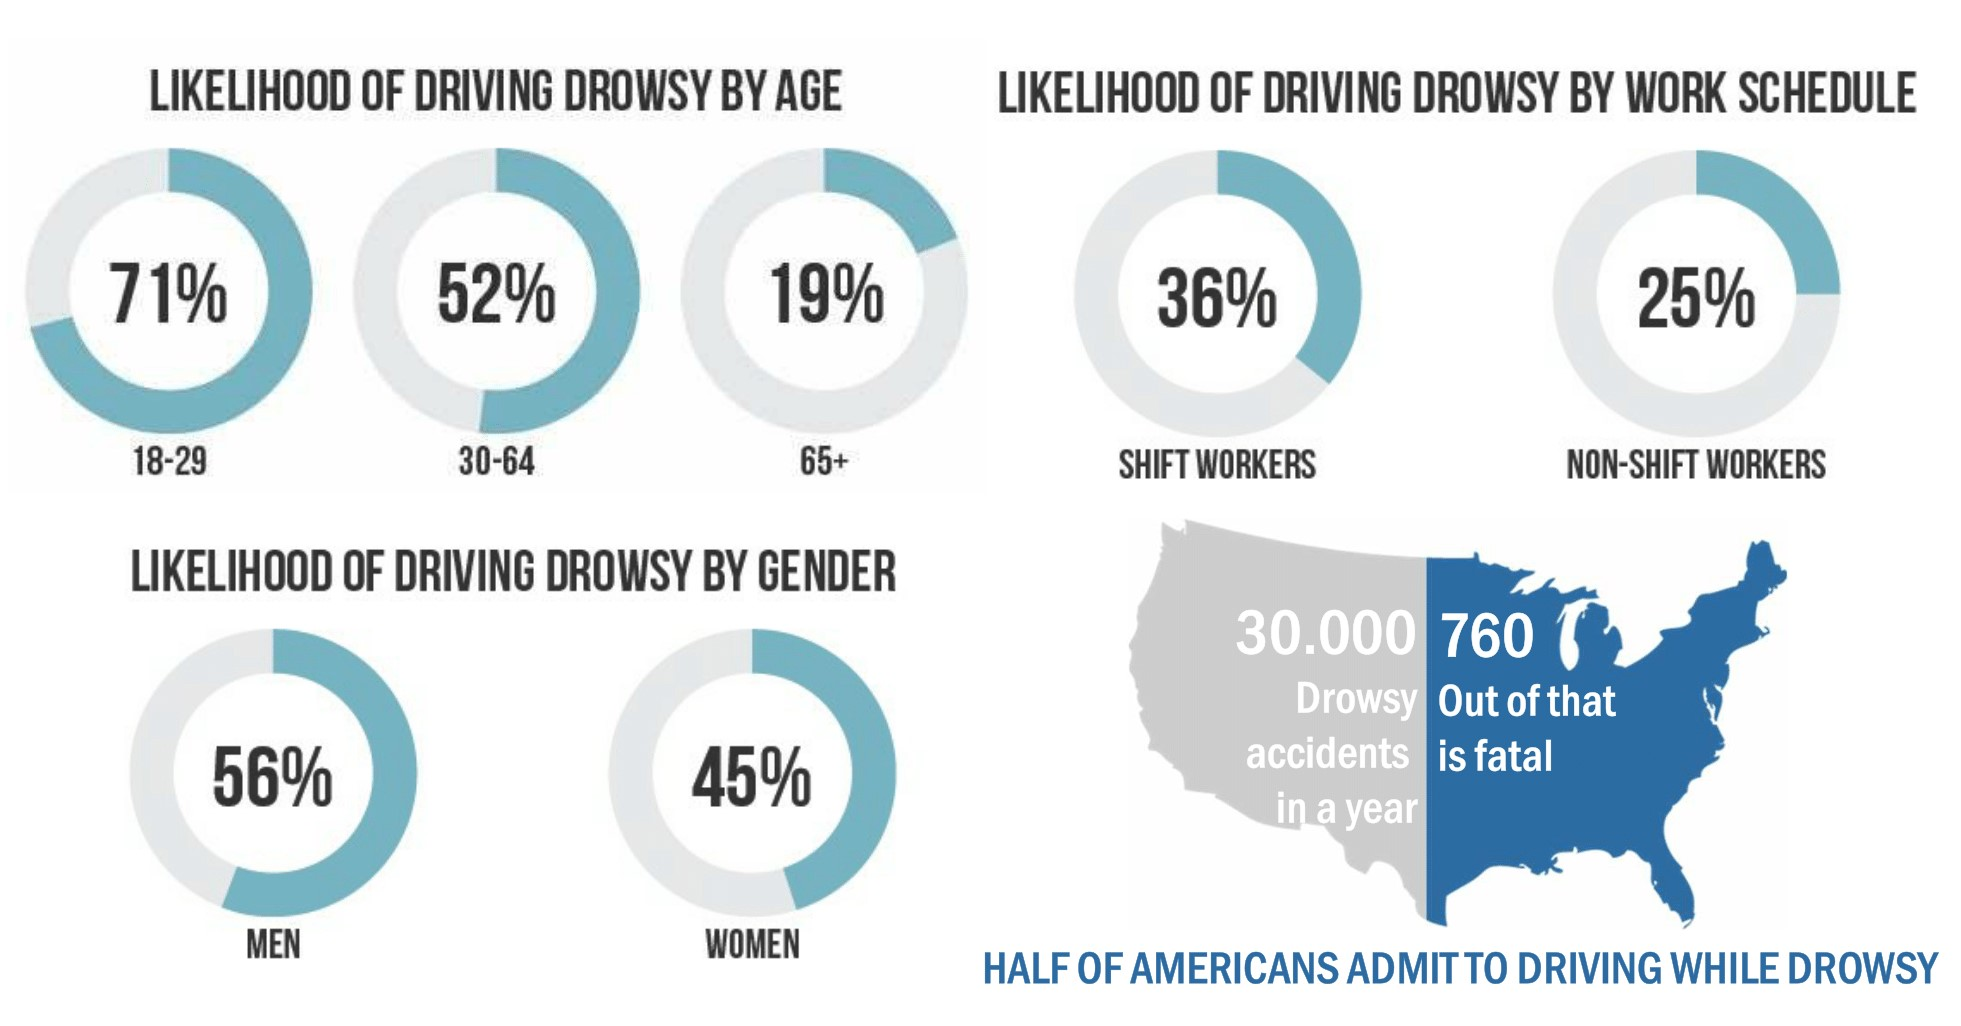
\includegraphics[scale=0.25]{drowsy_stat.jpg}
\caption[Statistics about drowsy driving]{Statistics about drowsy driving, according to the \textit{National Sleep Foundation} \cite{national_sleep}}
\label{fig:dowsychat}
\end{figure}

\paragraph{Cost of drowsy driving accidents}

Several drowsy driving incidents end with a jail sentence for the driver who caused the accident. The "price" for causing an accident is around multi-million dollars, awarded to families of crash victims. \cite{drowsy}
Generally speaking, the cost of automobile accidents related to sleepiness is between \$29.2 - \$37.9 billion dollars a year. Even these extremely high figures can underestimate the true number of accidents/near-miss accidents caused by drowsy driving, because  drivers are unaware or do admit that they were drowsy at the time of the accident. \cite{drowsy_sleepfoundation}

\subsubsection{Driver attention monitoring possibilities}

Original Equipment Manufacturers are showing interest in offering holistic Driver Monitoring Systems (DMS) by equipping cars with technology that provides information about the state of the driver, including fatigue, cognitive load,  and health monitoring \cite{f&s_car}

Driver attention monitoring systems are analyze driver behavior, and detect the biological patterns occurring micro-sleep situations. They issue appropriate warnings to alert the driver and revive their attention. The system can help bring the attention of the driver back onto the road and reduce sleep-related crashes.  \cite{f&s_car}

There are several approaches to create a DMS, with different technological solutions involved. The alertness level of the driver can be determined from actions such as speed, lane discipline and eye movements (outside components), or from the root of the driver's actions the biomedical signals from their body; for example heart rate, brain waves and respiration (inside components).

To monitor the outside components, vision based solutions are accessible: 3D cameras, face recognition softwares focusing on gaze concentration and direction. For the real time detection of biological signals related to attention levels, wearable sensors are available such as pressure transducers, smart devices and epic sensors (ECG, EMG, EOG and EEG measurement). The overview of the possible technologies in driver monitoring are presented in Figure \ref{fig:techdms}. %% mmore explnation on the Figure

\begin{figure}[h]
\centering
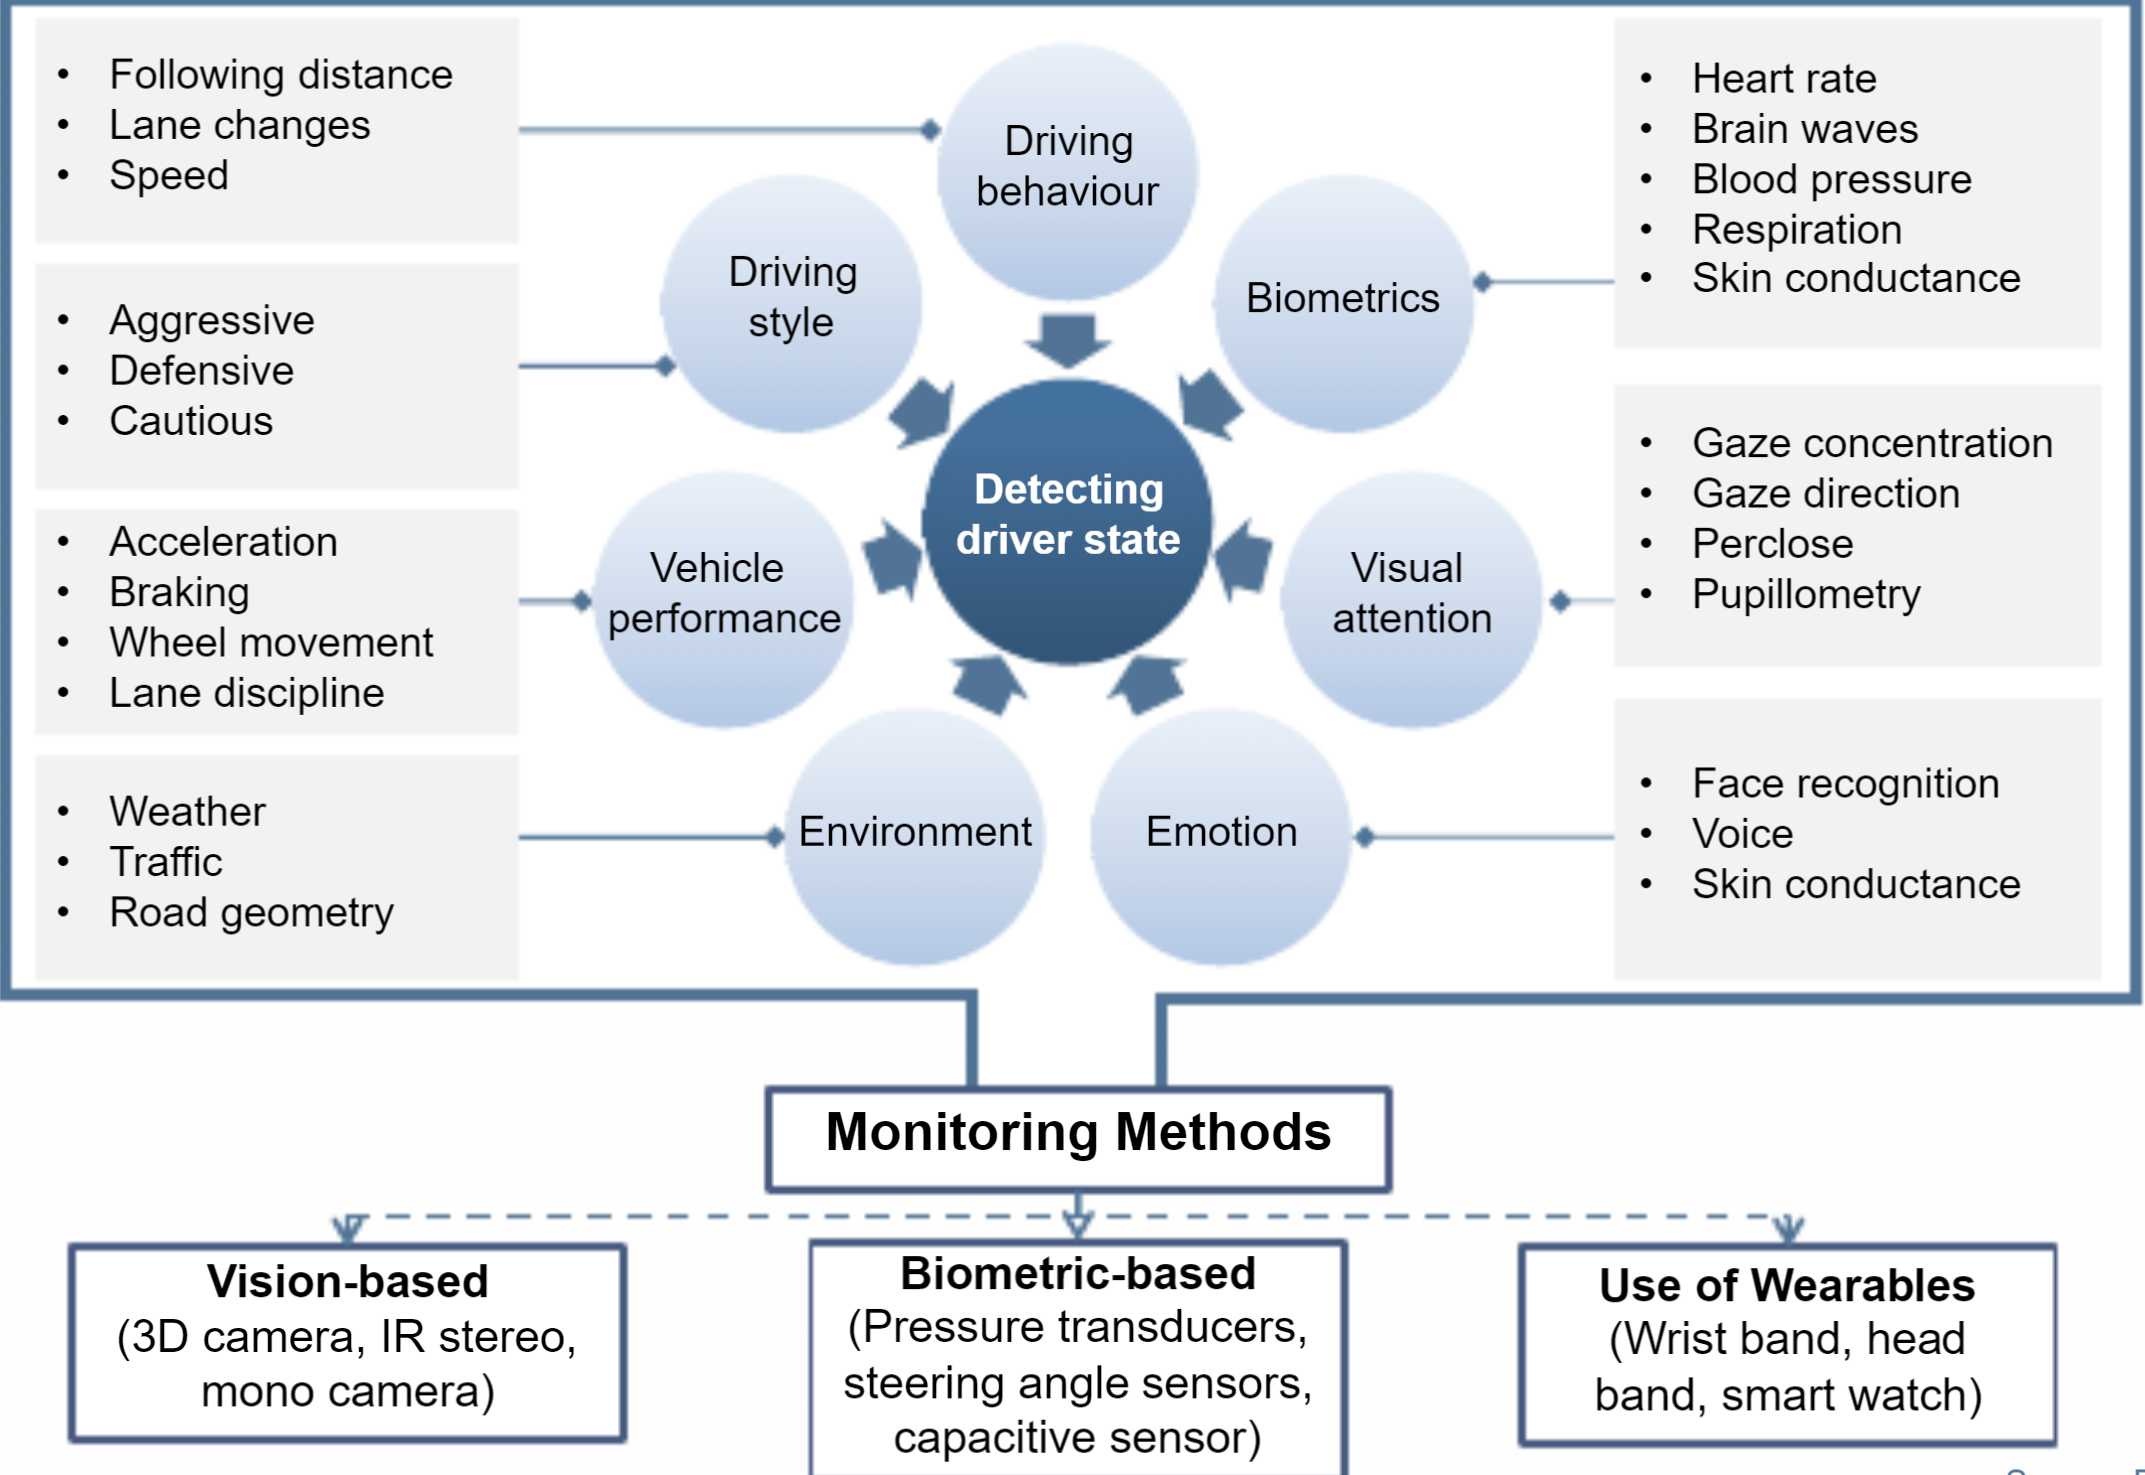
\includegraphics[scale=0.4]{DSMsonsors.PNG}
\caption[Possible monitoring parameters in DMS]{Possible monitoring parameters in DMS\cite{f&s_car}}
\label{fig:techdms}
\end{figure}


\subsubsection{Market analysis for driver attention monitoring}

\paragraph{Market size}

\subparagraph{Total available market} 60\% of adult drivers (168 million) admitted driving drowsy based on the previously presented statistics. But not only driver who admit to driving drowsy are affected, therefore the total market is the around 200 million drivers, who are in danger of drowsy driving. \cite{drowsy} 

\subparagraph{Served market} The served market can be found by subtracting the number of people who own a car with some kind of monitoring system, who not drive for long hours frequently, or not being familiar with the usage of smart device technology on the road. In total, our served market is around 100 million drivers, including professionals (truck and bus drivers) and people forced to drive long hours to work or for personal travel purposes.

\subparagraph{Target market} Our target market is long term professional drivers and the company hiring them and daily or weekly long term drivers with a higher need for security. There are 3.5 million professional truck drivers in the United States estimated by the American Trucking Association \cite{trucking},  169,680 bus drivers from which 20,500 are part of Interurban and Rural Bus Transportation, and 3,340 drivers working within Scenic and Sightseeing Transportation \cite{bus}. 

\subparagraph{Market segmentation}
We have a 2 sided market:
\begin{itemize}
\item B2C: long hour drivers daily on weekly basis 
\item B2B: transportation companies, trucking companies
\end{itemize}  

B2C for long hour drivers daily on weekly basis, living a lifestyle with a big attention to their health and safety. The B2B side is represented by the transportation companies, with a need to keep their customers safe by monitoring their bus drivers. Besides that we will target companies on charge of truck drivers.

\subsection{The ideal solution} 

All three cases presented above have one thing in common: the lack of a portable, affordable and innovative technology which could help with cognitive skill development, can create a bridge of communication or even prevent driver fatigueness which leads to accidents. By measuring frontal lobe activity, where we can easily filter out the brainwaves standing for attention and blinking signals, we can solve all the above mentioned problems with one technology.

\subsection{Drawbacks of existing solutions}

ADHD treatments are either managing only the symptoms (medication) or are inaccessible for most of the affected patients. Most schools lack a well trained school psychologist, professional therapist are not available in every location, and insurance does not cover the special therapy fees in most cases. In addition the teacher and psychologist communication is not always well developed.

The locked-in syndrome communication devices are either in the research and development phase, or are enormously expensive for the affected families. These devices are usually large in size with a complexity requiring special assistance to use.   

The current driver alertness monitoring systems are not well established yet, however there are attempts from several car manufacturing companies to introduce solutions, aiming to provide a bio sensory system for this purpose. Although the utilization of brain data is expected to be introduced in the distant future,  the current solutions are only available for the specific model owner, but not the public.

\subsection{Mindtech's solutions}

\subsubsection{Mindtech's solution for ADHD}

Current Neurofeedback trainings are not only expensive, but stressful for the patients and primary caretakers, while they consume a lot of time and are carried out in laboratories and hospitals.

Mindtech is helping with the therapy of children having attention problems by monitoring real time attention level (based on EEG data) with an accessible solution, combining a portable EEG measuring headset with a smart device application. This solution empowers  educators and psychologists to decide whether the child  is concentrating on a certain task or not. With the help of this application, the teachers will be able to choose the right development methods and tasks for every child. Even the  patient diagnosed with ADHD is able to take care of their own therapy by using the NeuroSky headset ant the Mindtech  android/iOS based application on a smart device.

Mindtech helps find the best rehabilitational practice for everyone by providing a system that can continuously give feedback about attention, in parallel with using any cognitive improvement software or perform a specific task. The system consists of a NeuroSky EEG headset and a smartphone with the TrainDHD application.  While special education trainers are performing various training tasks, our software processes the patients brainwaves and finds the task that caused the highest raise in attention level. Therefore the system helps special education teachers to “take a look” at the patients brain.
During the automated neurofeedback training patients are watch their favorite movies. If they are paying attention, the movie is clearly visible. As soon as the patient is not paying attention, the video starts to fade into black. With the help of our system, trainings can be carried out in any environment lowering the stress factor affecting patients. 


\subsubsection{Mindtech's solution for locked-in syndrome rehabilitation}

In order to increase the standard of living for persons paralyzed, Mindtech is developing therapeutic mobile applications in Android and iOS, enabling interactive communication. The reader-, writer- and memory game applications are controlled by blinking signals, recorded by a NeuroSky EEG headset. 
The application can be personalized to the users profile, based on the patients capability of blinking. 

\subsubsection{Mindtech's solution for driving alertness}

The drive alert application is unique its own way: none of the waking systems built in specific cars can detect attention problems. These features are build only for keeping divers awake. This Mindtech application creates a value by saving lives on roads: truck drivers, bus drivers and every person traveling can be kept secure with this system.
Mindtech uses real time brain data with the use of a NeuroSky headset, and warms the driver before an accident occurs. In this case tthe driver is not qualified for continuing the driving without taking a break.


\subsection{Choice of market}

Mindtech can serve the three different areas of innovation, with a very strong and easily adjustable brain wave processing technology. With the tool of the NeuroSky brainwave measuring headset, and a smart phone device, Mindtech can empower its users to improve cognitive skills, communicate with their environment, or prevent accidents. The Android/iOS platform used for rehabilitation is a fresh new market. Mindtech is developing Android/iOS applications, processing, and displaying the real time brain data with the best algorithms possible. 

Based on market analysis I found that the market of learning disorders is the primary market I would like to examine further; it is worth examining the market possibilities of the different subsegments. The ADHD only approach has many Besides that I am mapping the case of locked-in syndrome and drowsy driving cases as two strong secondary markets for the further validation.


\subsection{Goal of this thesis}

The goal of this thesis is to find the right market for Mindtech to enter with its technology after conducting  customer validation and minimum viable product testing. At the end of the thesis a complete launch strategy and business plan will be ready for Mindtech to enter the US market.
In order get better insight about the companies market strengths , I continue to present an overview about existing technologies, focusing on Mindtech's solutions. 



%%%%%%%%%%%%%%%%%%%%%%%%%%%%%%%%%%%%%% CH 2 %%%%%%%%%%%%%%%%%%%%%%%%%%%%%%%%%%%%%%%%%%


\newpage
\vspace{100mm}
\begin{center}
\uppercase{\Large{Chapter 2}}
\section{\uppercase{\large{BCI TECHNOLOGY AND ITS POSSIble applications on the therapeutic and attention monitoring markets}}} % change
\vspace{20mm}
\end{center}

%\setcounter{section}{2}
%\renewcommand*{\thesection}{\the\value{section}}

\subsection{Introduction}


As presented in chapter one,  two neurological disorders (ADHD and locked-in syndrome) and the issue of driver alertness hold big challenges and market potential. In the following chapter I will discuss the existing traditional and technological approaches  for the solution of these problems, furthermore I will introduce and examine in detail Mindtech's solution and technology, along with its competitive positioning on the market.

\subsection{Traditional approaches to the problems}


\subsubsection{Traditional solutions for ADHD disease}

After diagnosing ADHD the main questions left to address involve treatment—whether the child is sufficiently impaired to need medication (primary care question), therapy (mental health), or special services (education) and then to evaluate treatment outcomes. \cite{pelham_fabiano_massetti_2005}

One in five American children who have been diagnosed with ADHD are not receiving medicine or mental health counseling for their disorder. \cite{healthline_adhd}
About 1 in 10 children with special health care needs with ADHD were receiving neither medication treatment nor behavioral therapy. \cite{adhd_general}

There are several possibilities for behavioral management trainings, such as behavioral parent training (BPT), behavioral classroom management (BCM), and behavioral peer interventions (BPI) BPT and BCM meet criteria for well-established treatments for ADHD. \cite{pelham_fabiano_2008}

The effective behavioral management trainings are only possible with the strong contribution of psychologists (private therapist or school psychologists), parents, and teachers. There are traditional tools such as daily report cards, which share feedback on the child's behavior from the teacher to the parents, but this communication system is not digitized yet.

\subsubsection{Traditional solutions for Locked-in Syndrome}

Locked-in syndrome patients can learn how to communicate through eye movements, if the primary caretakers learn how to use  effective questioning and if the patient is motivated to engage in  conversation. The patients receive information either verbally, visually, or written, and then they answer with the method of yes/no blinking or an alphabet table. \cite{locked_laureys}

\subsubsection{Traditional solutions for driver alertness}

There is no direct solution for driving alertness monitoring or awakeness increasing with significant effectively rate without technology involved. Drivers can only use practices to extend  or force to extend, their alertness levels by drinking coffee or energy drinks. As an indirect solution, having a companion in the car or listening to the radio can help force the attention to a level acceptable for driving.


\subsubsection{Drawbacks of the solutions}


\paragraph{ADHD}The market of ADHD medications is constantly growing, the use of medications does not exclude the need for other methods. Medications are only targeting the symptoms and not the impairment. Impairment are solved by either behavioral or neurofeedback trainings. These trainings are not just rare to access, are expensive for the parents, but also they are not effective enough because of their low frequency.

\paragraph{Locked-in Syndrome}Communication with the patient with locked-in syndrome through yes/no blinking and alphabet tables is mutually tiring for the patient and the caretaker as well. Technology driven solutions are highly needed to increase both the quality and efficiency of communication. 

\paragraph{Driver alertness} None of the above mentioned techniques solve the problem of insufficient driver alertness levels after hours of monotonus driving. Energy drinks, companion or loud music can only force the driver to stay awake, but cannot create the needed cognitive state for attentive and careful driving. 


In summary it is clear that more advanced solutions and the innovative power of technology is needed to overcome the challenges of these problems. In the next section I would like to introduce the technology of Brain Computer Interfaces, which overcomes the barrier of decoding the human brain activity.

\subsection{Brain Computer Interfaces}

The possible usage of Brain Computer Interfaces is one the most examined and challenging areas in Healthcare and Consumer Electronics. The non-invasive BCI is already revolutionizing areas of medicine with motor restoration, wheelchair assistance, and treatment of several neurological disorders. The BCI market is  growing significantly due to its utility in a number of medical applications. \cite{bci_fs} Along with that the wearable device industry is undergoing an increase in trend during the last few years. The Health care market is expected to agilely increase for wearable devices with targeted application for medical scenarios. \cite{wearable}

\begin{figure}[h]
\centering
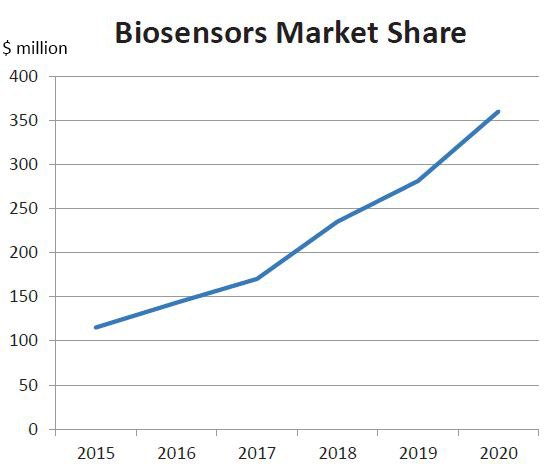
\includegraphics[scale=0.5]{biosenzors_market_2015_2020.png}
\caption[Biosensors Market forecast by 2020]{Biosensors Market forecast by 2020 \cite{wearable} The wearable biosensor market has 13 \% share of the wearable healthcare devices. The market is at \$115 million and it’s expected to reach \$360 million by 2020.}
\end{figure}
 
\subsubsection{BCI Technology}

A brain computer interface is an innovative technology, with the power to radically override the way that humans interact with the environment and with each other. By empowering the user to create a connection between their brains and the outside world, a BCI device makes it possible for people who can’t communicate to speak their minds. This technology even has the potential to became an extension of the human body. \cite{neurosky_bci}

A BCI is a device that consists of three important parts: a sensor that measure brain signals, an amplifier to enhance the faint brain signals, and a computer that decodes the brainwaves into a control signal for computer softwares and/or smart devices. The components of BCIs can be embedded in the human brain (invasive solution), or made portable and/or wearable (non invasive solution). 

BCIs are being developed for a variety of applications and types of users. Rehabilitation devices sim to help people recover from injuries and are intended to permanently replace a function that has been lost or impaired due to injury or disease. There are temporary BCIs for game controllers, based on technology that measures brain signals with electrodes built into a cap or headband. \cite{utrech_neuroprosthesis}

The BCI system consists of 4 building blocks: signal acquisition,  feature extraction, translation algorithm, and  device commands. \cite{bci_abra} An overview of this process can be examined in Figure \ref{fig:bci_abra}

\paragraph{Signal acquisition} Signal acquisition is the measurement of brain signals using a sensory unit. There are several neuroimaging methods available; I will focus on their characteristics in a different subsection. At this state, the signals are amplified to levels suitable for electronic processing and they also undergo filtering to remove electrical noise or other unwanted signal characteristics. Finally the analog brain signals are converted to digital signals. \cite{kapreans}

\paragraph{Feature extraction} Feature extraction analyses the digital signals in order to distinguish relevant signal characteristics. In order to later create a control signal for the computer, the features should have strong correlations with the user's intent. \cite{kapreans}

\paragraph{Translation algorithm} Translation algorithm converts the selected characteristics into suitable commands for the output device. For example, selecting a specific letter on the screen, appearing in a specific signal feature in the brainwaves, would be transformed to the selection command form.\cite{kapreans}

\paragraph{Device command} Device command is operates the external device, providing feedback to the user evoking the task.\cite{kapreans}

\begin{figure}[h]
\centering
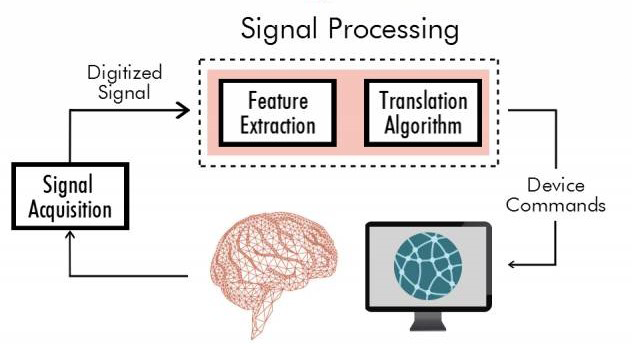
\includegraphics[scale=0.6]{bci_abra.png}
\caption[BCI system sequential components]{BCI system sequential components \cite{bci_abra}}
\label{fig:bci_abra}
\end{figure}

\subsubsection{BCI Market} 

The Brain Computer Interface has a wide range of possible applications, covering medical, industrial and military demands. The market of BCI can be categorized to 3 subgroups. 
From the product perspective, the interface can be either invasive, partially invasive or non-invasive. 
Invasive BCIs generally use electrodes that are implanted directly into the grey matter of the brain during neurosurgery. Partially invasive BCI use electrodes that are mainly implanted in the skull and exterior to the brain. Non invasive BCI scanning devices are mounted on caps or headbands placed on the user. \cite{kapreans} The non-invasive feature makes the product approachable and more desirable to use, minimizing discomfort to the user. 
From the application point of view, BCI devices are appearing in healthcare, entertainment (especially gaming), neuromarketing and neurofeedback industries. From the end user side, there is a large need for BCI technology in medical, military and indrustrial fields. \cite{bci_fs} Figure \ref{fig:bcimarketsegm} represents the possible cathegorization of the BCI market.

\begin{figure}[h]
\centering
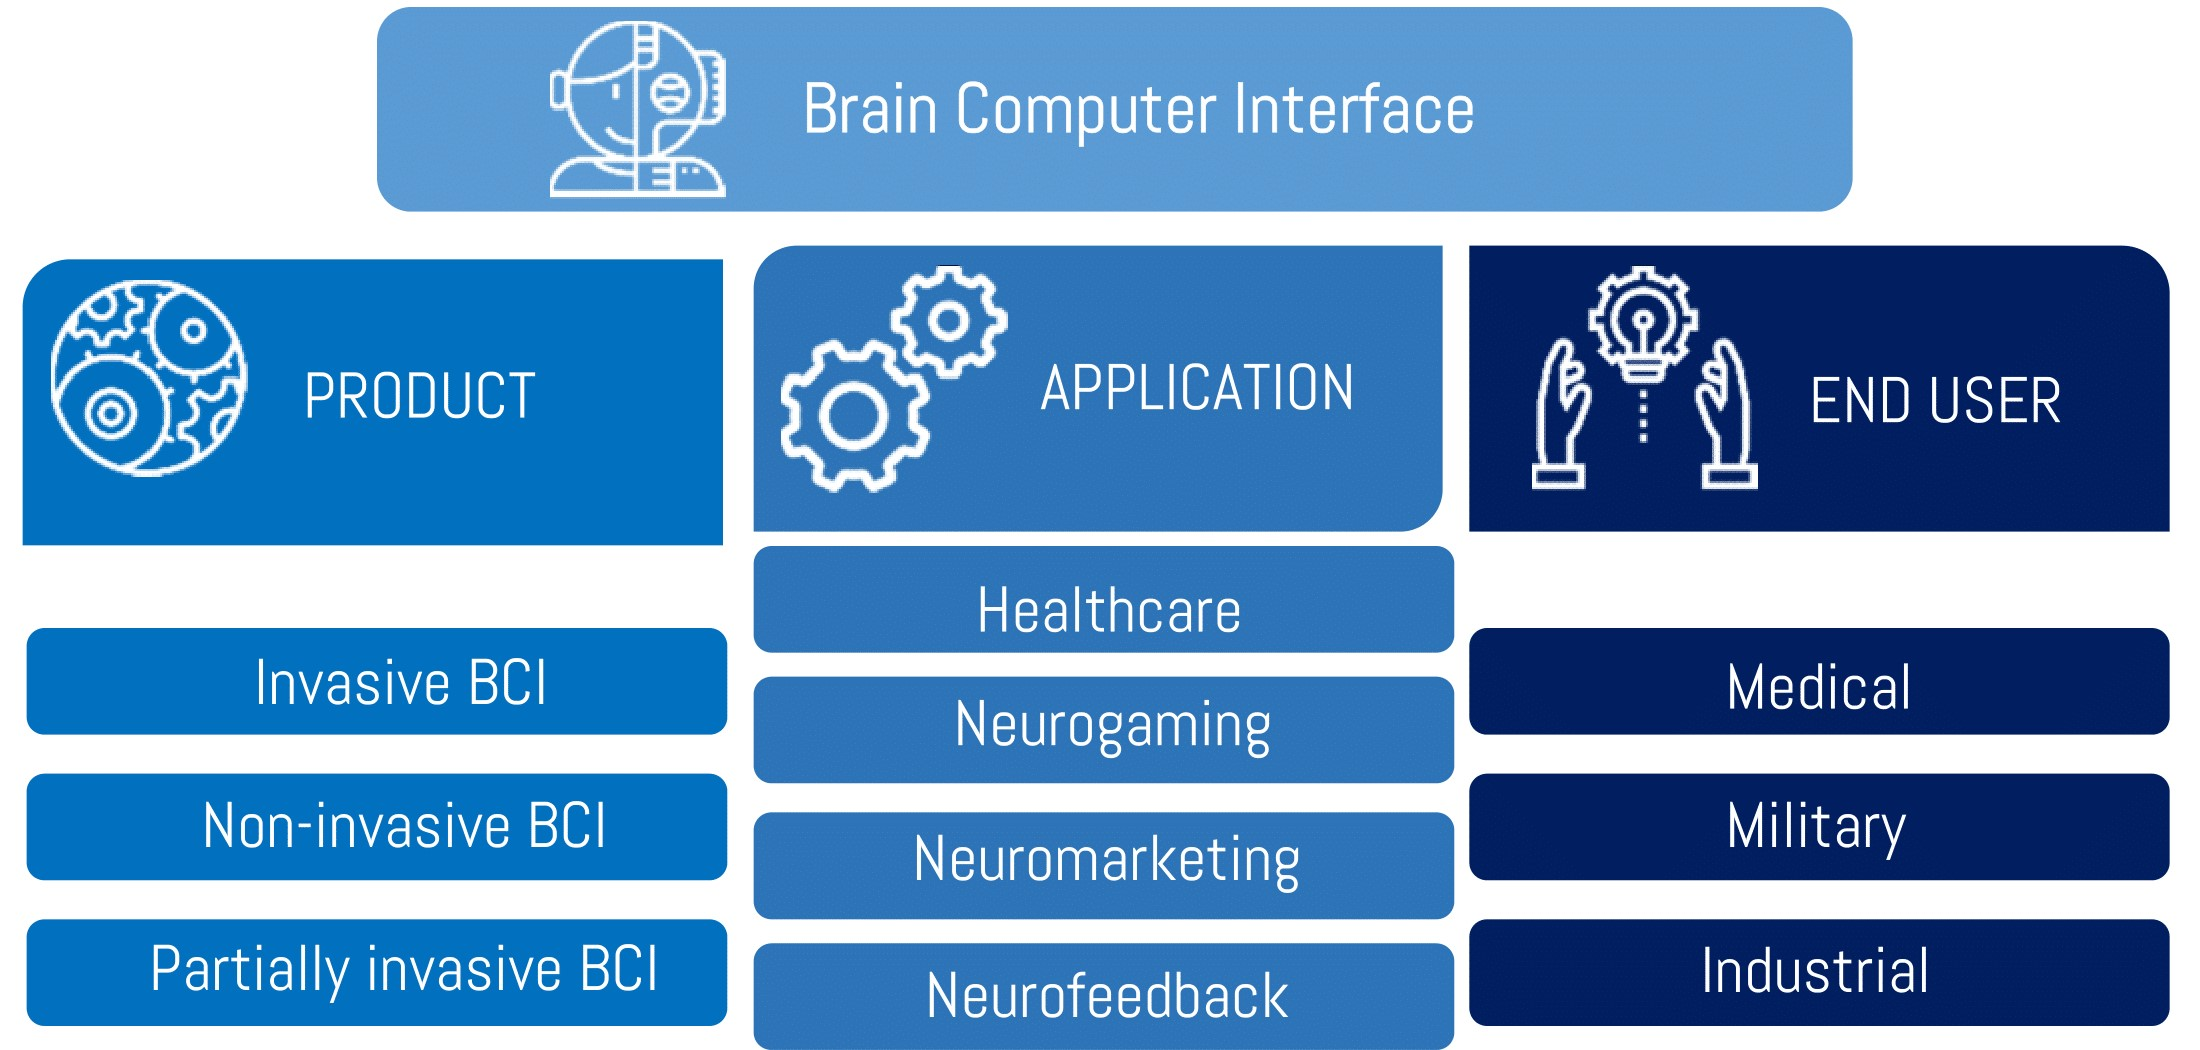
\includegraphics[scale=0.21]{bci.JPG}
\caption[Market segmentation of BCI Market]{Market segmentation of BCI Market \cite{bci_fs}}
\label{fig:bcimarketsegm}
\end{figure}

The  Brain Computer  Interfaces  market  is  majorly  a  fragmented  market,  with  greater part  of  key  stakeholders in  North America and Europe. Although, among all these manufacturers, most of participants are small and medium enterprises (SMEs) or early-stage startups. \cite{bci_fs} In Figure \ref{fig:bci_market} we can see that startups are already on the market both in the medical application (2.0 \%) and technology fields (20.0 \%).  
.
\begin{figure}[h]
\centering
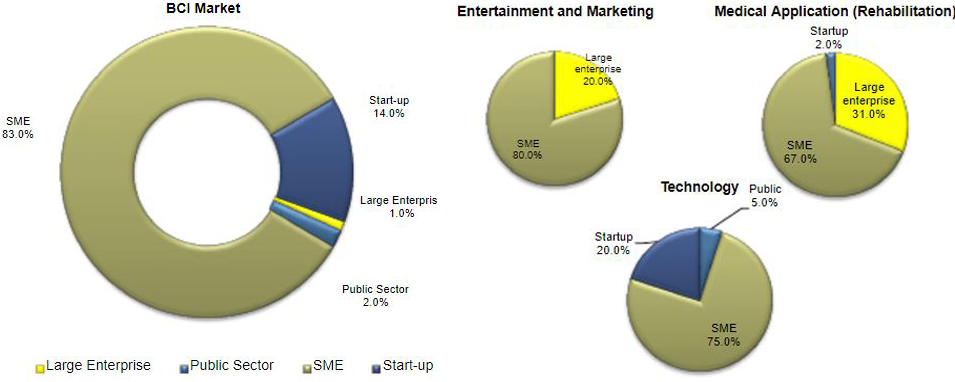
\includegraphics[scale=0.6]{marketBCI.png}
\caption[Market Segmentation of BCI Market and BCI-associated Industry Stakeholders Arranged by Sector]{Market Segmentation of BCI Market and BCI-associated Industry Stakeholders Arranged by Sector \textit{According to the European Commission within the 7th Framework Programme in 2015}} \cite{bci_fs}
\label{fig:bci_market} 
\end{figure}

\subsubsection{Neuroimaging methods}

There are several neuroimaging methods available, from the invasive type of interaction to the non invasive way of interaction with the user/patient. Although the development of sensory technology is still in a growing phase, with big challenges to overcome, there are already some good approaches to the brain activity measurement.

Comparing the existing sensory methods, we can conclude that the Electroencephalography with its high temporal resolution and low cost of initial setup is the most ideal for BCI applications. Although, it is prone to signal artifacts and in some cases cannot provide the necessary information by itself (signals are noisy and variable in nature), its features of non-invasive nature and portability empowers users from clinicians to everyday users to collect data easily. \cite{bci_fs} The comparisons of possible imaging methods are gathered in Table \ref{img:imaging_dev}. 

\begin{figure}[h]
\centering
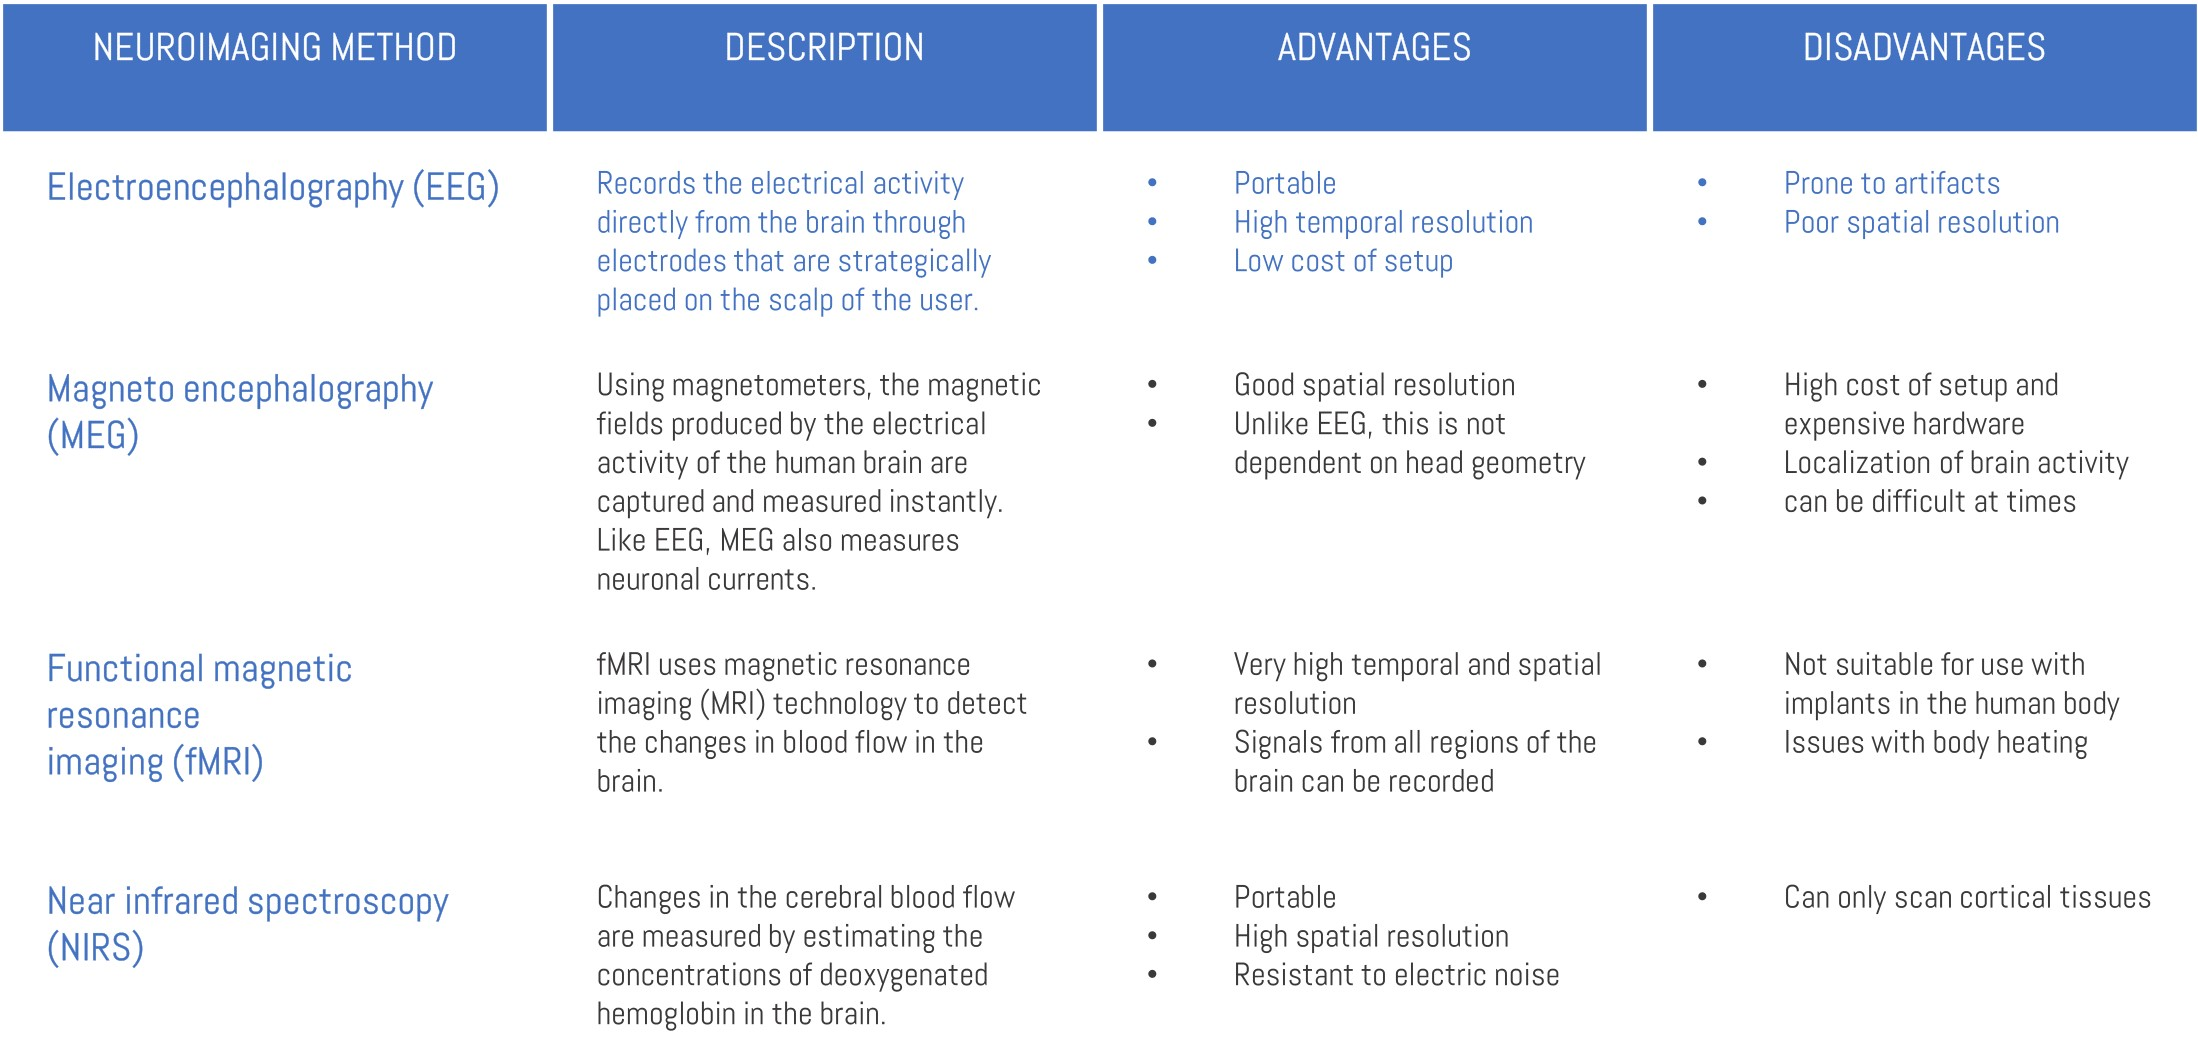
\includegraphics[scale=0.3]{fmri1.jpg}
\captionof{table}[Comparison of various neuroimaging methods]{Comparison of various neuroimaging methods \cite{bci_fs}}
\label{img:imaging_dev}
\end{figure}

\subsection{Electroencephalography}

Electroencephalography measures the electrical activity generated by the activity of neurons in the human brain in voltages. EEG has been used for several decades, it provides excellent time resolution and it can take thousands of snapshots per second. One of the biggest strengths of this imaging method is the ease of signal acquisition, portability and the possibility for a noninvasive measurement. All these features make this method desirable for incorporating into BCI solutions. \cite{imotions_2017}

\subsubsection{EEG measurement}

\begin{figure}[h]
\centering
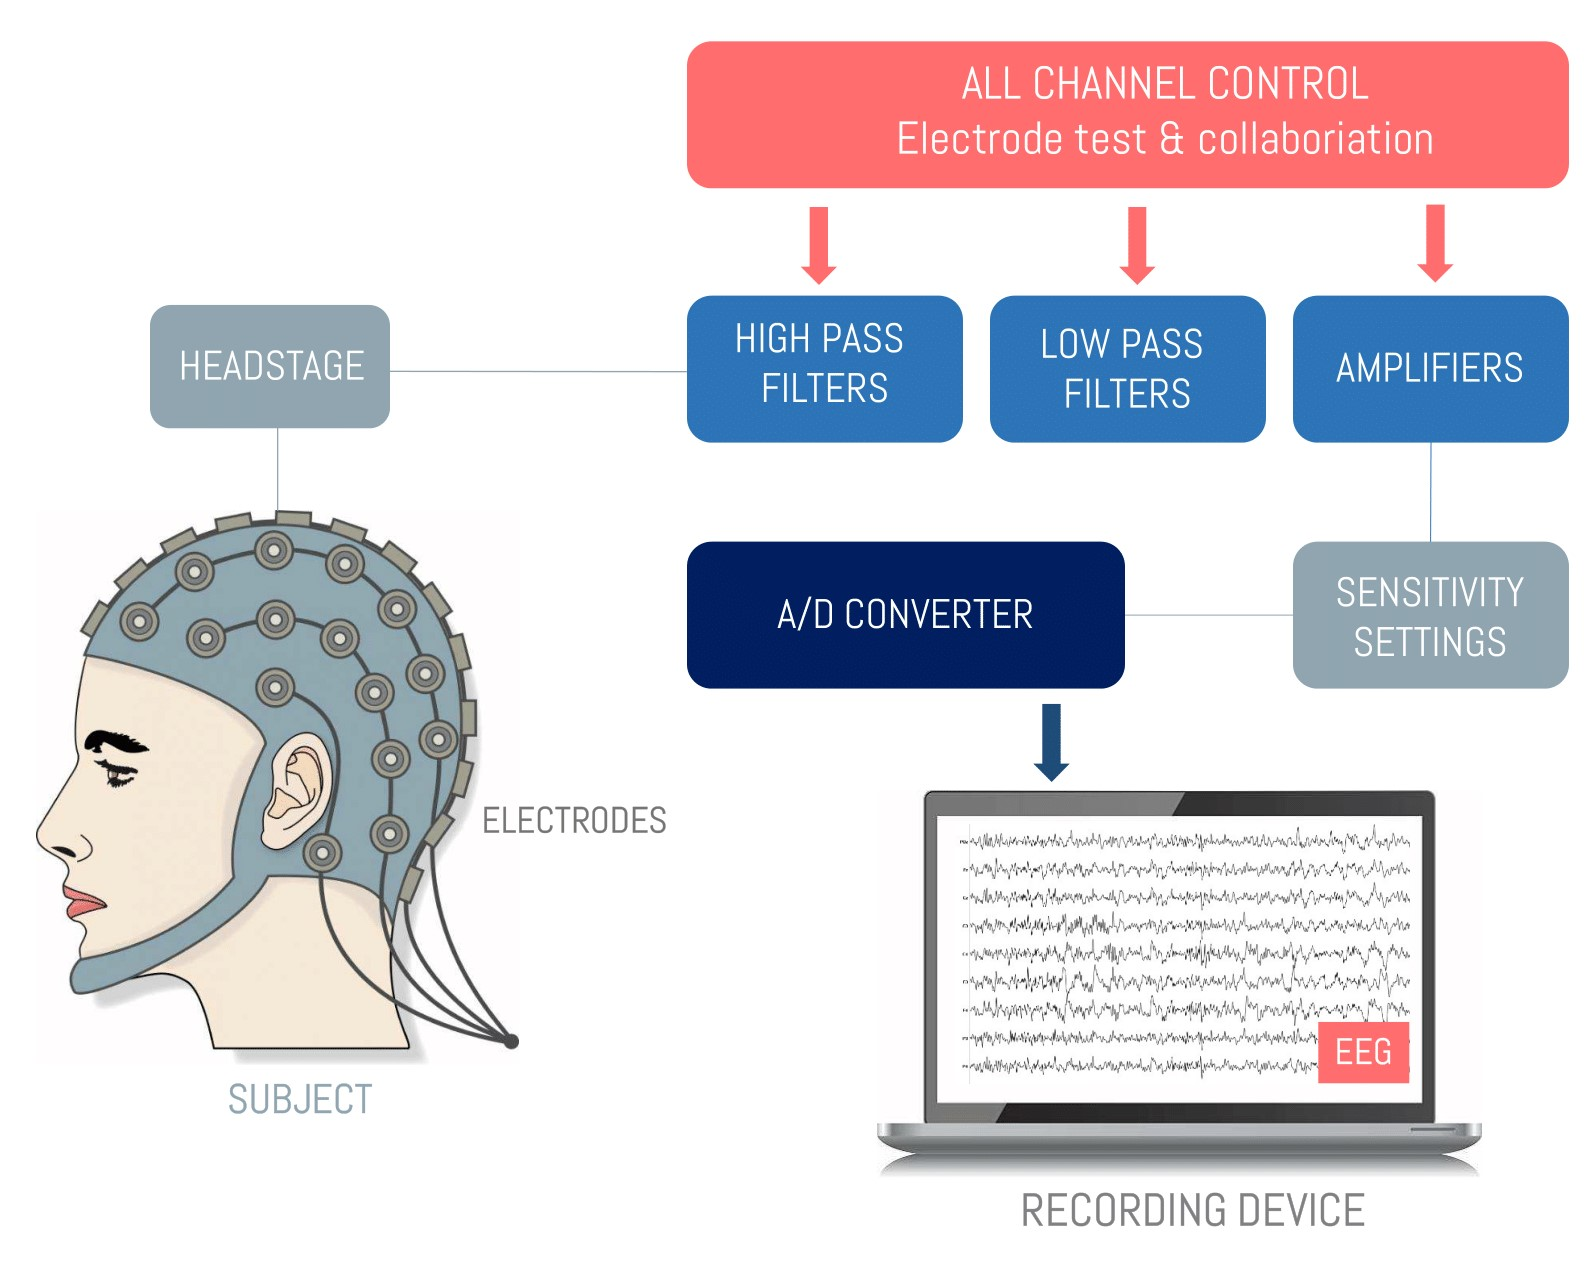
\includegraphics[scale=0.25]{eegabra.jpg}
\caption{Main elements of the electroencephalographic recording}
\label{fig:inside}
\end{figure}

The electroencephalographic recording device consists of the following elements:
\begin{itemize}
\item electrodes with conductive media
\item amplifiers with filters
\item A/D converter
\item recording device
\end{itemize}

Electrodes read the signal from the head surface - their well functioning is crucial for gaining high quality data for interpretation. The most widely used scalp electrode is the silver/silver chloride (Ag/AgCl) electrode, due to its excellent characteristics. They can record very slow potential alternations.
Neuronal activity recorded from the scalp allow measurement of potential changes over time in basic electric circuit conducting between the signal (active) electrode and the reference electrode. An additional third electrode (ground) is necessary for getting differential voltage (active - reference). \cite{teplan}
Figure \ref{fig:inside} shows the main components of the EEG measuring process: headstage, all channel control, high/low pass filters, amplifiers, A/D conversion and  recording device. 

\subsubsection{Signal analysis}

\paragraph{Amplifiers and filters}
In order to make the brain waves compatible with the A/D converter they need to be amplified, making sure to filter the desirable psychological signals from the noise and interference signals. The raw data consists of the valuable biopotentials, undesired biopotentials, interference signals generated by the human tissue, an 50/60 Hz interference (AC power line noise) and external noise.The desired signal appears between the 2 inputs of the differential amplifier. \cite{nagel}

\paragraph{Artifacts}
The artifact is recorded in with the desirable biopotentials and may be either patient-related or technical. Patient-related artifacts are unwanted physiological signals that may significantly disturb the EEG, such as any minor movements, electromyogram, electrocardiogram, eye movements and sweating. Technical artifacts are measurement related disturbances such as  AC power line noise, 50/60 Hz interference, cable movements and broken wire contracts.

From Mindtech's point of view one artifact holds the information, the blinking signal that represents the only communication between a LIS patient and the environment. There is a specific appearance of the signal, which can be extracted efficiently from the rest of the data. We can see an example of a typical blinking signal characteristic in Figure \ref{fig:blink}.

\begin{figure}[h]
\centering
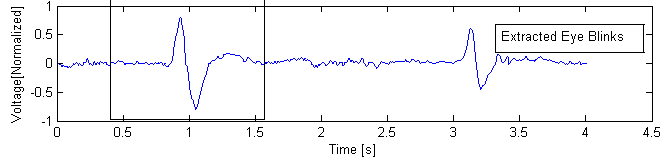
\includegraphics[scale=0.7]{blink.png}
\caption[Identifying the blinking signal from the raw EEG]{Identifying the blinking signal from the raw EEG \cite{matiko_beeby_tudor_2013}}
\label{fig:blink}
\end{figure}

\subsubsection{Brainwave classification}

Sinusoidal brain waves are measured from peak to peak, usually ranging from 0.5 to 100 µV in amplitude. These are categorized into four basic groups, related to specific activities of the patient. Delta waves (< 4 Hz) are occurring during deep sleep, Theta waves (4 - 8 Hz) are representing memory encoding and retrieval, Alpha waves (8 - 12 Hz) are typical patterns of relaxation and Beta waves (12 - 25 Hz) are occurring during attentive focusing. In Figure \ref{fig:class} we can see the most typical brain patterns of the frontal lobe and their functions.

\begin{figure}[h]
\centering
\begin{minipage}{.5\textwidth}
  \centering
  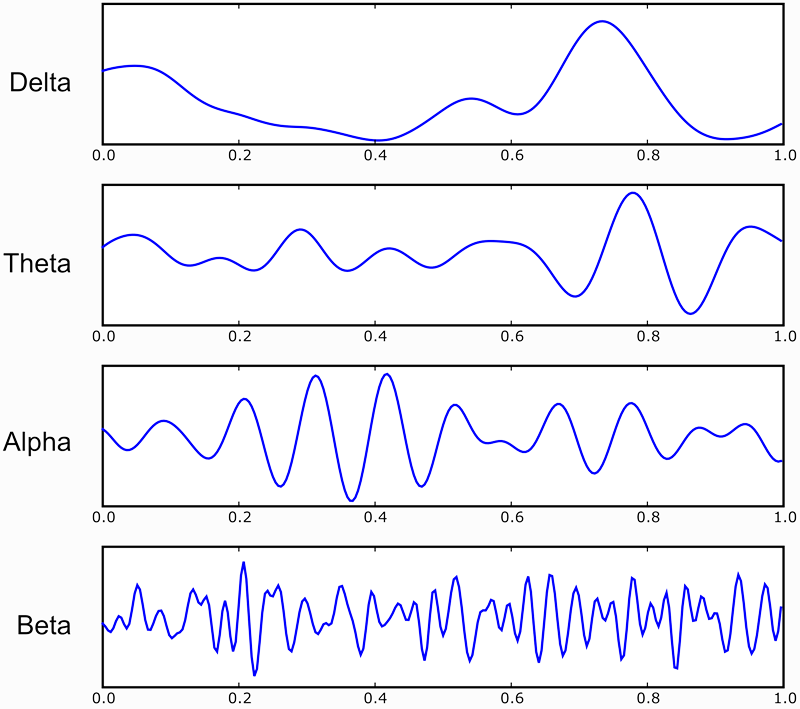
\includegraphics[width=0.8 \linewidth]{freq_bands.png}
\end{minipage}%
\begin{minipage}{.5\textwidth}
\begin{itemize}
    \item \textsc{delta} : < 4 Hz - deep sleep 
    \item \textsc{theta} : 4 - 8 Hz - memory encoding and retrieval
    \item \textsc{alpha} : 8 - 12 Hz - relaxation (appears at eye closure)
    \item \textsc{beta} : 12 - 25 Hz - attentive focusing
\end{itemize}
\end{minipage}
\caption[The typical EEG patterns of brain activity]{The typical EEG patterns of brain activity and the frequency bands they appearat \textit{http://econtact.ca}}
\label{fig:class}
\end{figure}


\subsubsection{Current devices, sensors}

There are a lot of non-invasive sensors out the market that use different approaches to measure EEG signals, from single channel to multi-channel solutions. Based on the point of measurement, the registered cortical activity can vary. For example different cognitive information can be derived from the frontal lobe and the parietal lobe.
The most popular and accessible measurement tools are summarized in the Table \ref{img:sensors}. Most of the solutions involve a multi-channel sensors (EPOC+, UltraCortex, Startism R20) which needs qualified assistance to conduct the measurement. The more simple products (BrainBandXL, Muse, NeuroSky) are ideal for everyday use, becuse they are adjustable and look more like a headset than a medical device. EPOC+, NeuroSky, Startism  and BrainBandXL headsets are ideal for measuring attention and meditation levels in a way that can be utilized for ADHD trainings.

\begin{figure}[!htbp]
\centering
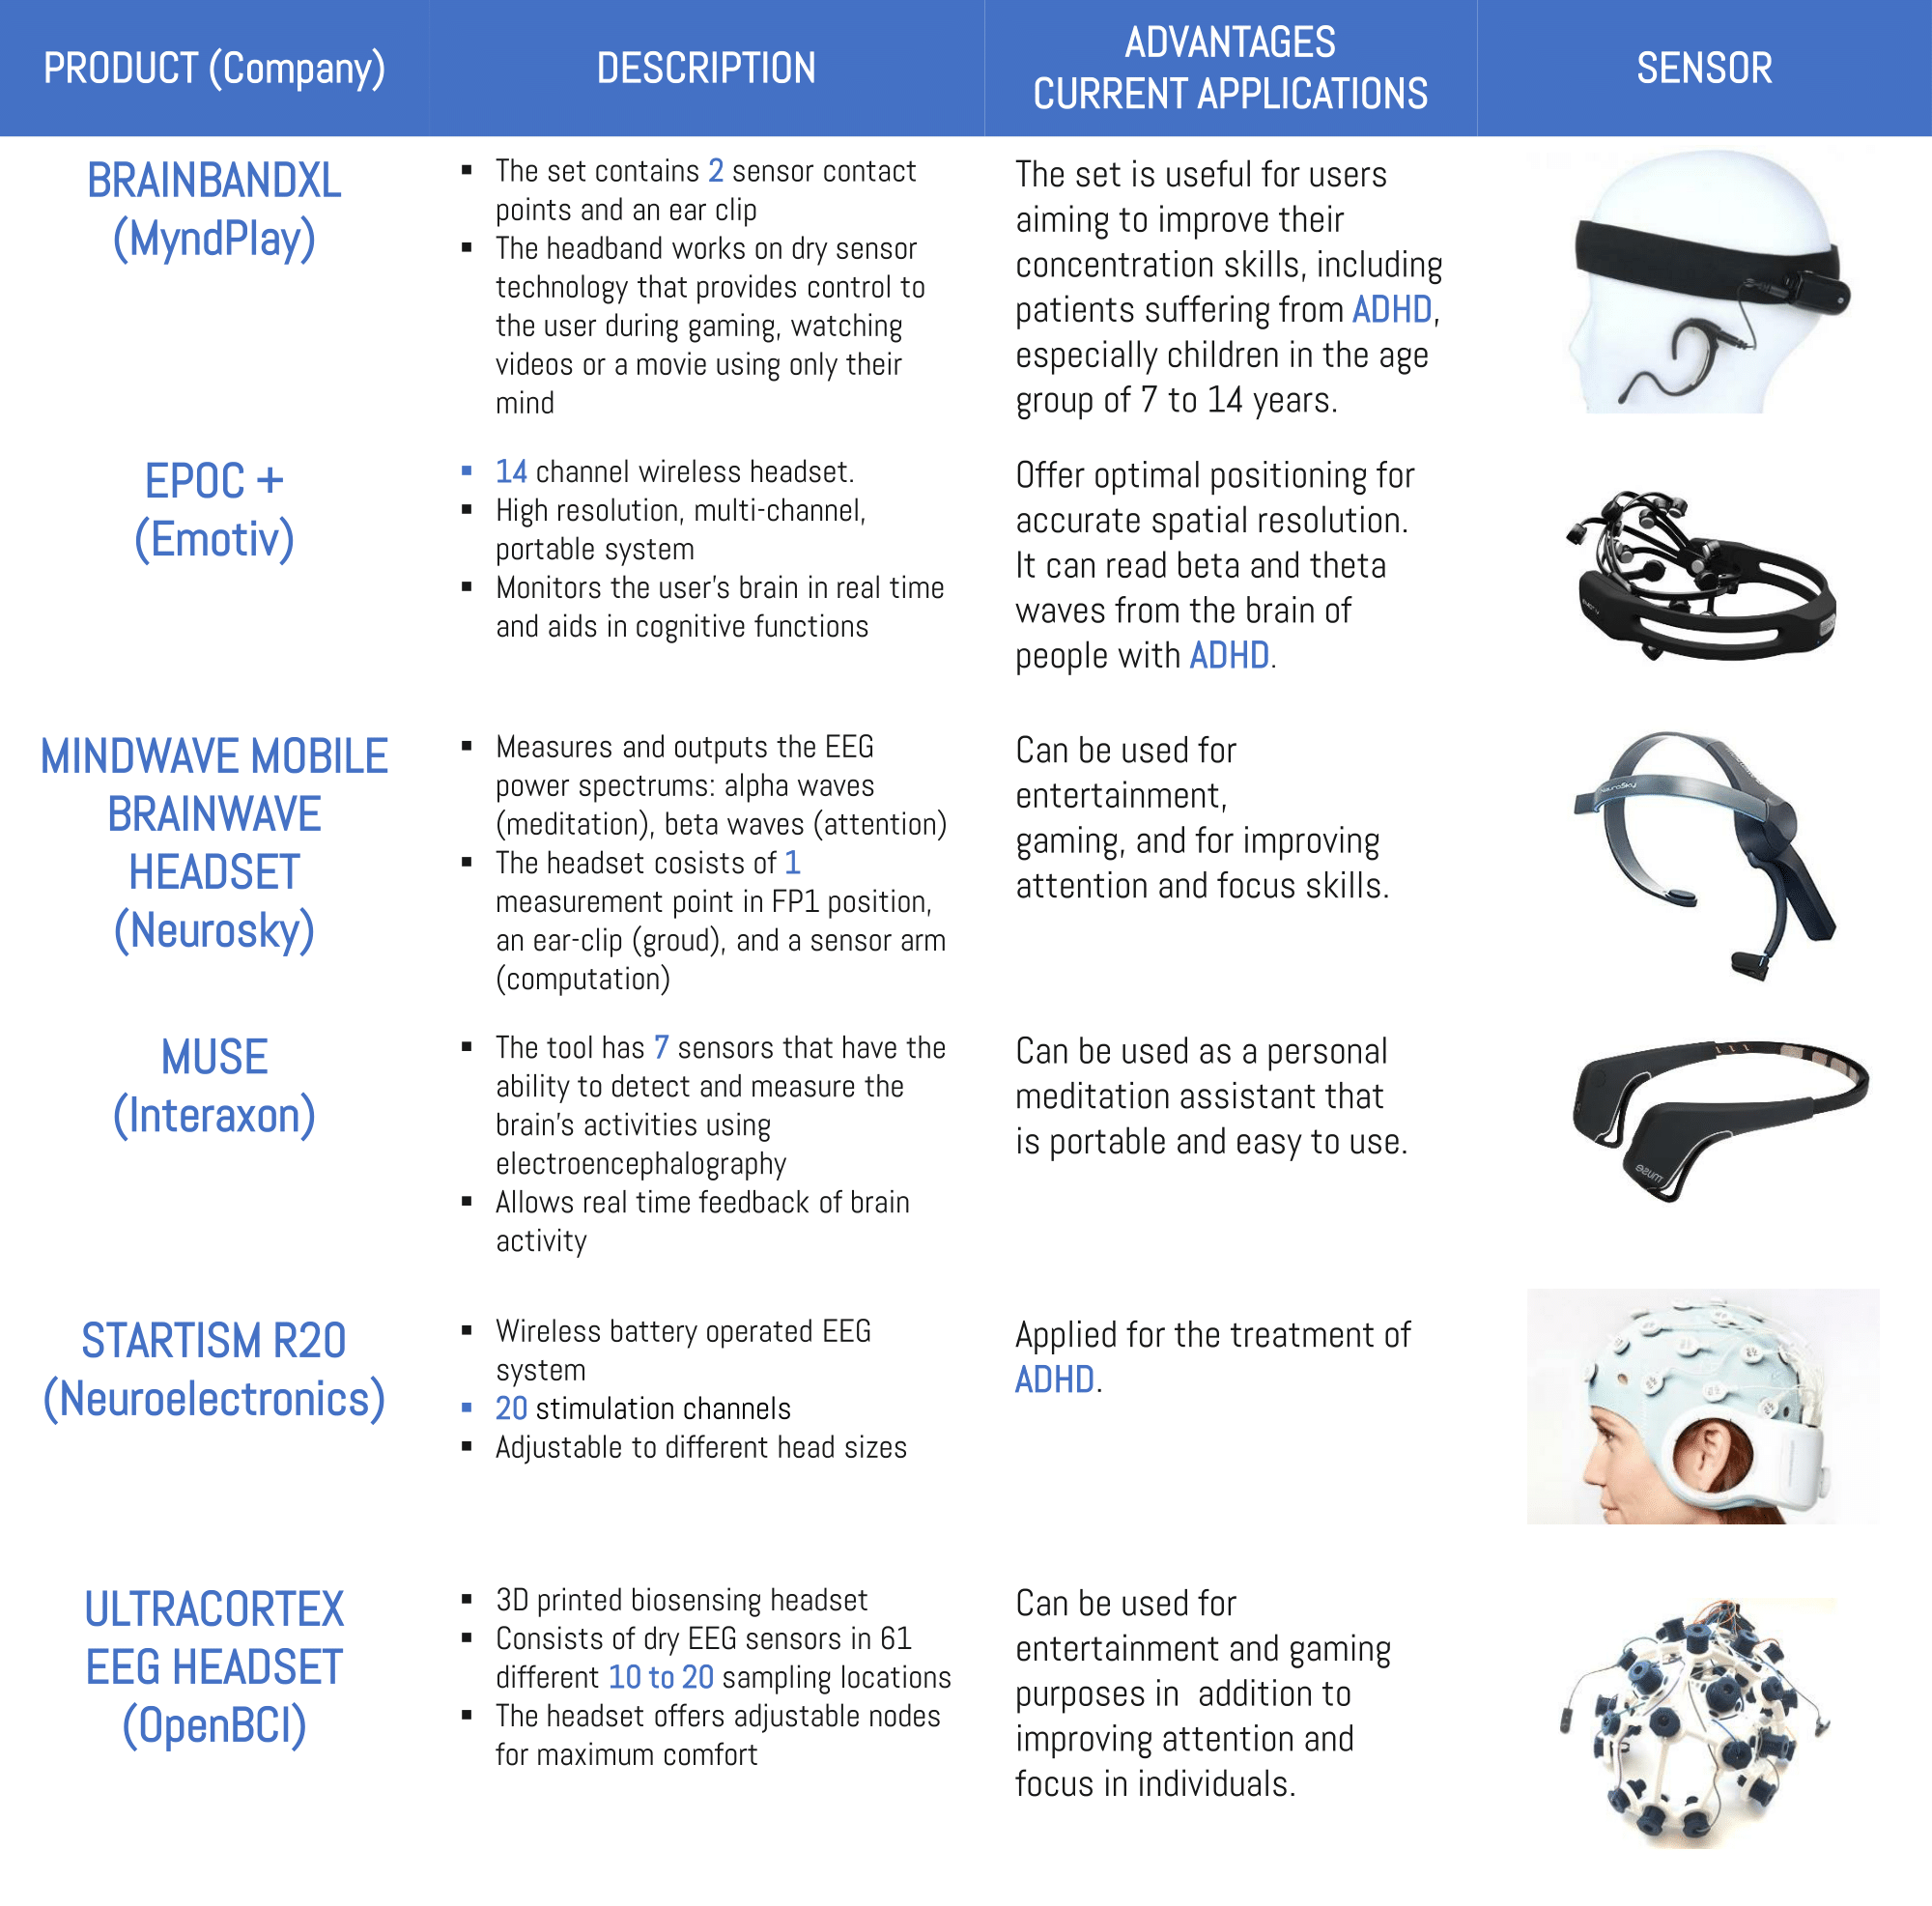
\includegraphics[scale=0.262]{sensors.png}
\captionof{table}[Comparison of various non-invasive EEG sensors]{Comparison of various non-invasive EEG sensors \cite{bci_fs}}
\label{img:sensors}
\end{figure}

\subsection{Technology approaches to the problems}

The following section will focus on the current and forecast technology solutions for AHDH, locked-in syndrome and driver attention monitoring markets.

\subsubsection{Technology solutions for ADHD}


We can extend the possible ADHD training list with neurofeedback training, which is a cognitive training for working memory, attention,executive functioning, and organizational skills. There are several software solutions for neurofeedback, some of them including BCI headsets as well.

Through a therapy session neurofeedback can be used to improve cognition, memory, speech skills, and pain management associated with a disease. One form of neurofeedback training utilizes two electrodes on the scalp and one on the earlobe that are placed during training sessions. By watching a display on the computer screen, the training sessions teach the person to slowly retrain their brainwave pattern. Ih as many as 15-20 sessions for treating anxiety and over 40 sessions for ADHD, neurofeedback can help treat complex conditions. \cite{bci_fs}

There are several EEG software packages on the market utilizing attention and meditation levels measured from the frontal lobe to get a clear insight on the patient's cognitive level. Solutions may include additional eye tracking, EMG, ECG and facial expression measurements. I give a detailed overview on these solutions after introducing Mindtech's technlogy.


\subsubsection{Technology solutions for Locked-In Syndrome}

There are several studies devoted "unlocking" the LIS patients, ranging from the classic, incomplete and total presentations. The most difficult case to deal with is the total locked-in syndrome, where the patient is completely paralyzed, without any eye-movements. In this case the scientists use functional magnetic resonance (fMRI) imaging combining with electrocorticography (ECoG), which is an invasive method.  

Besides invasive embedded BCI chips, there is much work being done to create an effective non-invasive solution for total LIS patients. NeuroSky developed its own sotfware called MindScribe, which uses the NeuroSky headset as well. The usage of the device hard to learn and the patient has to concentrate hard to gain results. Three different modes of communication is possible with the device: identification of emotional state, yes/no response and a typing mode. The device is mostly targeted for use by complete locked-in patients. 
\cite{mannes_2016}


Patient-computer interfaces such as infrared eye movement sensors and computer voice prosthetics are being further developed by rehabilitation engineers and speech language therapists. \cite{smith_delargy_2005}

At Northeastern University a group of electrical and computer engineers developed a new eye tracking technology, using electrodes positioned on the two sides of the face close to the eyes. They measure voltage differentials based on the electrodes polarity, when the eyes are moving left or right. When the user is looking at the screen with a keyboard, they can select a specific letter with blinking. The device allows users to type out messages to their loved ones and care givers. \cite{neu}

A company called LC Technologies is manufactures several eye tracking systems, mostly targeted for ALS patients, but can also provide a bridge in communication for pateints with LIS as well. Eyegaze Edge Tablet and Eyegaze Edge Desktop are both monitors that come in different sizes, with a touch pen, keyboard, and with high speed infrared camera and lens. The system has it's own communication software, enabling the user to send emails and browse the internet with eye tracking. \cite{yusuf}


\subsubsection{Technology solutions for driver attention monitoring}

According to a Frost & Sullivan market report, drowsiness detection and eye tracking are the basic features that OEMs are looking to commercialize by 2018. Camera-based Driving Monitoring Systems are expected to be introduced on the market by the end of 2017. \cite{f&s_car}  Many car manufacturers are working on the implementation of different sensors, to provide a DMS in their models. The forecast of the different identification features implemented into passenger cars are summarized in Table \ref{fig:cars}. In the last row we can see how brain wave detection is expected to be the part of the DMS, but only two companies (Jaguar and Mercedes) are planing to introduce the system in the near future (2022).

\begin{figure}[h]
\centering
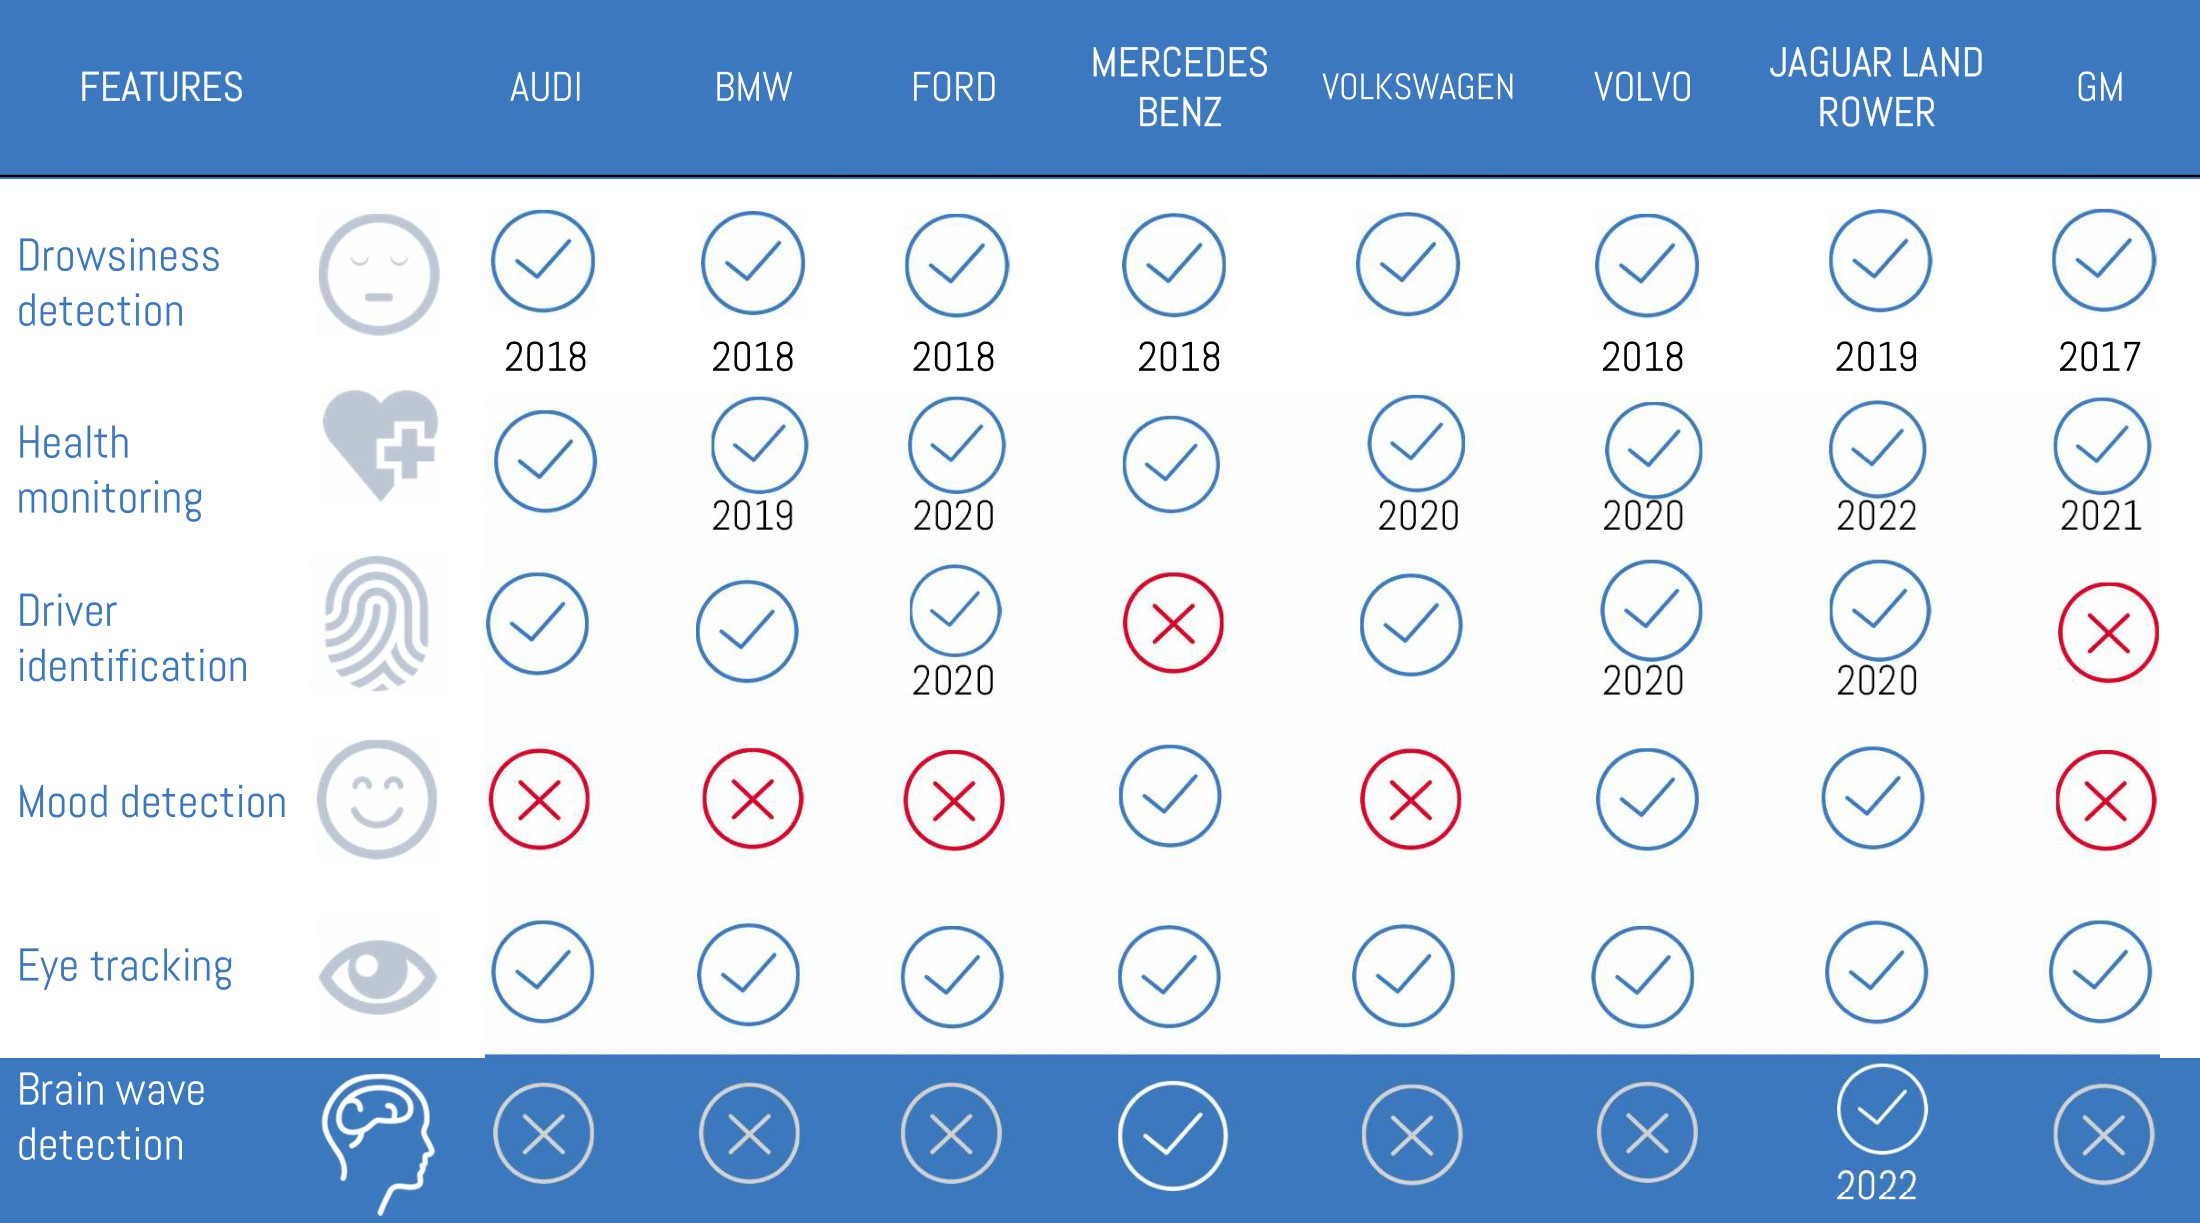
\includegraphics[scale=0.26]{dms.jpg}
\captionof{table}[Forecast and overview of different car manufacturers implementing DMS solutions in their new models.]{Forecast and overview of different car manufacturers implementing DMS solutions in their new models. \cite{f&s_car}}
\label{fig:cars}
\end{figure}


As Table \ref{fig:cars} has already summarized, there are car manufacturers already aiming to provide solutions for increasing driver alertness. An example of these solutions is the product of a company called Plessey, who is commercializing a sensor for driver attention monitoring called the WARDEN™, a new heart-rate based driver alertness monitoring system. They are using a sensor called EPIC™ (Electric Potential Integrated Circuit), which can provide the necessary biometric signals and provide earlier warning of drowsiness or health issues.
\cite{plessey}



\subsubsection{Weaknesses of the current technology solutions}

\paragraph{ADHD} Most of the neurofeedback solutions are location dependent and expensive. The frequency of visits to the hospitals, training centers and private therapists providing these trainings are not enough to result in long-term results.

\paragraph{Locked-in syndrome}The family of a patient suffering from locked-in syndrome can easily spend \$15,000 on eye tracking devices, which are in most cases hard to use for LIS patients. The software NeuroSky is offering is around \$1,500, which is still a high price for most of the affected families. Mindtech is offering a solution which is accessible for everyone with it's on a blink based technology. It is easy to learn and train for the users profile and even patients with very weak blinking capabilities can use it.

\paragraph{Driver Alertness}There are several challenges with the currently available monitoring possibilities. Camera based solutions fail to work in all lightning conditions, it is hard to place a camera to suit different drivers and eye detection is harder when the driver wears glasses or sunglasses. Furthermore, placing biosensors inside the seat, on the steering wheel, or on the seat belt is expensive and needs for improvements as well.  \cite{f&s_car}



\subsection{Mindtech's technology principles}

\subsubsection{Core elements}

Mindtech choose to use the NeuroSky Mindvawe Mobile headset to collect real time brain wave data from the users. They combine this technology with Android/iOS development and all the applications coming from this process are accessible for devices from smart phones to tablets. All these features make Mindtech's technology portable (the headsets main characteristic), flexible and easily spreadable.


\subsubsection{NeuroSky headset}

NeuroSky has been working on electroencephalography (EEG) and electromyography (EMG) technologies since 2004, and it produces Brain-Computer Interface technologies for consumers. The company uses low-cost EEG-linked dry sensors. They products are accessible for everyone in a price range of \$80-\$130. The MindWave mobile headset is created for a wide range of purposes, including education fitness, entertainment  and research/development. \cite{wearable} The measuring headset, with its own built-in computational device, has incredible advantages. The MindWave mobile headset is compatible with personal computers, Mac, iPad and mobile devices running on iOS and Android. \cite{neurosky} Figure \ref{fig:headsetcomponents} shows the main part of the device: adjustable head band, sensor tip/arm, flexible ear arm, ear clip, battery are and power switch.

\paragraph{Features of the device}

\begin{figure}[h]
\centering
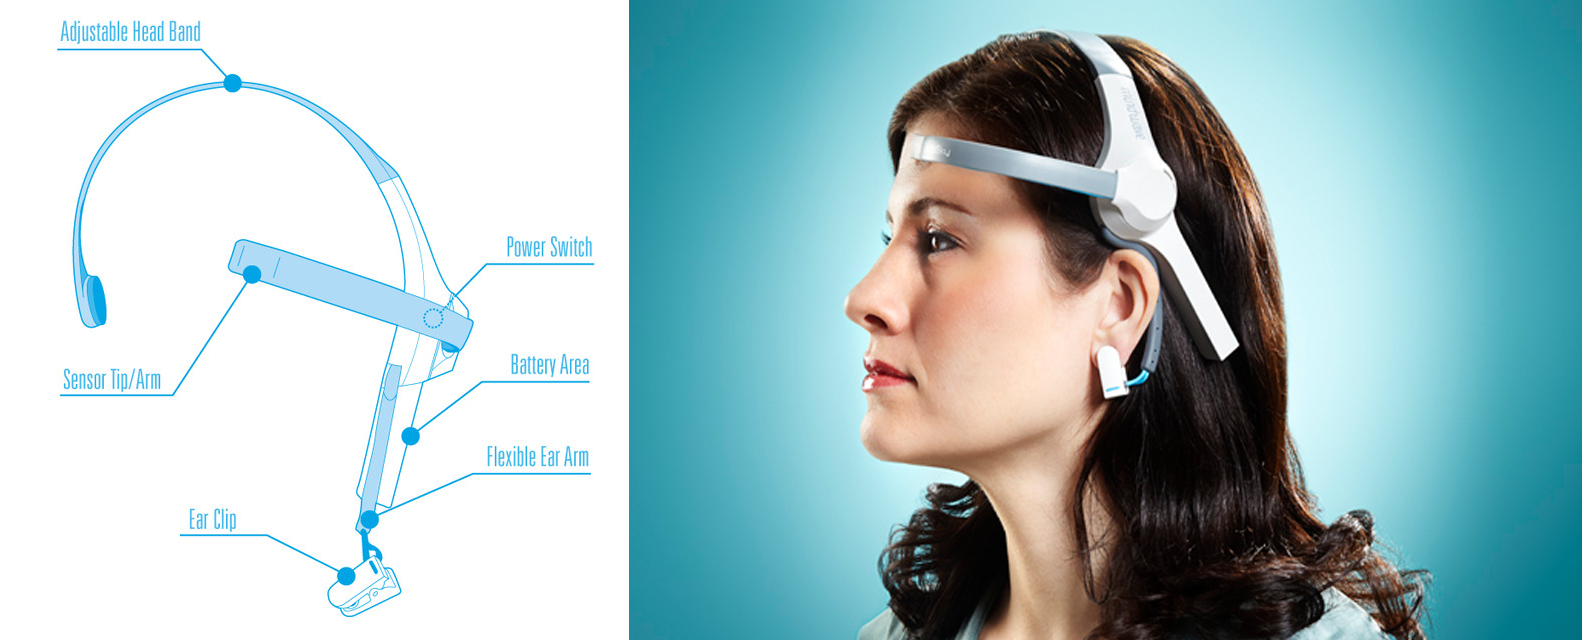
\includegraphics[scale=0.5]{mindwave.png}
\caption[Outside components of the NeuroSky MindWave Mobile headset]{Outside components of the NeuroSky MindWave Mobile headset \textit{© NeuroSky}}
\label{fig:headsetcomponents}
\end{figure}

The EEG measuring sensor comes in form of a headset, which is both comfortable to wear and easy to properly position on the head. The main parts of the device are: a flexible \textbf{headband}, a measuring point in the form of an \textbf{electrode}, that is extended in a way so that the \textbf{sensory tip arm} reaches the FP1 point on the forehead, the  \textbf{reference + ground}, embedded in an \textbf{ear clip}, which is easy to apply, and the \textbf{computational module} situated closely to the \textbf{battery} area. The device can be turned on/off with a \textbf{power switch}.

The portable EEG brainwave headset has 6-8 hours battery run time (working with a  AAA battery), has safe passive biosensors, it is lightweight, and is capable of automatic wireless computer pairing.  \cite{neurosky}

\paragraph{Hardware Overview}

The headset consists of three main functional components: electrode, ground and the ThinkGear AM module. The inside components of the headset can be examined in Figure \ref{fig:inside}, particularly focusing on the TGAM module characteristic with the TGAT chip inside.

\begin{figure}[h]
\centering
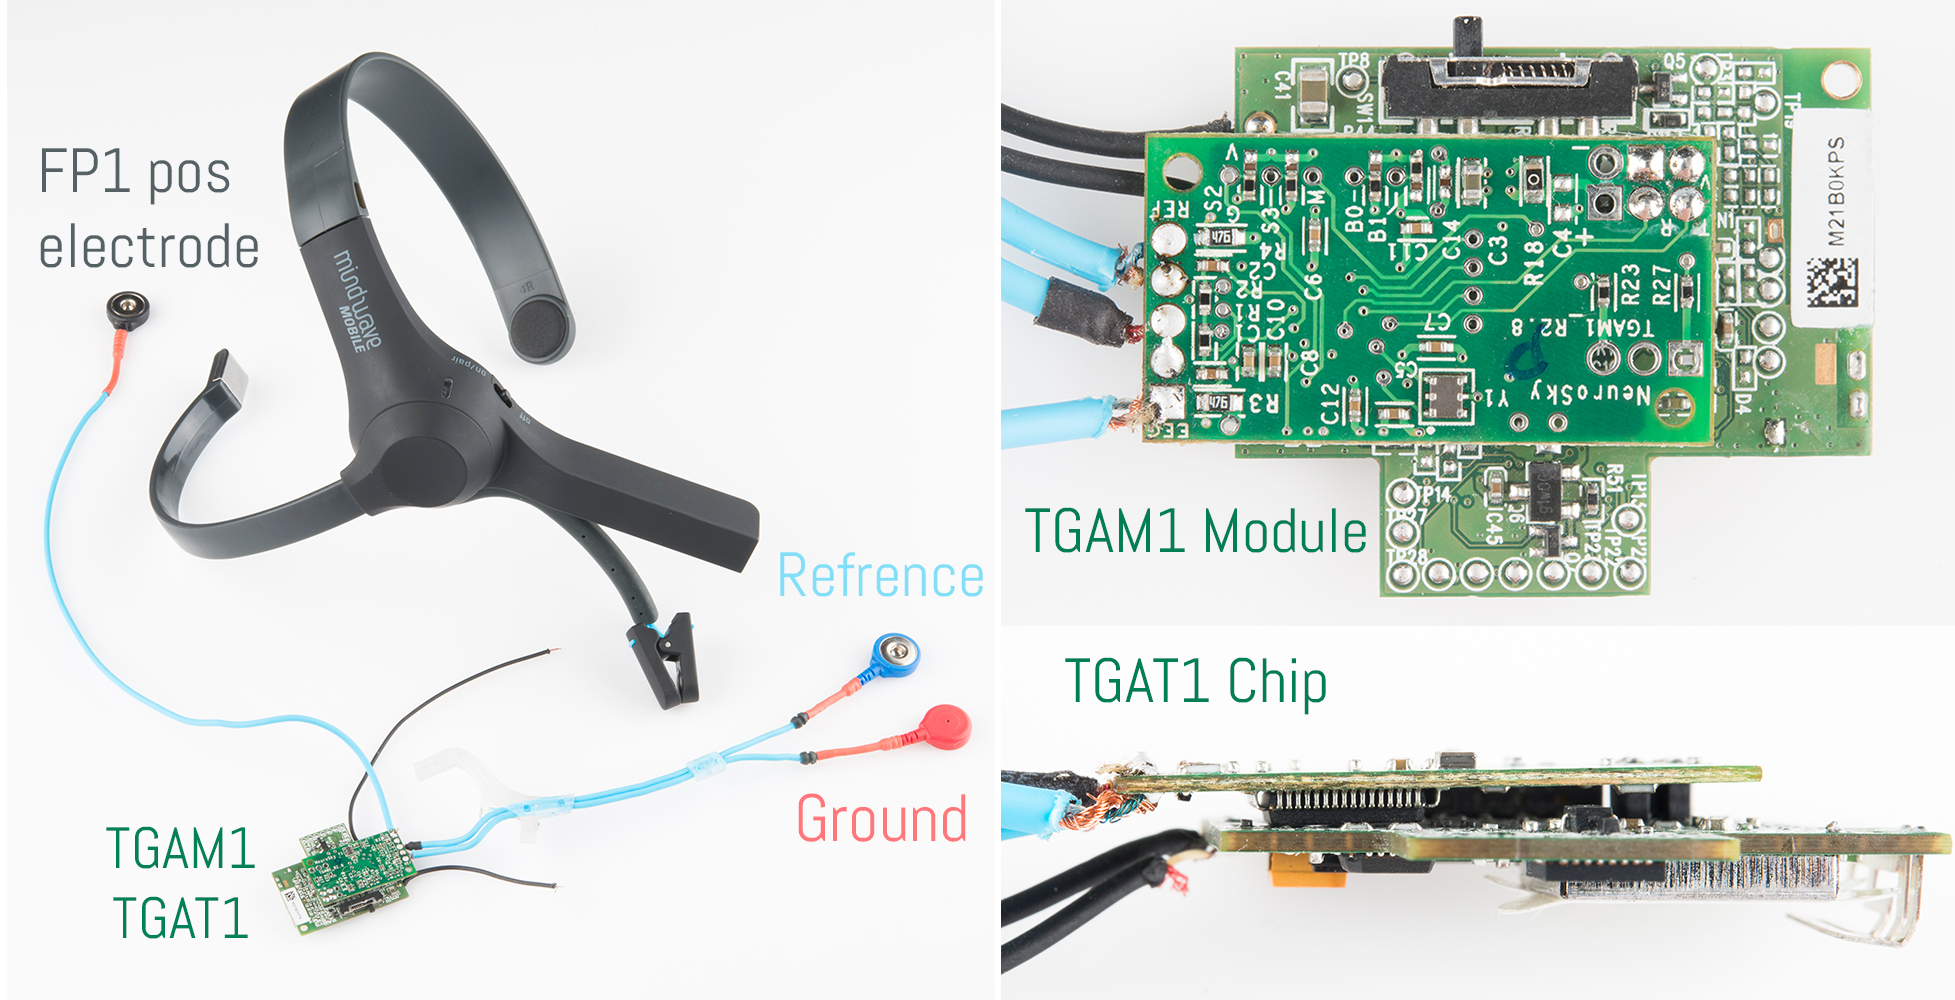
\includegraphics[scale=0.7]{hardware.png}
\caption[Hardware components NeuroSky MindWave Mobile headset]{Hardware components NeuroSky MindWave Mobile headset \textit{Parts taken apart by Sparkfun}}
\label{fig:inside}
\end{figure}

\subparagraph{Electrode} The Device has only one measuring point in the FP1 position with a dry stainless steel electrode. This EEG channel provides a good temporal resolution about the frontal lobe activity, measuring alpha and beta oscillations and muscular signals from eye movements. More characteristics of the electrode can be seen in Figure \ref{fig:electrode}.

\begin{figure}[h]
\centering
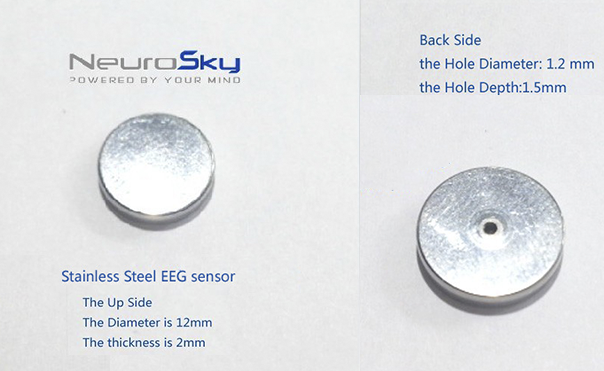
\includegraphics[scale=2]{neuroskjy.png}
\caption[Dry electrode characteristics from the NeuroSky MindWave Mobile headset]{Dry electrode characteristics from the NeuroSky MindWave Mobile headset \textit{© NeuroSky}}
\label{fig:electrode}
\end{figure}

\subparagraph{Reference and ground}
The ground is has to responsibility of prevents the power line noise from interfering with the small biopotential signals of interest. The measured electrical potential differences are the voltage drops from the active electrode to the reference electrode. \cite{biopac}
The positioning of the NeuroSky headsets electrode system is reconcilable with the international 10-20 electrode placement, presented in Figure \ref{fig:electrodeplacement}.

\begin{figure}[h]
\centering
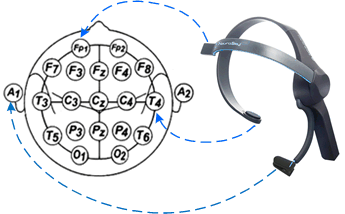
\includegraphics[scale=0.6]{positioning.png}
\caption[Position of MindWave Mobile headset electrodes on 10-20 international system of electrode placement]{Position of MindWave Mobile headset electrodes on 10-20 international system of electrode placement \cite{matiko_beeby_tudor_2013}}
\label{fig:electrodeplacement}
\end{figure}


\subparagraph{ThinkGear ASIC Module}

ThinkGear AM Module (TGAM) is the heart of computational power within the NeuroSky MindWave mobile sensor and the brainwave sensing technology. Within the TGAM there is a ThinkGear ASIC chip (TGAT), which is a powerful, fully integrated single chip EEG sensor. The chip is capable of computing the scale of attention and meditation from the beta and alpha brainwaves, and it can detect blinks, from eye muscle movement signals. The chip is capable of processing 5 different types of brain oscillations. \cite{neurosky}


\paragraph{Software Overview}

The TGAT chip is already programmed with NeuroSky eSense (EEG algorithm package), analog to digital converter (A/D), amplification off head detection, noise filtering for electromyogram artifacts, and 50/60 Hz AC powerline interference. \cite{neurosky}

The NeuroSky MindWave mobile provides the following outputs for the user: 
\begin{itemize}
\item Raw EEG signal
\item Delta, theta, low alpha, high alpha, low beta, high beta, gamma waves
\item Attention
\item Meditation
\end{itemize}

The device comes with built in EEG algorithms for the attention, meditation and blink detection measurements.

The \textit{Attention Meter algorithm} indicates the intensity of mental focus or attention, scaled on a range from 0 to 100. The level of attention increases when a user focuses on a single thought or an external object, and decreases when the user gets distracted from it. \cite{neurosky}

The \textit{Meditation Meter algorithm} measures the level of mental relaxation. The range is from 0 to 100, increasing when the user is more relaxed and decreasing when the user is disturbed or stressed. \cite{neurosky}

The \textit{Blink Detection algorithm} is capable of detecting the user's blinks and characterizing it with a number. A higher value means a stronger blink, while a smaller value describes a lighter blink. \cite{neurosky}


\paragraph{Positioning among other sensors}

Most of the sensors presented in Table \ref{img:sensors} are used in either clinical or research environment, with professionals assisting in the measurement. Even an electrode cap is hard to position properly without assistance. In almost all cases the electrodes need to be soaked in gel or a liquid increasing the conductance. The process preparing to measure with multichannel sensors is circumstantial and requires assistance and practice.
However, the NeuroSky MindWave mobile headset is designed for everyday use, and does not require any assistance with the measurement. It measures brainwave signals and monitors the attention levels of students as they interact with math, memory, and pattern recognition applications. The MindWave headset is a plastic device which fits comfortably over the left ear. The primary sensor sits on the forehead. Before the measurement the surface have to be cleaned. The sensor works perfectly without using gel, although it takes a minute or two to adjust it the first time the user put it on. It connects via Bluetooth to the device. \cite{wearable}
It is a single channel headset, which allows it to gain data from the frontal lobe in order to measure the attention and meditation related brain activity from the best FP1 position. It is light weighted, easy to fit without any previous knowledge in EEG measurements, and it is the most affordable and trustworthy piece on the market.



\subsubsection{Application development}

The list of available Mindtech solutions and their target audiences can be found in Table \ref{fig:apps}. TrainDHD provides real time attention monitoring for the ADHD patient, measuring attention and meditation levels specific for a task. DriveAlert measures brain activity and  blinks to determine the level of alerntess of the driver. When the driver is not paying attention the app warns him to take a break. BlinkTyper was developed for locked-in syndrome patients and has a keyboard which can be controlled by blinking. The typed in text can be saved into a quick phrases list, to make to communication easier. A chosen phrase can be read out loud with the phone. LIS patients can control a pdf or ebook with single and double blink command signals with BlinkReader. MemoryBlink provides a rehabilitation option in form of a memory game for LIS patients in order to decrease the level of depression. The classic memory game can be controlled by blinking.



\begin{figure}[h]
\centering
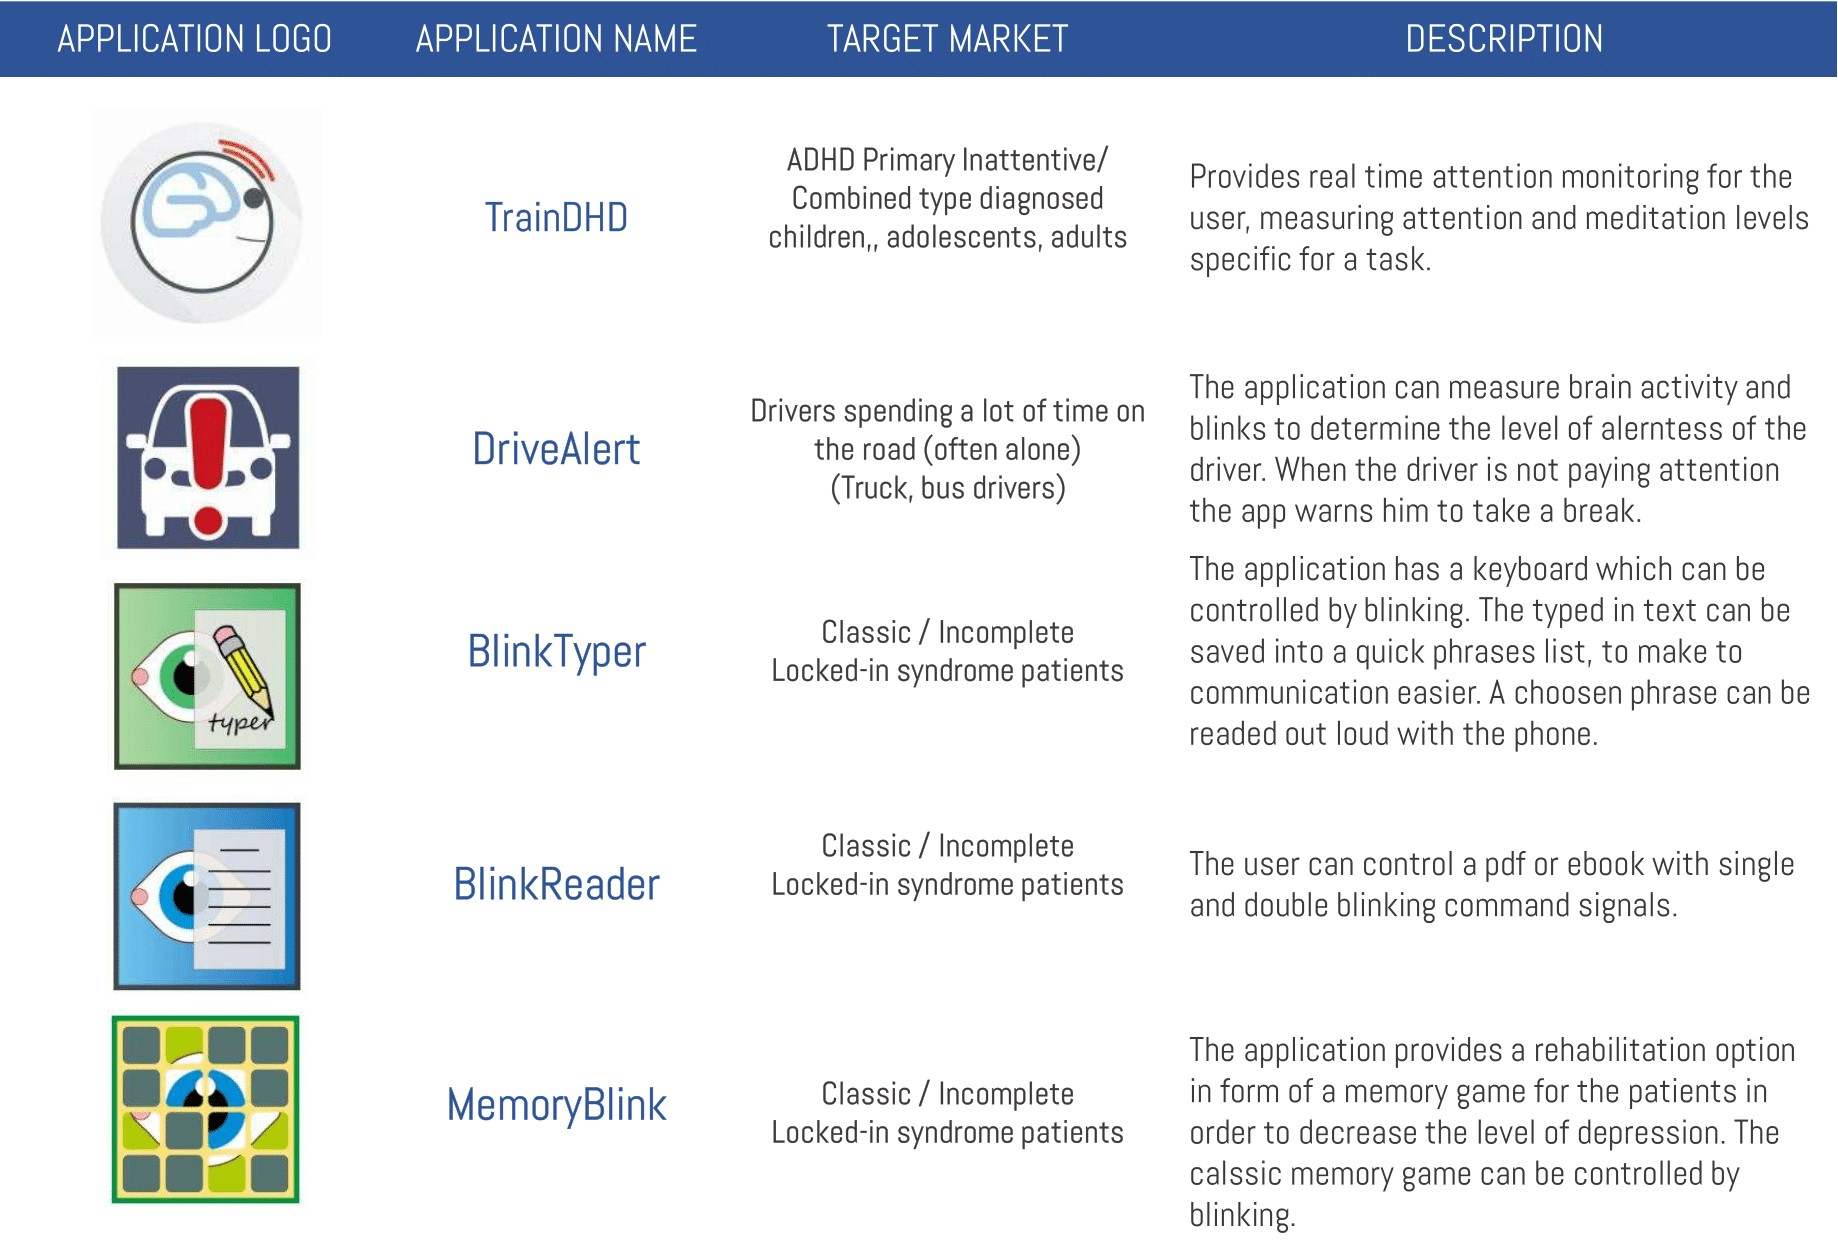
\includegraphics[scale=0.3]{apps.jpg}
\captionof{table}{Summary of Mindtech's available applications}
\label{fig:apps}
\end{figure}


\subsubsection{NeuroSky developer tools}

NeuroSky provides an accessible developer library, which is part of the ThinkGear framework. The company provides a software development kit (SDK) for Android and iOS operation systems, empowering programmers to use these technologies for innovative application development purposes. The headset communicates with a device with a Bluetooth connection, the Mindtech application gets the data from the headband through the NeuroSky SDK. The eSense algorithm running in the TGAT chip provides pre-processed signals, determining the current attention and mediation level of the patients, indicated with an integer number between 0 and 100. Lower values represent lower levels of concentration/relaxation, higher values mean higher levels of concentration/relaxation. The NeuroSky headset transmits the calculated values to a connected smart phone vie Bluetooth connection in every single second (1 Hz frequency).
Besides the attention level measurement, blink detection takes place at the level of TGAT chip. The eSense algorithm assigns an integer value from 0 - 100 to the intensity of the blink. The blink detection and the raw EEG data get transmitted with 512 Hz. \cite{neurosky3}

All the signals sent from the NeuroSky headset are summarized in Table \ref{fig:neuroskysignals}.

\begin{table}[h]
\centering
\caption{Signals sent from the NeuroSky headset}
\label{fig:neuroskysignals}
\begin{tabular}{lccc}
\multicolumn{1}{c}{\textbf{Name}}       & \textbf{Description}                                 & \textbf{Data type}                               & \textbf{Frequency}  \\ \hline
\multicolumn{1}{|l|}{MSG\_RAW\_DATA}    & \multicolumn{1}{c|}{raw EEG signal}                  & \multicolumn{1}{c|}{integer  {[}-32768,32767{]}} & \multicolumn{1}{c|}{512 Hz} \\ \hline
\multicolumn{1}{|l|}{MSG\_POOR\_SIGNAL} & \multicolumn{1}{c|}{signal quality}                  & \multicolumn{1}{c|}{integer {[}0,200{]}}         & \multicolumn{1}{c|}{1 Hz}   \\ \hline
\multicolumn{1}{|l|}{MSG\_ATTENTION}    & \multicolumn{1}{c|}{attention level}                 & \multicolumn{1}{c|}{integer {[}0,100{]}}         & \multicolumn{1}{c|}{1 Hz}   \\ \hline
\multicolumn{1}{|l|}{MSG\_MEDITATION}   & \multicolumn{1}{c|}{meditation level}                & \multicolumn{1}{c|}{integer {[}0,100{]}}         & \multicolumn{1}{c|}{1 Hz}   \\ \hline
\multicolumn{1}{|l|}{MSG\_BLINK}        & \multicolumn{1}{c|}{detected blink intensity}        & \multicolumn{1}{c|}{integer {[}0,100{]}}         & \multicolumn{1}{c|}{512 Hz} \\ \hline
\multicolumn{1}{|l|}{MSG\_EEG\_POWER}   & \multicolumn{1}{c|}{complete EEG frequency spectrum} & \multicolumn{1}{c|}{integer {[}0,100{]}}         & \multicolumn{1}{c|}{1 Hz}   \\ \hline
\end{tabular}
\end{table}


\paragraph{Android environment}

Tamas Kralik, the CEO of Mindtech, developed a custom Android service which provides a framework for the communication between the NeuroSky MindWave Mobile headset and the smart phone. This service can be modified to all three Mindtech solutions, and enables the developers to get attention, meditation and blink related values from the device.

All three Mindtech solutions (TrainDHD, Blink - Reader, Writer, Memory game package, Drive Alert) are developed in Android Studio, an integrated development environment and tested on a Android smart phones and tablets.

All the applications are built  up from modular subsets and hold different functions. Activities, Helper Methods, Objects, and Services are the core elements of the application.

\paragraph{Structure of the application}

\subparagraph{Activity} The class Activity is the most important building block of any Android application. The class contains a user interface (UI) and a code controlling the UI. The Activity has 2 parts: the XML layout file behind the UI, and the Activity.class Java file behind the function of the interface. The Activity can be corresponded to a certain screen content in the application. The life cycle of the Activity is summarized in Figure \ref{img:activity}. 


\begin{figure}[h]
\centering
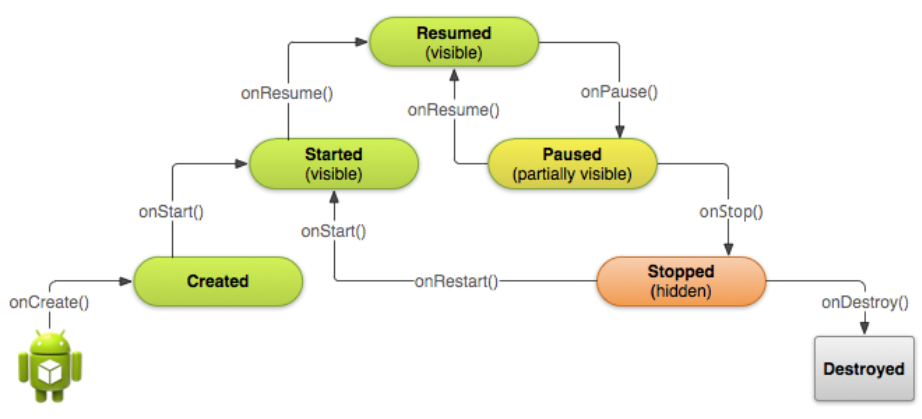
\includegraphics[scale=0.4]{android.PNG}
\caption[The flowchart representing the life cycle of the Activity class]{The flowchart representing the life cycle of the Activity class \cite{develop}}
\label{img:activity}
\end{figure}

\subparagraph{Layout} The Layout is an XML file describing the whole user interface. This file contains all the elements visible on the screen and their characteristics. The screen design can be done from code, or with a GUI in Android Studio design platform. 

\subparagraph{Service} The Service is a component running in the background, responsible for maintaining the Bluetooth connection with the headset.


\subsubsection{Prototype review}


\paragraph{Attention control application for ADHD}

TrainDHD consists of the following Activities, presented on the Figure \ref{img:prototype}. 

\begin{figure}[h]
\centering
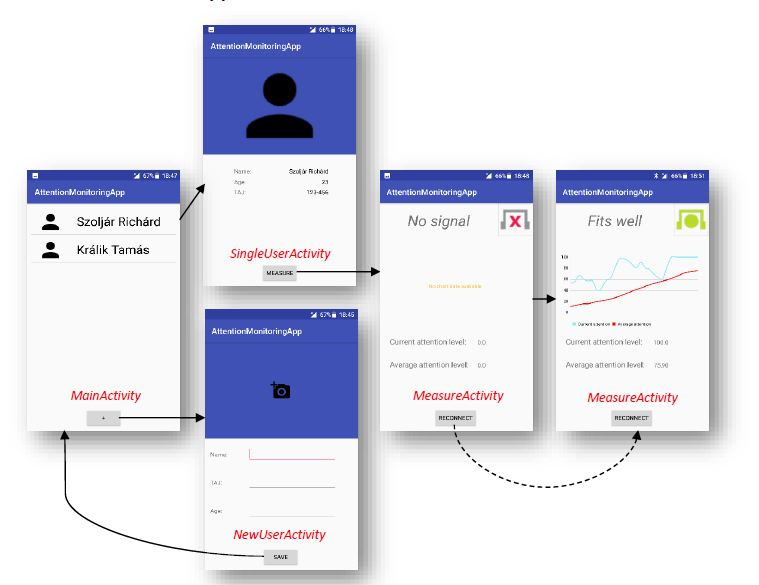
\includegraphics[scale=0.5]{prototype.JPG}
\caption[Structure of the application and the name of the activities depicted by red labels]{Structure of the application and the name of the activities depicted by red labels \cite{RicsiSzakdoga} }
\label{img:prototype}
\end{figure}

\subparagraph{MainActivity}
The first activity is the so called MainActivity, which appears when the user opens the application. In this activity one can see the name and the optionally selected thumbnail image of every single patient. \cite{RicsiSzakdoga}

\subparagraph{NewUserActivity}
When the user touches the plus button in the MainActivity, a new activity opens (called NewUserActivity) where they can fill in the text boxes in order to add necessary personal information about the new patient. \cite{RicsiSzakdoga}

\subparagraph{SingleUserActivity}
The SingleUserActivity is an activity which appears when the user touches one of the listed patient's names in the MainActivity. In this activity one can see the previously given personal information. The user can start the attention monitoring process from this activity by clicking the measure button at the bottom of the screen, which will open the MeasureActivity. \cite{RicsiSzakdoga}

\subparagraph{MeasureActivity}

The MeasureActivity is the activity where the attention level is measured, with the help of the NeuroSky MindWave Mobile EEG headset. It handles the communication and data acquisition processes from the NeuroSky headset with the utilization of the previously mentioned Android framework. Each second it receives an integer number between 0 and 100 from the EEG device which represents the current attention level of the patient who wears the NeuroSky headset. These values are then dynamically plotted in a line chart which provides a real-time feedback to the special education teacher about the attention level of the patient. \cite{RicsiSzakdoga}
The attention level is monitored on the screen as illustrated on Figure \ref{img:attention}.


\begin{figure}[h]
\centering
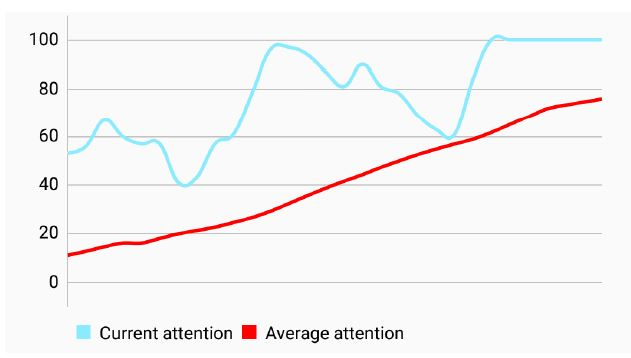
\includegraphics[scale=0.4]{attention.JPG}
\caption[Real time attention monitoring of the user in the trainDHD application]{Real time attention monitoring of the user in the trainDHD application. The blue line represents the current attention level, the red line indicates the average attention level \cite{RicsiSzakdoga}}
\label{img:attention}
\end{figure}

\subsubsection{Future directions for technology improvements}

Besides the attention monitoring application, Mindtech is working on a specific feature, which would provide different feedback for the user from the current solution. They already have a prototype for an application which is providing the user an option to choose an educational video to watch, and when the users attention level is low, the screen gets darker.

\paragraph{Extra functions}
Mindtech is currently working on implementing a Fire-based backend to enter the application with a user profile and password. All the user related information will be saved in a cloud-based database. All the EEG measurements will be saved and with the help of the database the user can follow its own development. 

As an extra function, the base attention level will be measured before using the application. This is approximately a 1 minute long recording. This can serve as a comparison with the measurements later. The different task related EEG information will be compared in order to see which was the most successful in maintaining higher attention levels.


\paragraph{Machine Learning}
Currently the algorithms are based on statistical methods, but they are planning to provide more advanced data analysis using artificial intelligence.
The data storage of the application is cloud based, in order to provide a good data source for any fututre implemented algorithm.

The practice of deep learning with EEG classification is not well established yet, but we can already find literature on the current approaches. The biggest challenge with running a machine learning algorithm on raw EEG data is that the signal varies a lot for each person. This also holds the potential to provide a better service, if a well developed algorithm could learn from the clients unique EEG pattern, and give precisely personalized output based on it.
In order to make this possible we have to provide the machine learning network the raw EEG data, which is already labeled with 1 Hz frequenecy, and the attention levels detected by the NeuroSky eSense method. We can increase the efficiency of the process, by collecting feedback from the users after each session about the quality of eSense detection, and with this human labeled data we can improve deep learning output quality even more.

\subsection{Competitive advantage of Mindtech}


There are companies with very similar profiles with Mindtech aiming to increase behavioral and neurofeedback therapy efficiency. Tables \ref{fig:competiotion} and \ref{fig:feature_comp} provide an overview of the existing solutions and their strengths and weaknesses, including Mindtech. Nervanix provides a similar solution as Mindtech, developing software which utilizes the frontal lobe brain data (attention and meditation) from the NeuroSky headset. Their solution is restricted to video based learning and brain monitoring is only accessible in their software environment. iMotions provides a complex solution with the use of the EMOTIV headset and additonal biosensors (eye trackers, EMG -, ECG sensors) to gain a complex insight of the cognitive functions. Although this solution is location dependent and requires special assistance to conduct to measures. Brain Master provides professional EEG measurement equipment and monitoring, but this solution is not developed for everyday use, but for monthly training sessions in special institutions.

\begin{figure}[h]
\centering
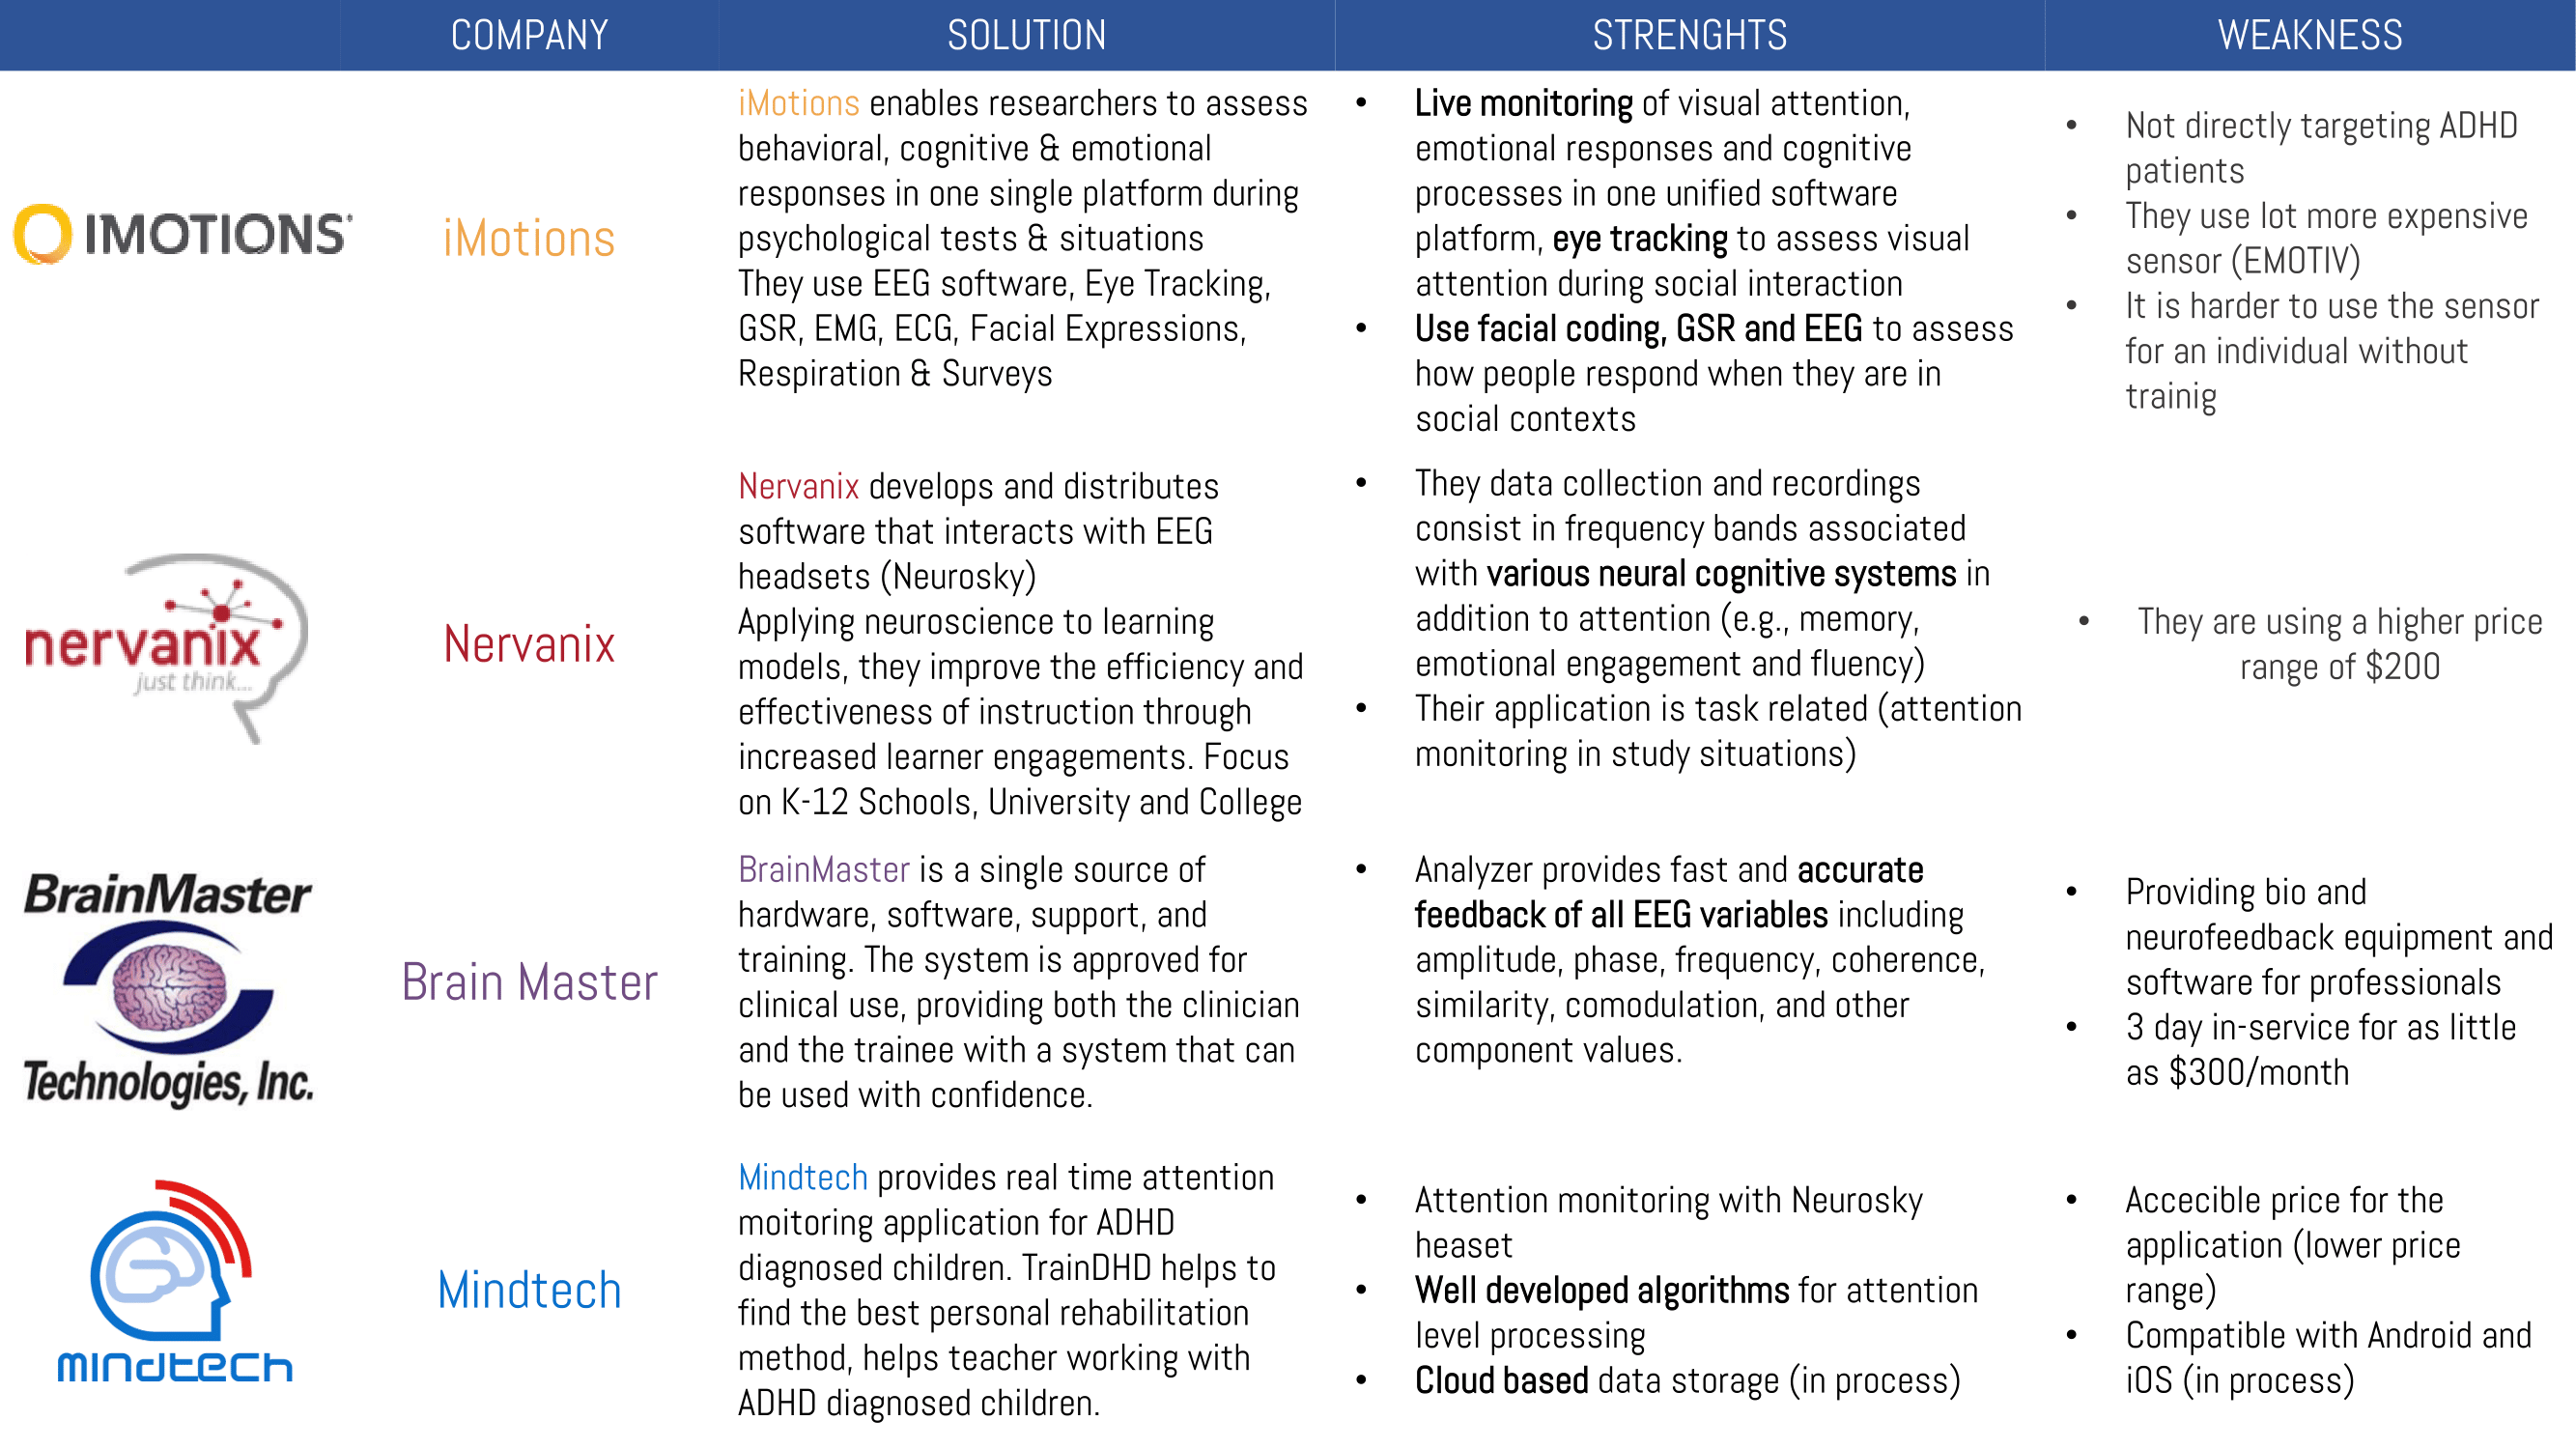
\includegraphics[scale=0.18]{competitive.png}
\captionof{table}{Overview of companies providing service in ADHD solutions}
\label{fig:competiotion}
\end{figure}

\begin{figure}[h]
\centering
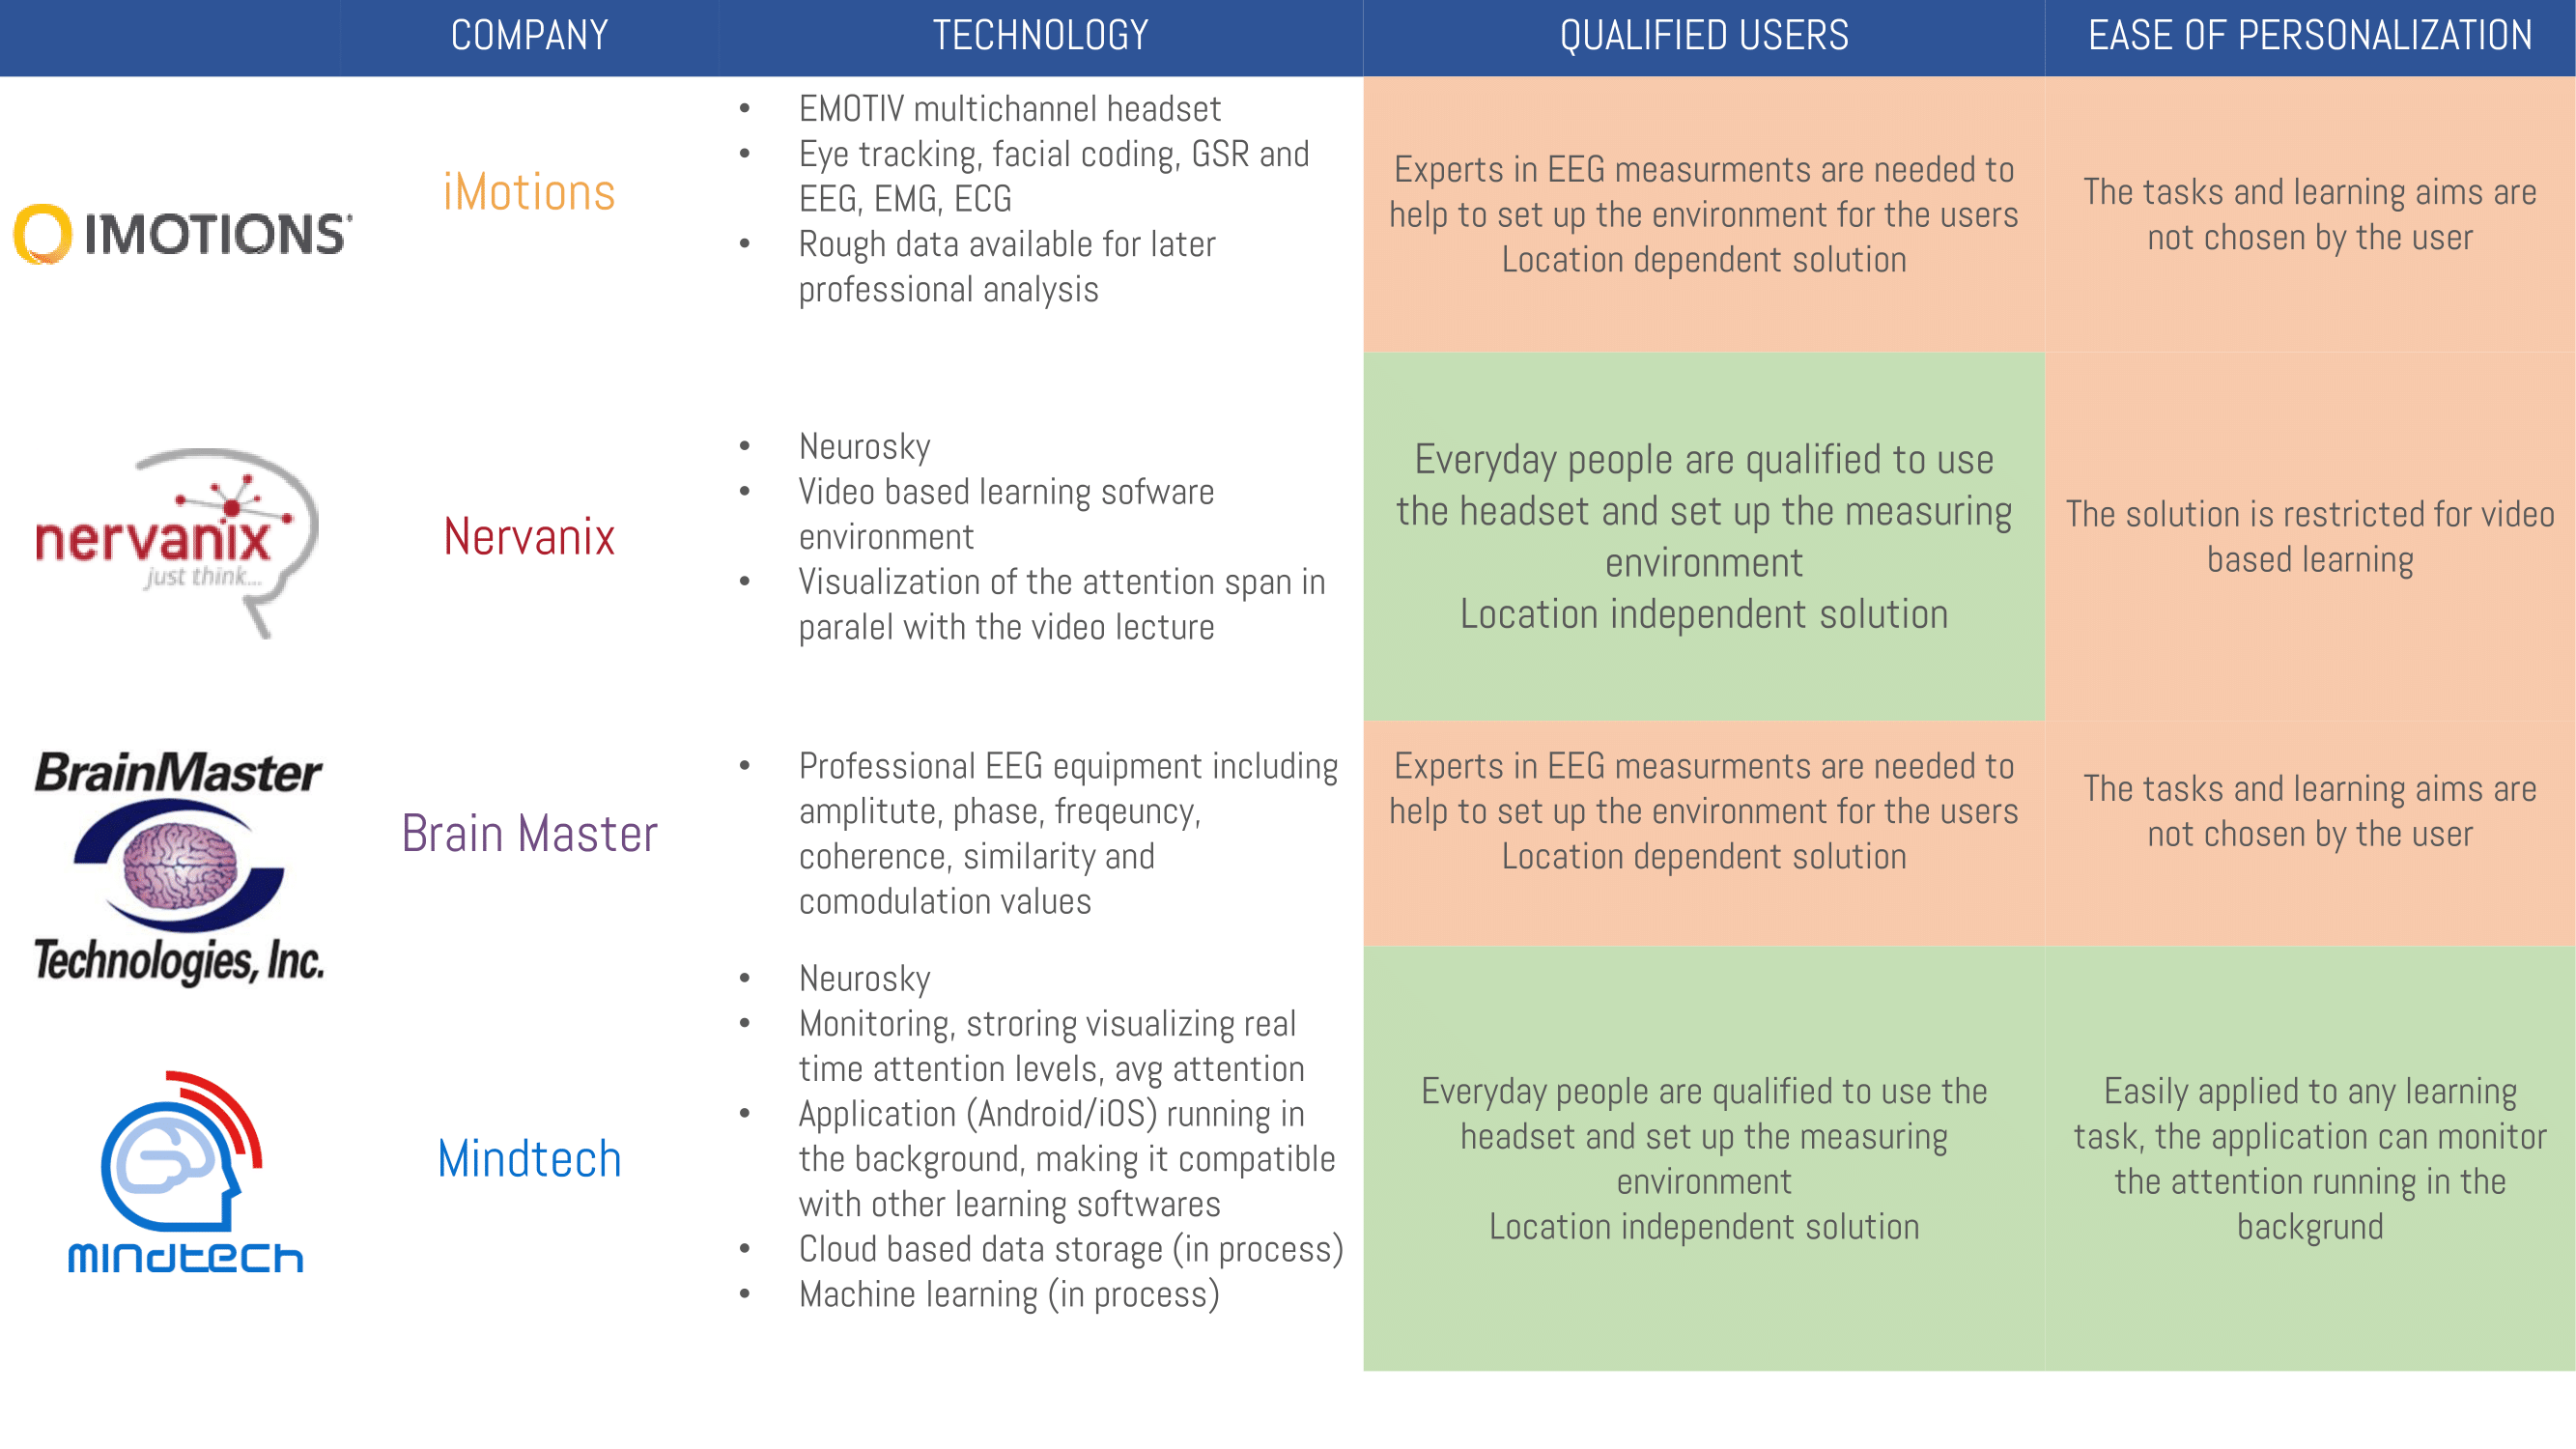
\includegraphics[scale=0.18]{competitive2.png}
\captionof{table}{Competitive advantage of Mindtech's solution among other ADHD neurofeedback solutions}
\label{fig:feature_comp}
\end{figure}

Mindtech finds the best rehabilitation practice for each individual by utilizing real time brainwave data in the most affordable way. Their system consists of a NeuroSky EEG headset and a smartphone with the TrainDHD application. TrainDHD helps trainers find the best rehabilitation practices. Special education trainers perform various training tasks and the software processes the patient's brainwaves and finds the task that caused the highest increase in attention level. It means that TrainDHD helps to find the best personal rehabilitation method. The system helps special education teachers to “take a look” at the paiten"s brain.

During the automated neurofeedback training, patients watch their favorite movies. If they are paying attention, the movie is clearly visible. As soon as the patient is not paying attention, the video starts to fade into black. With the help of Mindtech's system, trainings can be carried out in any environment lowering the stress factor affecting patients.

The data storage of the application is cloud based. Currently the algorithms are based on statistical methods, but we are planning to provide more advanced data analysis using artificial intelligence. \cite{mindtech}

\newpage
\subsection{Conclusion}


Based on the technology review we can say that the market already has a few competitive players with EEG solutions, but Mindtech is the only one providing an easily personable and affordable service to the users. With the possible technology improvements with the cloud-based storage and the machine learning possibilities, Mindtech is able to differentiate itself from the rest of the algorithms providing attention monitoring.


Based on market analysis we can see that there are several possible sub markets to target: children, adolescents and young adults diagnosed with ADHD. In order to find out which of the segments have the biggest need for the solution we can provide, we have to continue our analysis with a detailed customer validation. The next chapter focuses on customer demands and our reshaped value propositions.


\newpage


%%%%%%%%%%%%%%%%%%%%%%%%%%%%%%%%%%%%%% CH 3 %%%%%%%%%%%%%%%%%%%%%%%%%%%%%%%%%%%%%%%%%%

\newpage
\vspace{100mm}
\begin{center}
\uppercase{\Large{Chapter 3}}
\section{\uppercase{\large{Customer validation and business model canvas}}}
\vspace{20mm}
\end{center}


\subsection{Introduction}

In order to propose a strong and viable launch strategy for Mindtech in the U.S. market, every aspect of the business model must be tested and reshaped based on the customers’ needs. The first part of chapter 3 gives a clear insight on the customer segments, the need and pains of the customers within these segments and the value propositions Mindtech can offer to meet these needs.  The second part of chapter 3 concentrates on the key strategies Mindtech must conduct to create a sustainable business. Interviews were conducted to validate or invalidate each hypothesis about the market Mindtech aims to enter.


\subsection{Business Model Canvas}

The Business Model Canvas was created by Alexander Osterwalder, and is a tool that can help both forming or existing businesses easily describe, design, challenge, invent and pivot their business model. This strategic management tool consists of 9 segments, grouped to subsections focusing on customers, value propositions, key infrastructure elements and financial stability. 

\cite{canvas}

\begin{figure}[!htb]
\centering
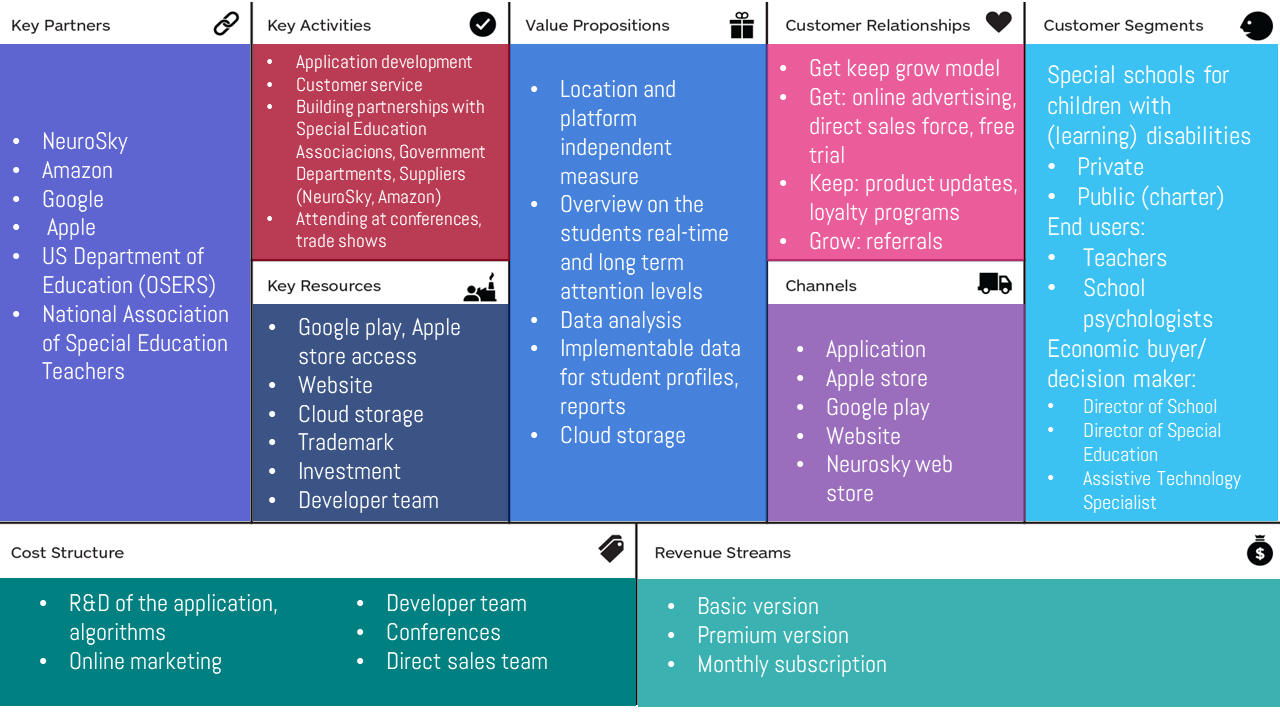
\includegraphics[scale=0.5]{canvas.PNG}
\caption{Business Model Canvas of Mindtech}
\label{img:canvas}
\end{figure}

Figure \ref{img:canvas} presents the Business Model Canvas of Mindtech for the market of ADHD primary inattentive. The canvas is created based on the initial hypothesis on possible markets, interviews from each subsequent will demand changes through the validation process. 


\subsection{Right side of the canvas}

The right side of the canvas focuses on the most important element of the business: the customer. The following sections will present the customer segments and Mindtech's value propositions by using the canvas. Hypotheses for customer relationships, channels and revenue streams will also be stated. 

\subsubsection{Customer Segments}

There are many stakeholders involved in the journey of children and young adults diagnosed with ADHD. Figure \ref{img:adhd:stakeholders} presents the key personas involved with the patients challenges with ADHD. The most closely involved are primary caretakers, friends, the teachers, and school psychologists. Doctors and healthcare are only significantly involved at the diagnosis and medication suggestion stage. Researchers and support groups are continuously involved in the problems. The level of interest and the power to act of these key stakeholders are different. Figure \ref{stakeholders_level_of_int} illustrates that the most interest and power to help the children with ADHD is in the school at which the child is attending. The biggest interests in helping the child although are the parents, primary caretakers, and the private psychologists; however, they do not have enough control and power in most cases.

From the above mentioned stakeholders, the possible customer segments have been selected and categorized further.

\begin{figure}[!htb]
\centering
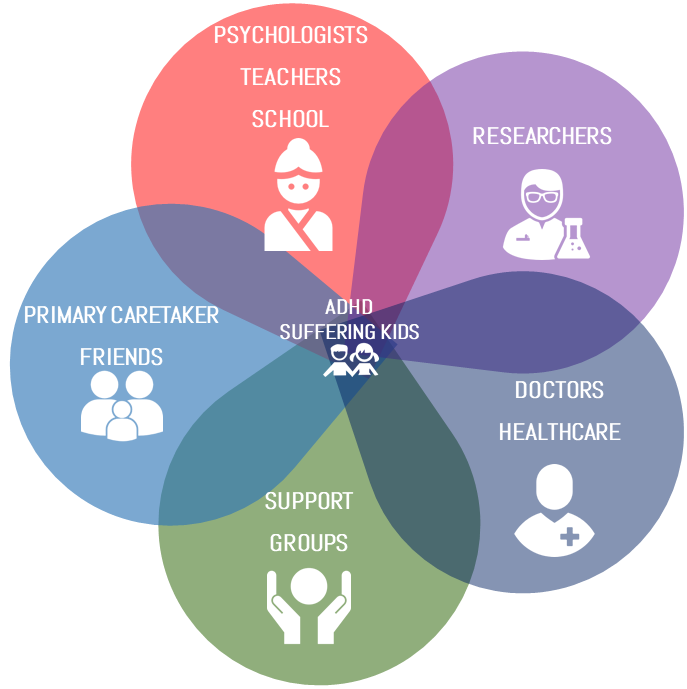
\includegraphics[scale=0.5]{stateholderscircle.png}
\caption{Key stakeholders in the life of children diagnosed with ADHD}
\label{img:adhd:stakeholders}
\end{figure}

\begin{figure}[!htb]
\centering
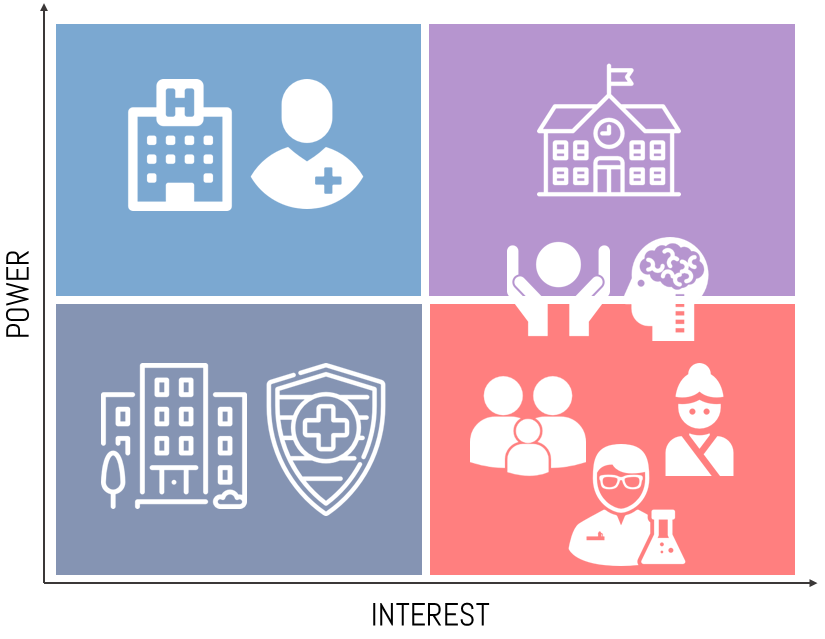
\includegraphics[scale=0.5]{interest.png}
\caption{The matrix of interest and power of the stakeholders in ADHD}
\label{img:stakeholders_level_of_int}
\end{figure}

\begin{figure}[!htb]
\centering
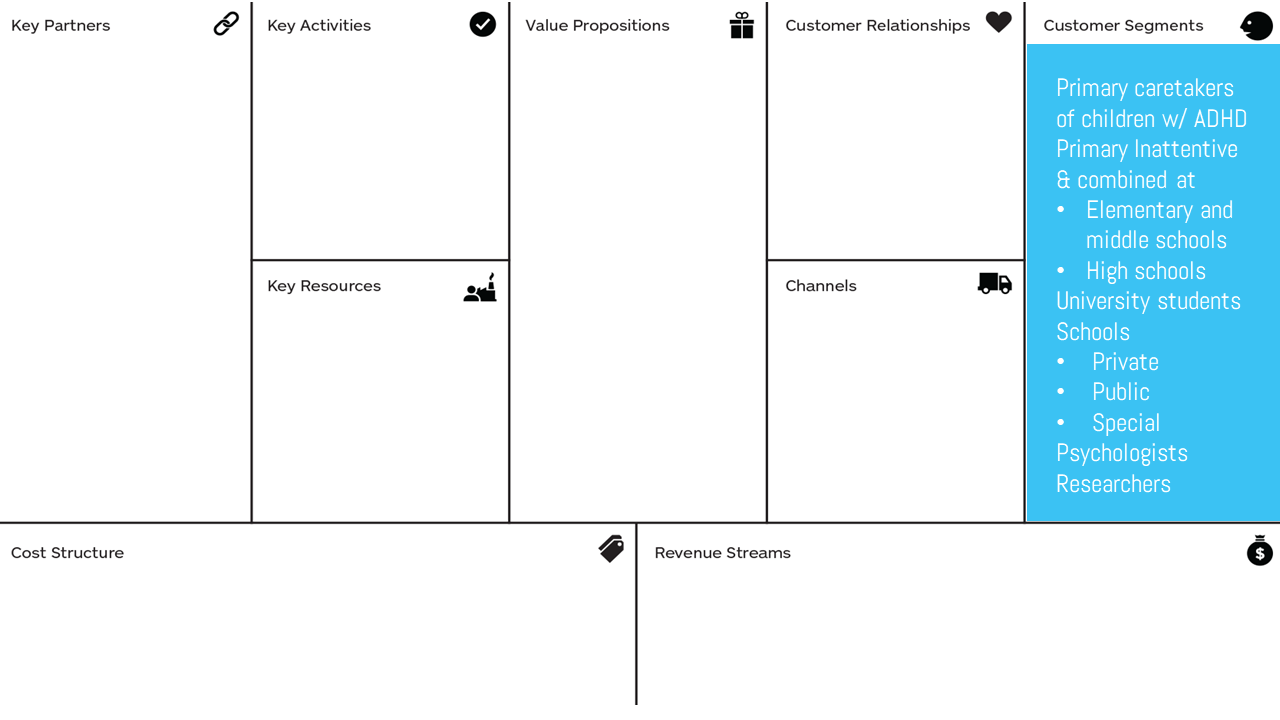
\includegraphics[scale=0.5]{cust.PNG}
\caption{Business Model Canvas - Initial Customer Segments}
\label{img:BMC_cs}
\end{figure}


Figure \ref{img:BMC_cs} shows the hypothesis for the customer segments that Mindtech can serve.

\textbf{Business to customer}

The end users of the software are the children diagnosed with ADHD primary inattentive or combined type, but the analyzer of the brain information in most cases is either the parent, the teacher, the psychologist or the coaches.

The \textit{parents} of ADHD primary inattentive or combined presentation children can be categorized based on their child's age and educational stage. Elementary schoolers, ages 6-12, middle schoolers, ages 12-14, and high schoolers, ages 14-18, attending children's parents or primary caretakers are differentiated. \textit{University students} form a different category, due to their ability to interpret the results of the measurement. Moreover, they are in control of their educational proceedings and are in the decision-making position of purchasing any tool that helps their academic performance. 
\textit{Psychologists} can be categorized into school psychologists, as the end users are part of the business to business (B2B) category, and into private therapists. 


\textbf{Business to business}

\textit{Schools} can be categorized in the same way demonstrated in the previous section: elementary schools, middle schools, high schools and universities all form different subunits. Besides the dropdown based on the stage of education, public, private and special schools, and colleges can be differentiated. 
Special schools or universities are institutions that specialize in working with students with learning differences. A unique subcategory within special schools are college or job preparatory school programs. 
The end user within the schools are the teachers or school psychologists.


\textit{Research institutions} are also a part of the B2B market possibilities, where the researchers designing an experiment about ADHD are our end users. The institutions can be part of University research or individual organizations.


Figure \ref{img:customer_segments} is a visual representation of the customer segments summarized above.

\begin{figure}[!htb]
\centering
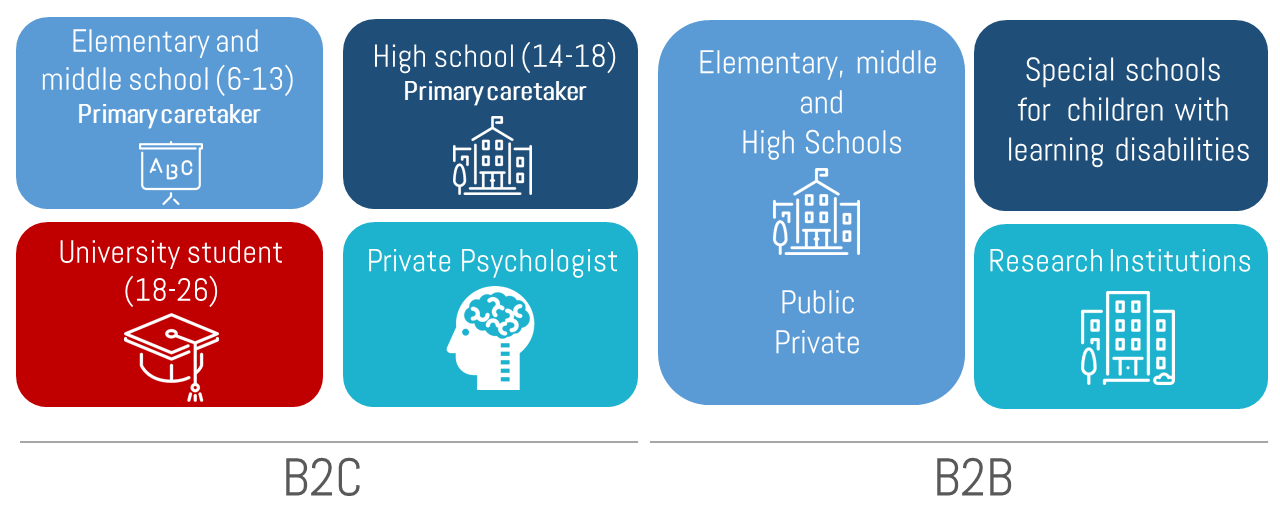
\includegraphics[scale=0.5]{cust_segments.png}
\caption{Mindtech's customer segmentation}
\label{img:customer_segments}
\end{figure}


Mindtech's solution can be targeted to many of these customer segments. At the end of customer validation process, the beachhead market for Mindtech will be clearly defined. 

\subsubsection{Voice of the customer}

In order to map the possible need and the level of involvement of the above-mentioned customer segments, initial interviews with representatives of each segment were conducted. The goal of these interviews was to test the hypothesis of the need for additional support in the journey with children diagnosed with ADHD who have attention problems. 

\paragraph{Interview structure}

In-person interviews are the best way to mark behavioral signs, which either supports or contradicts the information presented. Although each interviewee could not be reached in person, an effort to set up video conferences over phone conversations was made. The initial interview questions were open ended to encourage the interviewee to hit the real pain points and problem generators on his or her own.
Depending on the answers, the necessary questions were always asked to collect the information which help determine the possibilities of Mindtech.

Here are a few examples of typical interview questions. These questions varied based on the persona of the interviewee.

\begin{enumerate}
  \item Can you walk me through the main decision points regarding ADHD diagnosis, and treatment selection?
  \item What are the biggest challenges during ADHD parenting / teaching / therapy?
  \item What are the main problems around the study sessions?
  \item Is there any tool that can help the children focus better?
  \item How does the school provide help for the children?
  \item Are the ADHD resources affordable and accessible location wise?
  \item Is there any technology is already used for attention monitoring/measuring cognitive activity with the children diagnosed with ADHD?
  \item How do you interact with the children diagnosed with ADHD?
\end{enumerate}


\paragraph{Interview insights} \\

\textbf{School psychologists}

From the interviews conducted with school psychologists who were working with kids at K- 12 school settings, or high school, and universities, some important patterns regarding challenges were concluded. Most of the professionals find that the most effective method for treating ADHD is behavioral therapy, although this method needs a strong contribution of parents, teachers and psychologists. Furthermore, this service is not provided in most of the schools. The 1:1 sessions for cognitive training failed to transform into classroom settings, providing long lasting results. There is a large problem with social interaction, and there is no method that can help them better perform with peer interaction. 

Measuring attention levels can be interesting, but feedback will not help the children or parent in terms of a better outcome. 


\textcolor{myblue}{\epigraph{``The teachers and the parents are result orientated. The ultimate goal for therapy is to endorse the children to get their tasks done."; "For middle school and high school kids a tool which would help them with organization, preparation of tasks, studying would be really helpful."}{--- \textup{Dr. George DuPaul},School psychologist, Professor at Lehigh University}}

All in all, based on the recent conversations with school psychologists, they find the best results with behavioral therapy. Until literature shows evidence that supports the better success of neurofeedback, they are not taking the usage of it into consideration. They feel that their patients need better technology assistance with organizing and planning the school responsibilities.


\textbf{Researchers}

From the interviews conducted with researchers, three different point of views on big problems to solve with technology have been concluded. 
In order to improve research tools for understanding the real problems around the behavioral signals, a more evolved technology would be needed, which could detect complex activation patterns. Currently, no imaging or neuroscience tool is capable of such complexity at the level of understanding all mechanisms clearly. Purely attention levels are neither quantitative nor qualitative enough. 

\textcolor{myblue}{\textcolor{myblue}{\epigraph{``EEG activation levels does not necessarily mean that performance is better or worse."; "We don't know what brain activation patterns to look regarding behavior, but it would be revolutionary to measure them."}{--- \textup{Dr. Steven Evans}, Co-Director, Center for Intervention Research in Schools, Ohio University}}}

The problem with the lack of social interaction skills poses a real challenge for patients, and technology could help here with a feedback system on attention at other peer members during teamwork and conversations. 

\textcolor{myblue}{\epigraph{``The neurofeedback training can work if we can apply it to real life situations. I think that in the range of adolescents, an improved neurofeedback training is essential for helping with social interactions."}{--- \textup{Dr. Nora Bunford},ELTE University}}

The main conclusion after each interview was the need for a more accessible solution that can reach every family. Medication has brutal side effects, which make it less desirable to use. 

\textcolor{myblue}{\epigraph{``There is a desperate need for an alternative solution. If a technology could measure cognitive levels within existing tools like smartphones or fit bands, that would be ideal."}{--- \textup{ Dr. Bradley S. Gibson}, ND Psychology Department }}

In conclusion, a need exists for a better, more widely accessible training protocol, but there is not a coherent opinion on what the method should be, and it is clear that attention levels only are not descriptive enough.

\textbf{Parents}

Through the interviews conducted with parents, the biggest weaknesses through the journey of ADHD parenting include: parents are doing their best to provide every resource possible for their children, but in most cases, schools are not supportive enough and private help is expensive. Therefore, medication is the most natural way to help with the problems.

A questionnaire was constructed before reaching out to parents to quantify the problems around the current way of treating children with ADHD primary inattentive and combined presentations. 
139 responses were collected from primary caretakers of children with ADHD. Based on the parents answers besides improper emotional regulations such as meltdowns, stress, and anxiety, 80\% of the children had the biggest problems with schoolwork, homework and focus in the case of the combined and primary inattentive presentations. Parents, on the other hand, are feeling helpless, overloaded with stress, and impatient. Meanwhile, medication is dominating as a resource for the children (86 \%), 50 \% of the responders are providing behavioral therapy and 37 \% of them are paying for private sessions with psychologist. Only 6.5 \% of parents tried neurofeedback with their kids. 
When parents were asked why they were not choosing neurofeedback, they were either unaware of the option, or they were not convinced by the current scientific support on it. Almost half of the responders found the current resources unaffordable at some level, and approximately the same percentage of the responders stated that schools are not providing enough resources for their children. Figure \ref{img:survey} shows the summary of the results, presented above.


\begin{figure}[!htb]
\centering
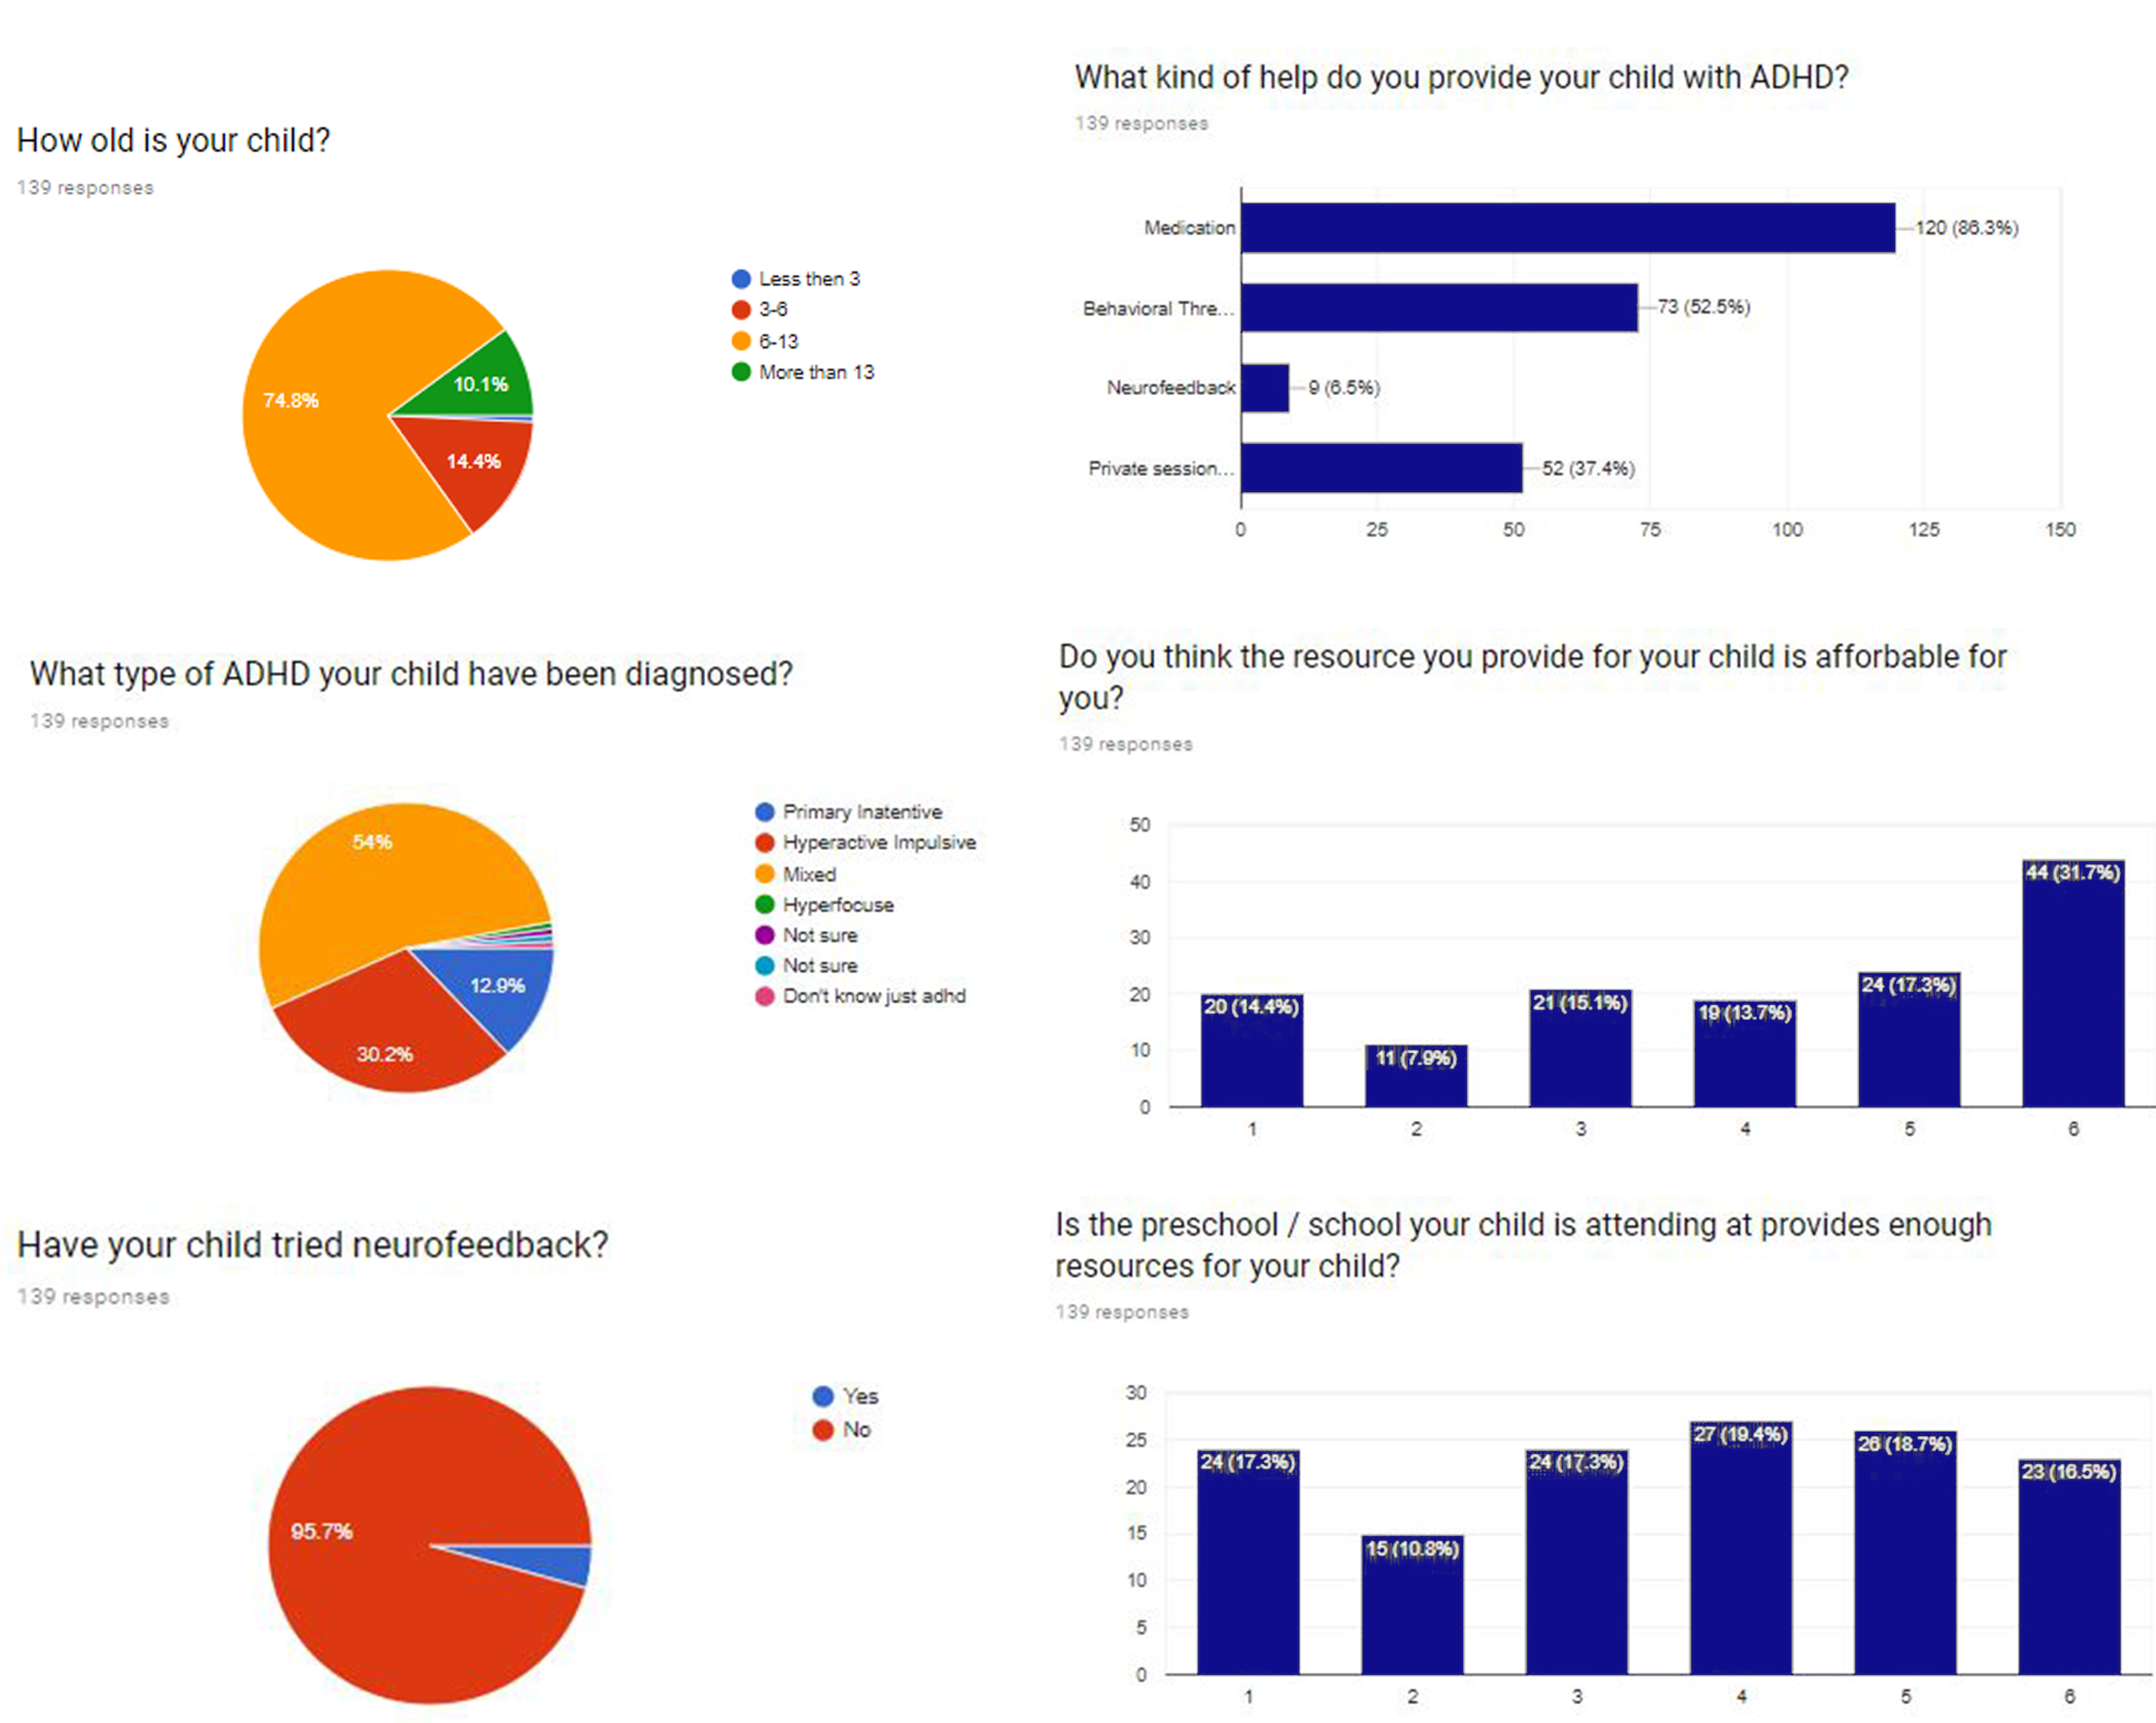
\includegraphics[scale=0.5]{survey.png}
\caption{Summary of survey responses of parents with children diagnosed with ADHD}
\label{img:survey}
\end{figure}


In the value proposition section, the outcomes of detailed interviews targeted to these pain points will be presented.


\textbf{Teachers}

Based on interviews with teachers, a better overview has been gained on the main problems occurring in classroom settings. In public schools, big classrooms are making it nearly impossible for teachers to pay special attention to children with learning disabilities. Although the prevalence of ADHD in a classroom is getting bigger and bigger, with 2-3 cases on average, most public schools have a small and strict budget for special resources. Schools are trying to provide special seatings, including brain break activities during class.

\textcolor{myblue}{\epigraph{``Even if the teacher knows that the child is not paying attention in the class, there is no time for a special intervention."}{--- \textup{Dr. Wendy Folk}, Principal Public Elementary and Secondary Schools in South Bend, 10 years of teaching experience }}

\textbf{University students}

Through interviews with university students, a better solution than medication is needed. Medications not only have very harsh side effects that makes the students case worse sometimes such as heart problems, insomnia, and eating problems, but it is very conditional to get access to it. This leads to cases where students are taking medication only when necessary, and struggling with their study time in between. 


\textcolor{myblue}{\epigraph{``I spend too much time on certain tasks, reading takes me 3 times longer than for others."; "Sometimes I get hyper focused, and get things done a lot faster than others, but other times I am struggling with my deadlines."}{--- \textup{Melissa Holmes}, ADHD primary inattentive, senior Psychology major}}


\subsubsection{Pivots and plans moving forward}

Based on the feedback from possible customers It was possible to conclude that there is definitely a need for an additional solution for ADHD in the following segments: parents, university students, special schools or private schools teachers or psychologists. Although the need for a technological solution varies in every segment, some of the needs cannot be fulfilled with the current state of art regarding BCI solutions. The spectrum of study endorsing technologies is very broad, not everyone is specifically interested in the cognitive levels, most of the parents would be keen on to see specific advice related to behavioral patterns. Public schools neither have the money or ability for special attention to children with learning disabilities, or already have behavioral therapy in action, which apparently excludes neurofeedback. Researchers are looking for more advance technology and protocols, than measuring attention spans. 

In conclusion, a pivot was necessary to identify the ideal beach head market for Mindtech. The focus from just ADHD segment was broadened to other diseases as well, resulting in potential learning problems.

\textbf{Special schools for children with disabilities} \\

\begin{figure}[!htb]
\centering
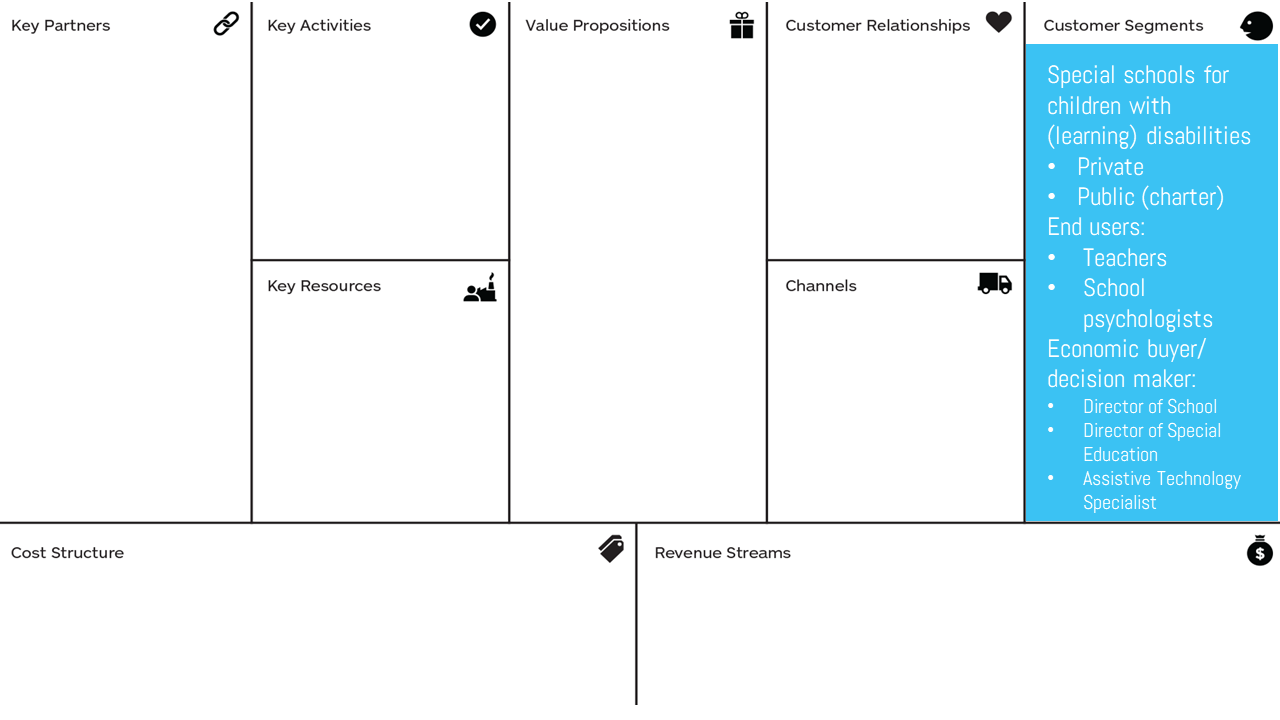
\includegraphics[scale=0.5]{custnew.PNG}
\caption{Business Model Canvas - New customer segment}
\label{img:BMC_newcs}
\end{figure}


The new segment I choose to validate is representing the field of special education. On Figure \ref{img:BMC_newcs} we can see the  I conducted initial interviews with directors of special education institutions. The goal of the interviews was to get a better understanding on the possible needs, pain point of the teachers, heads of the schools when it comes to provide the best learning practices for a child with any kind of learning disability. Here is a list of typical interview questions:

\begin{enumerate}
  \item Can you please indicate the main differences between a public school and the institution you represent?
  \item How you interact with children?
  \item What is the biggest challenge with the education of children with special needs?
  \item How do you measure academic improvement of a student?
  \item How do you measure the level of engagement / improvement when it comes to a non speaking student?
  \item Would attention measure technology help the teachers getting a better feedback on the efficiency on their work? If so, in what way?
\end{enumerate}


\begin{figure}[!htb]
\centering
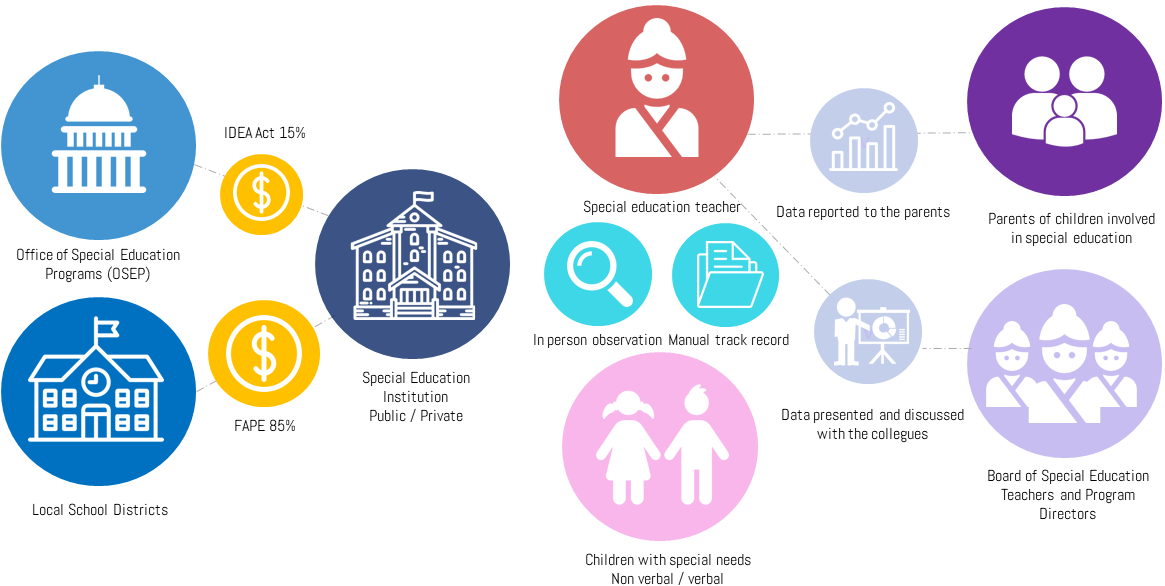
\includegraphics[scale=0.5]{stakeholders_spec.png}
\caption[Stakeholders in Special Education]{Stakeholders in Special Education - Both the Office of Special Education Programs and Local School Districts are funding the Special Education Institutions Operation costs; Teachers are observing the behavior of the children performing a continuous observation, recorded manually; This data on the performance of the children will be monthly reported to parents and discussed with the board of other teachers and institution directors}
\label{img:stake_special}
\end{figure}


On Figure \ref{img:stake_special} the stakeholders in the field of special education are presented. The operation of Special Education Schools are being funded by both government agencies and local school districts. Surprisingly, the considerable amount is provided by the school districts (85\%), under the act of Free Appropriate Education (FAPE). \cite{spec_funding}The Office of Special Education Programs (OSEP) is only supporting up to 15\% through the Individuals with Disabilities Education Act (IDEA). \cite{special_grants} Teachers working with children with special needs usually work in a teacher : student ratio of 3:1. Observing the behavior of the children performing a continuous observation, recorded manually; This data on the performance of the children will be monthly reported to parents and discussed with the board of other teachers and institution directors. A need for a technology that can save time and energy trough the  behavioral management process. 


Base on the takeaways from the initial interviews, it is possible to conclude, that there is a clear need for a technology support when it comes to interact with students who are not able to speak, for example in severe cases of Autism spectrum disorder. Moreover, these institutions are always aiming to decide on the individual education practices, based on data collected on the students performance. There is a lot of observation involved, looking for specific behavioral signals, or educational improvement. Currently these observations are made by teachers, which demands a lot of time and energy. The additional, or in most cases exchanging technology of attention / engagement measurement has a lot of traction from this segment.

Each student has its own profile, including information about their academic performance. If the data collected from the application can be connected to the student profiles, the institution can report to the parents in a very professional way. The online platform for data access and further processing is also a need for these schools.


\textcolor{myblue}{\epigraph{``It would be fantastic to have this technology. If we could measure the level of engagement during learning, we would be able to shape the curriculum, the time determined for a task, corresponding to the exact need of the student."}{--- \textup{Kristina Blackledge}, Founder and CEO of Breakthrough Academy}}


\textcolor{myblue}{\epigraph{``Teachers are continuously rating the students, based on their engagement levels. This technology would be absolutely amazing to provide an objective measure on engagement."}{--- \textup{Sonia Gonzales}, Founder of AZ Aspire Academy}}

\subsubsection{Value propositions}


\begin{figure}[!htb]
\centering
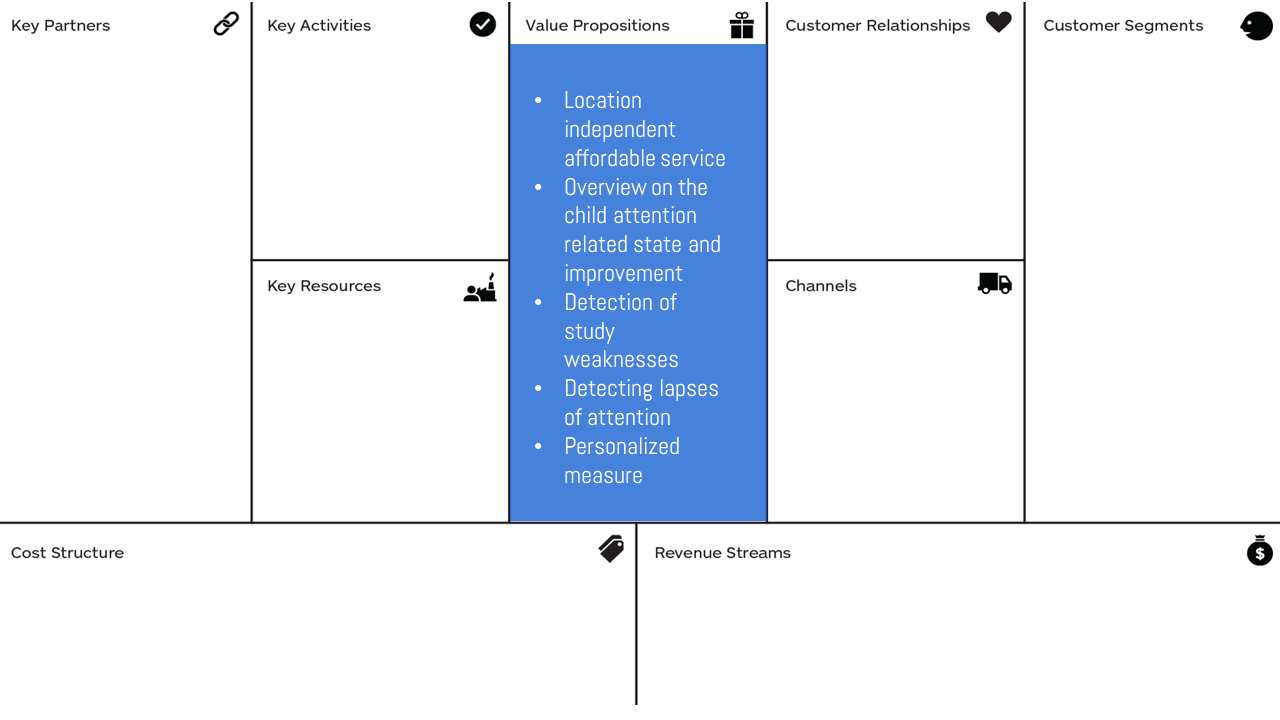
\includegraphics[scale=0.5]{valprop.PNG}
\caption{Business Model Canvas - Initial Value Propositions}
\label{img:BMC_vp}
\end{figure}


Figure \ref{img:BMC_vp} identifies the value propositions and updated customer segments on the canvas. 

\textbf{Parents}

With the help of a tool called value proposition canvas, it is possible the visualize the possible ways of how parents can benefit from the proposed solution. The following design tools represent the hypothesis that needs to be tested further during interviews.


\begin{figure}[!htb]
\centering
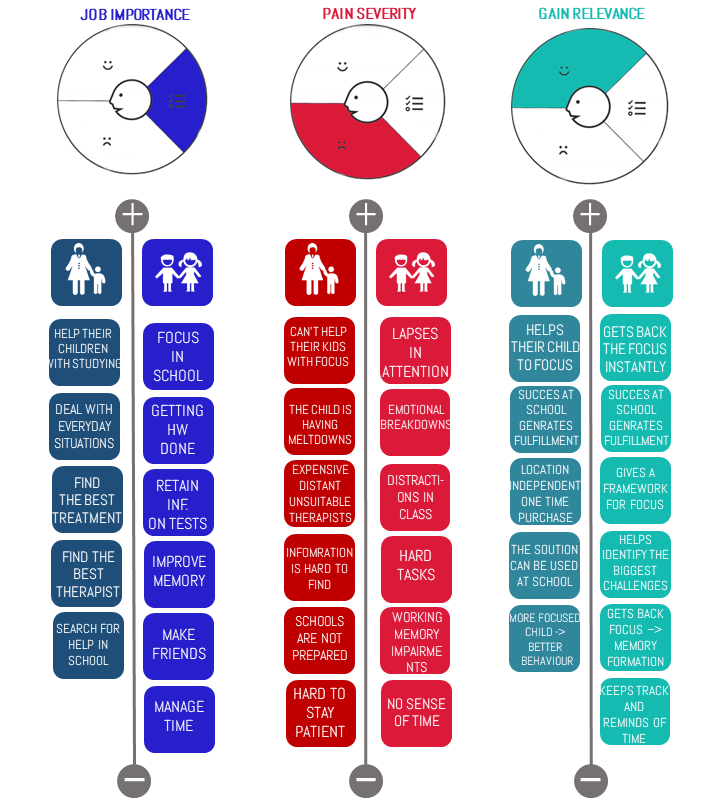
\includegraphics[scale=0.5]{customer_profile.PNG}
\caption{Customer profile of parent and children}
\label{img:customer_profile}
\end{figure}

Figure \ref{img:customer_profile} presents the initial hypothesis on the customer profile. This design thinking tool identifies the jobs, pains and gains of children with ADHD and their parents.  

\begin{figure}[!htb]
\centering
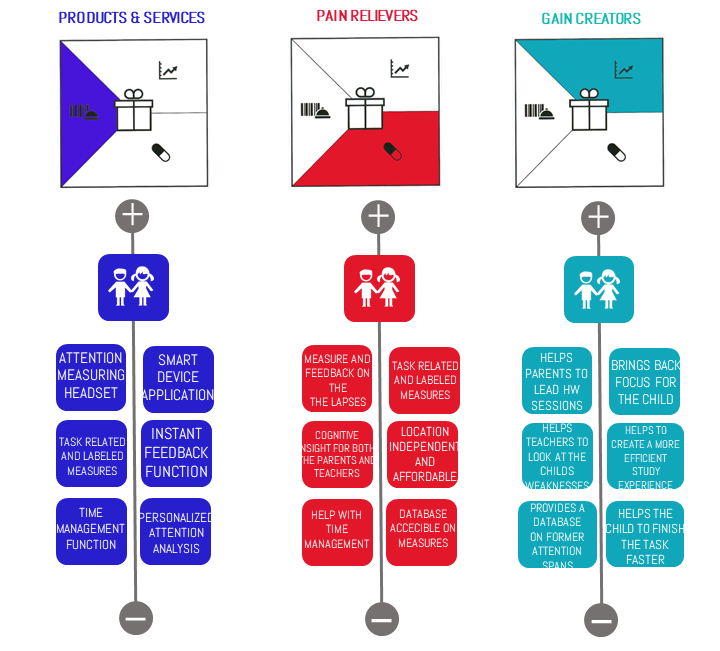
\includegraphics[scale=0.5]{value_map.PNG}
\caption{Value map for children with ADHD}
\label{img:value_map}
\end{figure}


On Figure \ref{img:value_map} the value map about Mindtech's products and services is shown, and the pain relievers and the gain creators are illustrated.   

\begin{figure}[!htb]
\centering
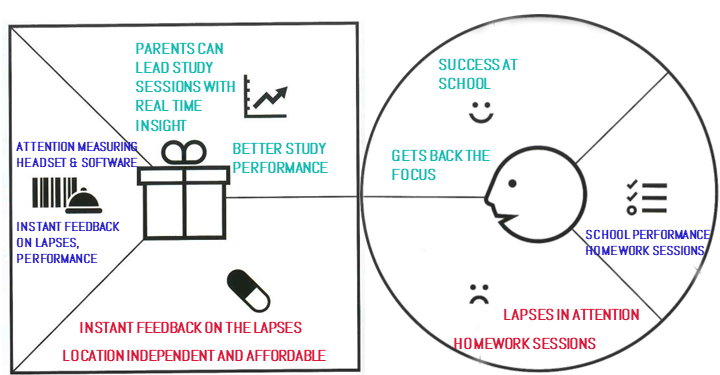
\includegraphics[scale=0.5]{fit.PNG}
\caption{Possible product market fit for Mindtech}
\label{img:prod_market_fit}
\end{figure}

Figure \ref{img:prod_market_fit} represents the proposed product market fit, if the hypothesis is true about the customers’ pains and gains.


\paragraph{Interview insights}

Through six in-person interviews with parents, the following patterns were presented: When it comes to studying, if the children has to deal with a dry or monotonous tasks, or one at the incorrect level of difficulty , the child's attention quickly changes to something else. This does not mean that the child is not paying attention; rather,  he or she gets distracted. The only way to avoid this effect is with very well-developed study material that keeps the children involved and continuously engaged in the task at hand. Unfortunately, teachers are rarely helpful with this process; parents are the ones sitting down with the children and working through the problems with them. If the child has a great protocol for studying with cards, mind-mapping, or games, the study experience is more efficient. 
There are problems when the child is a perfectionist in that he or she keeps challenging him or herself for a better outcome, but never meets the deadline. The biggest challenge is the ability to determine when the inattentive periods are going to come because there are times when the child gets hyper focused, and is able to get tasks done extremely fast.
Based on these parents’ answers, the hypothesis of providing a cognitive tool for parents is getting more and more invaliding evidence.


\textcolor{myblue}{\epigraph{``Looking at brainwaves can be interesting; if the application could tell me what to do when a certain pattern comes up..."}{--- \textup{Elisabeth Ridenour}, Mother of a 3rd grade boy with ADHD primary inattentive}}

\textcolor{myblue}{\epigraph{``My child won’t focus on something boring or monotone. Having the cognitive feedback by itself is not enough for a parent to have better guidance."}{--- \textup{Rachel Kitchen-Cole}, Mother of 2 ADHD primary inattentive children, diagnosed herself as well}}

\textcolor{myblue}{\epigraph{``My children would benefit from something that can help her scheduling better, reminding her of her deadlines."}{--- \textup{Karen Barkely}, Mother of 2 ADHD primary inattentive children}}


\textbf{Special school for ADHD students - Teachers}

Special schools for children with learning disabilities are working with ideal student-to-teacher ratios of 3:1 or10:6. Each child gets special attention in his or her classes, and if it is a boarding school, additional mentors are provided as well. In this setting, the learning material is completely adjusted to the need of the individuals.

The hypothesis to test is whether Mindtech can provide the value of the additional personalized monitoring, weak point detection about the success of the classes, or the study sessions for these high-level institutions. 

\paragraph{Interview insights}

After seven interviews with teachers from special school or preparatory program teachers, the following patterns were observed: Due to small class sizes, the teachers are well aware of the children's performance. Every class activity involves interaction from the students, and if something is not clear for the child, he or she is in a safe environment to ask for help from the teacher and from his or her peers. Additional measurement on attention levels are only interesting when the student comes to the school and he or she has to go through a psychoeducational evaluation with the school neurologist and psychiatrist. 

\textcolor{myblue}{\epigraph{``The students individual needs are met in our institution, we know about their performance without any cognitive testing"}{--- \textup{Kathryn Briggs},The Vanguard School}}


Lendmark college was really interested in the cognitive measure option, but is has its own research lab wherein an eye tracker system is already in place, and possibly new biosensors are also in plan to be set up.

Forman Collage Preparatory School was also interested in the solution, but the fact the students have to wear the headset for proper measurement, it became clear that "labeling" a child with a sensor is not a viable option.


\textcolor{myblue}{\epigraph{``It could be really helpful for the student profiles to see information about attention, but the students won't wear this headset."}{--- \textup{Michael Kowalchick}, Forman Collage Preparatory School}}

\textbf{University students}

The hypothesis in case of university students is the need for an effective tool that can bring their focus back during long study sessions. 

\paragraph{Interview insights}

Through the interviews, a common need was clear among university students with ADHD primary inattentive or combined presentation. The biggest pain points involved scheduling, preparing for deadlines, and getting proper reminders of things that requires the students to pay attention. The ideal solution for them would be a very efficient academic planner that can synchronize information about ideal preparation time for tests, deadlines, and things to remember in one place. An additional cognitive measure could be a “nice to have”, but it is not something that would change the actual material. An additional problem is losing a lot of important items like credit cards, phone, or car keys.

\textcolor{myblue}{\epigraph{``Something that would automatically synchronize the deadlines, action items, and daily tasks from the email/ online materials, would be incredibly helpful."}{--- \textup{Thor Nagel}, Notre Dame student with ADHD primary inattentive presentation}}


\subsubsection{Pivots and plans moving forward}

Based on these initial interviews, the product market fit has not been found yet. There is a clear need for technology solutions for helping students better organizing, remembering their deadlines, and managing their time better. At this point, there is a need for exploring a new market on other learning disabilities, where verbal feedback is not possible from children with these disabilities. Possible developmental disorders to explore include: Autism spectrum, Rett syndrome, and Asperger’s syndrome.

\textbf{Special schools for children with disabilities}

\begin{figure}[!htb]
\centering
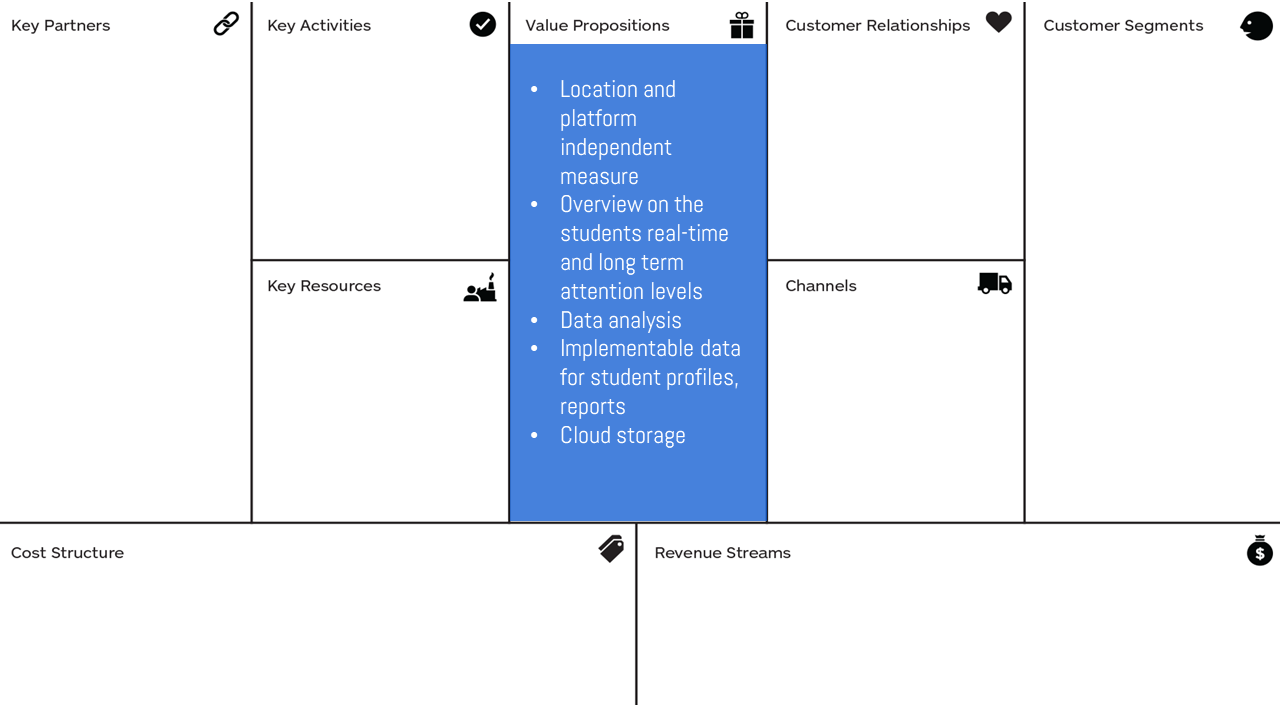
\includegraphics[scale=0.5]{valuenew.PNG}
\caption{Business Model Canvas - New Value Propositions}
\label{img:BMC_newvp}
\end{figure}


As represented on Figure \ref{img:BMC_newvp} as well, Mindtech can provide the following values to the schools working with children with disabilities. A location and platform independent measurement tool, to provide an overview on the students real-time and long term attention levels. For later review, the possibility of data access and analysis is provided, by using a cloud data storage technology. The data is implementable data for student profiles, reports.
In order to validate the need for these solutions provided by Mindtech, a question for the representatives of special schools for children with disabilities was raised about the exact functions they would like to see in an attention monitoring application. 

Mindtech's value proposition consists of the folowing building blocks: 
\begin{itemize}
    \item Saving time for teachers by providing scientific measure on the windows of engagement with the children with special needs
    \item Giving an objective and instant feedback on cognitive information about engagement behind specific behaviors
    \item Providing data management and visualization for trackable results
\end{itemize}

Mindtech's application is a location and platform independent attention monitor tool, for getting insight on the students (especially in the case of a nonverbal student) engagement level through a class activity. 

The web platform connected to the measurement application,  empowers the teachers to access and analyze the data later on, for both increasing the quality of education, and to give a more detailed report for parents. 


\paragraph{Interview insights}

Through the validation process, the need for an easily accessible data storage emerged, among the tools for visualizing the data in different kinds of charts. On the measurement side, the possibility to label the data for later revision, was equally important for every stakeholder. Based on the interviews it can be concluded that the main pain point in special education are around the job of understanding the  In a special education classroom, there is a lot of observation involved, looking for specific behavioral signals or educational improvement. Currently, these observations are made by teachers, which demands a lot of time and energy. The additional, or in most cases exchanging technology of attention/ engagement measurement has a lot of traction from this segment. 

Each student has its own profile, including information about his or her academic performance. If the data collected from the application can be connected to the student profiles, the institution can provide a very professional report to the parents. The online platform for data access and further processing is also a need for these schools.


\textcolor{myblue}{\epigraph{``It would be really interesting to see the patterns of improvement in the student profiles, supported by charts."}{--- \textup{Travis Harris},  Director of Education at Gompers Private School}}

\textcolor{myblue}{\epigraph{``Being able to find the optimal times of engagement with a student would help a lot."}{--- \textup{Courtney Bitting},  Teacher, Imagine Academy for Autism}}


Mindtech's value proposition consists of the following building blocks: saving time for teachers by providing scientific measure on the windows of engagement with the children with special needs, giving an objective and instant feedback on cognitive information about engagement behind specific behaviors, and providing data management and visualization for trackable results.

\begin{figure}[!htb]
\centering
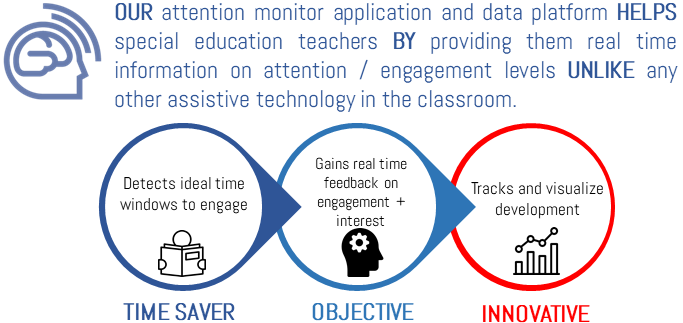
\includegraphics[scale=0.5]{valueprop.PNG}
\caption{\label{img:valprop}Mindtech's value propositions}
\end{figure}

On Figure \ref{img:valprop}, the main value propositions are  visualized. Mindtech's application is a location and platform-independent attention monitor tool for getting insight on the students’ engagement level through a class activity, especially in the case of nonverbal students. The web platform connected to the measurement application empowers the teachers to access and analyze the data later on, for both increasing the quality of education, and to give a more detailed report for parents. 




\subsubsection{Channels}

\begin{figure}[!htb]
\centering
\includegraphics[scale=0.5]{channel.PNG}
\caption{Business Model Canvas - Channels}
\label{img:BMC_channels}
\end{figure}


On Figure \ref{img:BMC_channels} the possible channels Mindtech can use to interact with customers in the learning disability segments: teachers and special institutions is illustrated. Interviews supported the hypothesis of teachers being open to try out new assisting technology applications, these applications are mainly accessible on the iOS App and Google Play store. Mindtech must be present on both platforms to get a great positioning among other applications, show credibility and credentials trough the review system, although because of the great margin these channels take from the applications price - 30 \% - Mindtech will publish only the free version of the software, including an in app purchase function for the full service. On the Mindtech website, the software for Android devices will be available for purchase directly from Mindtech. The iOS software's are mainly restricted to the App store, the direct option is not possible in this case. Kiran Buch, the head of Marketing at NeuroSky confirmed that direct promotion from the NeuroSky website will be provided for Mindtech. 
Mindtech's channel to get in touch with potential customers consists of four elements: the paid online advertisement through Google Adwords, email lists and advertisements on the ABA and NASET website; the direct sales force cold calling and promoting in person for larger deals, attending conferences and trade shows; free and viral social media campaigns; and word of mouth and referrals by current customers. 


\subsubsection{Customer Relationships}

\begin{figure}[!htb]
\centering
\includegraphics[scale=0.5]{rel.PNG}
\caption{Business Model Canvas - Customer relationships}
\label{img:BMC_custrel}
\end{figure}


\textbf{Get} Customers will come in through various levels of advertising, discussed in detail under channel economics. The main channel to which the customers can be informed about the service and request a trial or purchase the subscription is the website, where case studies, testimonials, product reviews, and campaign videos are also accessible. There is a one-month free trial in order to endorse the customers for quicker decision making. 

\textbf{Keep} Mindtech’s existing customers receive engineering support and customer service. The quality of these two services are crucial of keeping the schools on board. The user feedback must be continuously measured and online seminars, monthly emails, and competitions will be created in order to build a community. Loyalty programs will be provided for the automatic subscription extension.

\textbf{Grow} The application will have continuous upgrades with new features to which the customer can upgrade. Teachers who are using the software can become advocates to get other schools on board, in this way getting discounts or unlocking new features. 

Figure \ref{img:gkg} summarizes the get, keep, grow model of Mindtech. The interviews supported that the target segment is likely to try out new products for free trial versions before a purchase, online advertisement on relevant platforms like the ABA website are effective, just like 1:1 sales interactions. Companies providing other SaaS products for the same target segment are mostly using direct sales power as well for a more personal connection, a more effective demo of the technology.


\begin{figure}[!htb]
\centering
\includegraphics[scale=0.5]{gkg.PNG}
\caption{Mindtech's get, keep, grow model}
\label{img:gkg}
\end{figure}

\subsubsection{Revenue streams}

\begin{figure}[!htb]
\centering
\includegraphics[scale=0.5]{rev.PNG}
\caption{Business Model Canvas - Revenue streams}
\label{img:BMC_revstream}
\end{figure}

The interviews conducted with special education teachers showed the that the value of an attention monitoring application would be \$ 10 per student per month for the institutions. If Mindtech combines the attention monitoring service with a more complex system, collecting other ABA related data, the value of the service would increase to \$ 40 per student per month.

Based on the records of the Autism Society, it costs more than \$8,600 extra per year to educate a student with autism. \cite{autism_society} Public special education schools are dominantly receiving funding from Local School Districts, the amount of funding changes in each state, as well as the allocation of funding to assisting technologies. 




On Figure \ref{img:BMC_revstream} we can see the hypothesis for revenue streams for Mindtech. The primary revenue stream comes from special education schools in a B2B model. The schools subscribe for Mindtech’s service for yearly terms, paying subscription fees per student headcount. Figure \ref{img:coststructure} illustrates the building blocks of Mindtech's cost structure. For the basic product, which consists of the attention measurement application and the data processing platform, the student subscription fee per month is \$10 for larger schools, and \$15 for smaller schools. The combined product, containing the ABA measurement functions, has a price of \$35 and \$40, respectively. This price contains the troubleshooting services, full customer support and implementation. For every new customer there is a free monthly trial period provided.

\begin{figure}[!htb]
\centering
\includegraphics[scale=0.7]{coststructure.PNG}
\caption{Mindtech's pricing strategy}
\label{img:coststructure}
\end{figure}

\subsection{Left side of the canvas}

\subsubsection{Key activities}

\begin{figure}[!htb]
\centering
\includegraphics[scale=0.5]{activ.PNG}
\caption{Business Model Canvas - Key activities}
\label{img:BMC_keyact}
\end{figure}


On Figure \ref{img:BMC_keyact} we can see the list of the key activities Mindtech have to perform. Before the launch of the product the development of additional features, incorporation of beta testing feedback is necessary. Establishing strong partnerships with the US Special Education department and NeuroSky is also important for a strong start. Attending at assisting technology conferences, trade shows can speed up customer validation, bring the early adopters on board. Providing a professional customer service and troubleshooting is a key for making sure, that the schools on board are satisfied with Mindtech's service.                                                                                        


\subsubsection{Key partners}

\begin{figure}[!htb]
\centering
\includegraphics[scale=0.5]{part.PNG}
\caption{Business Model Canvas - Key partners}
\label{img:BMC_keypart}
\end{figure}


On Figure \ref{img:BMC_keypart} we can see the hypothesis for the key partner Mindtech have to acquire. 

The US Department of Education Office of Special Education Programs (OSEP) provides grants to assist the 50 states special education schools. These funds are allocated among states in accordance with a variety of factors, indicated under the Individuals with Disabilities Education Act (IDEA). Each state has the liberty of allocating the funds for different purposes, including the category of improving the use of technology in the classroom and technical assistance. \cite{grants} 
Mindtech's innovation can fit in to both of these subgroups. There are several grants endorsing the development of technology support for the special and public education classrooms. Based on the interviews conducted with both the National Initiatives and Elemtary and Middle School subdivision of OSEP, Mindtech fits into this category and has a strong enough model to be considered for support. Previous cases studies are necessary to build a strong argument for Mindtech's impact on the empowerement of teachers.


Mindtech must build strong partnership with NeuroSky to overcome the challenges around headset dependence. The support of NeuroSky can provide beneficial offers for schools on headsets purchases, and a strong credibility in the field of educational technology. Furthermore, a partnership with the Office of Special Education Programs is necessary for gaining the trust of the schools and the promotion of the government. Moreover, the partnership with fundraisers and endowments is necessary for creating successful campaigns.


\subsubsection{Key resources}

\begin{figure}[!htb]
\centering
\includegraphics[scale=0.5]{res.PNG}
\caption{Business Model Canvas - Key resources}
\label{img:BMC_resources}
\end{figure}


On Figure \ref{img:BMC_resources} we can see the hypothesis for the key resources Mindtech have to acquire. Mindtech needs to acquire a website domain focusing on the special education services, a cloud storage plan, ideally with Firebase and a Google Play and Apple store profile for the free trial services. A strong developer team and early investors are essential for the fast market entrance.


\subsubsection{Cost structure}

\begin{figure}[!htb]
\centering
\includegraphics[scale=0.5]{cost.PNG}
\caption{Business Model Canvas -Cost structure }
\label{img:BMC_coststruct}
\end{figure}


On Figure \ref{img:BMC_coststruct} we can see the hypothesis for the cost structure Mindtech have to create. Mindtech have to put a big emphasis on Research and Development to create the most competitive software, including each round of early adopter testing. The customer satisfaction is extremely important, the first users of the software become the advocates for Mindtech's technology. Online marketing and a direct 1:1 sales team is also essential for the early success, based on the interviews the importance of in person sales, conference attendance, and the main web channels used has been identified.





\subsection{Conclusion}

This chapter gave the overview on the Business Model Canvas, with big emphasis on the voice of the customer. After a major pivot on the served marked, from students diagnosed with ADHD to students suffering from Autism spectrum disorder, Rett syndrome or Down syndrome, Mindtech identified a large beachhead market in form of special education schools. The main pain points of the lack of feedback on engagement were presented, among other possible applications. In the next chapter the intellectual property landscape and the competitive analysis of Mindtech will be discussed.


\newpage
\newpage
\newpage

%%%%%%%%%%%%%%%%%%%%%%%%%%%%%%%%%%%%%% CH 4 %%%%%%%%%%%%%%%%%%%%%%%%%%%%%%%%%%%%%%%%%%

\newpage
\vspace{600mm}
\begin{center}
\uppercase{\Large{Chapter 4}}
\section{\uppercase{\large{Intellectual property and competitive analysis}}} 
\vspace{20mm}
\end{center}

\subsection{Introduction}

Before Mindtech enters the market of technology solutions for learning disabilities, it is important to focus on intellectual property (IP) protection, and the creation of a stable legal environment for both Mindtech’s applications and the company itself. Furthermore, it is essential to analyze the direct and indirect competitors, highlighting the competitive advantages and weaknesses of each.
The goal of this chapter is to present an overview of the intellectual property and legal landscape on Mindtech's solutions, which includes the fundamental laws involved in a technology startup. Moreover, the competitive landscape of Mindtech and its solutions will be presented, among which will be a strengths, weaknesses, opportunities, and threats (SWOT) analysis of both Mindtech and its competitors. 

\subsection{Intellectual Property overview}

The intellectual property overview of software companies is different. In general, they do not protect their products by means of patents, since software has short innovation cycles. Software industry differs from other industries in this regard. Customarily, copyrights and trade secrets provide the necessary protection. This combination can provide adequate incentives, and is flexible enough in this fast changing environment.  \cite{goldman_2012}
 
Copyrights protect the form of expression, meanwhile trade secrets may secure both the concept and manner of expression in case of a software. \cite{patent_book}


\subsection{Patents}

In terms of intellectual property protection, computer software programs can be protected, to a limited extent, by patents, among copyrights and trade secrets. Patents on computer procedures protect the concept or idea behind the software regardless of how it is specified. \cite{goldman_2012}

The process from filling and acquiring a patent is long and circumstantial, yet software solutions tend to be iterated quickly. The application and features of software usually have an effective commercial life of a few years. After new software developments, these versions quickly override the prior obsolete innovations. 

Mindtech's source code is based on NeuroSky's Inc Developer Tools, and therefore is not patentable. This is because it cannot be described as nonobvious or novel. Mindtech does not own the whole solution; NeuroSky provides a part source code for the application whereby the software receives the raw and processed EEG data from a NeuroSky Mindwave mobile headset. 

However, it is important to make sure that Mindtech or NeuroSky is not infringing with other patents regarding EEG signal processing. 

NeuroSky has patented the way of measuring brainwaves by the electrode it uses in its headsets. Moreover, NeuroSky has pending patent applications for the methods of bio signal processing when it comes to mobile applications. 

\begin{table}[htb!]
\centering
\caption{Patent applications of NeuroSky Inc}
\label{patents_NeuroSky}
\begin{tabular}{|l|l|l|l|L|}
\hline
\multicolumn{1}{|c|}{\textbf{No.}} & \multicolumn{1}{c|}{\textbf{Type}} & \multicolumn{1}{c|}{\textbf{Date}} & \multicolumn{1}{c|}{\textbf{Application \#}} & \multicolumn{1}{c|}{\textbf{Title}}                    \\ \hline
1.                                 & Granted - US                            & 1/14                               & 20130211226                                  & Dry electrode device and method of assembly.           \\ \hline
2.                                 & Application - US                       & 7/14                               & 20140210709                                  & Bio signal based mobile device applications.           \\ \hline
3.                                 & Application - US                       & 9/13                               & 20130237867                                  & Modular user-exchangeable accessory for bio-signal controlled mechanism. \\ \hline
\end{tabular}
\end{table}

In table \ref{patents_NeuroSky} the list of the NeuroSky patent relevant to Mindtech's project is illustrated. 

One possible risk here could be the lack of either a patent application or a granted patent on the algorithm, which is performed through the RAW EEG signal processing, or a patent on the TGAM chip, which performs the calculations.
It is necessary to ensure that NeuroSky's technology is not infringing with other patents related to the fields mentioned above. 

\begin{table}[htb!]
\centering
\caption{Result of patent search on EEG processing algorithms and units}
\label{patent_search}
\begin{tabular}{|l|l|l|l|L|}
\hline
\multicolumn{1}{|c|}{\textbf{No.}} & \multicolumn{1}{c|}{\textbf{Type}} & \multicolumn{1}{c|}{\textbf{Date}} & \multicolumn{1}{c|}{\textbf{Application \#}} & \multicolumn{1}{c|}{\textbf{Title}}                                                             \\ \hline
1.                                 & Granted - US                       & 11/17                              & 20150313496                                  & Mobile Wearable Electromagnetic Brain Activity Monitor.                                         \\ \hline
2.                                 & Granted - US                       & 2/16                               & 20130179087                                  & Methods and Systems for Determining, Monitoring, and Analyzing Personalized Response Variables Using Brain Wave Frequency Data and Interactive Multimedia Display. \\ \hline
3.                                 & Granted - Korea                    & 5/15                               & 101517007                                    & BCI input interface system and method for serious game.                                                                    \\ \hline
4.                                 & Granted - China                    & 10/14                              & 203898306                                    & Brain wave collecting device based on wireless transmission.                                                          \\ \hline
5.                                 & Granted - China                    & 11/12                              & 202537499                                    & Head brain wave detector.                                                                       \\ \hline
\end{tabular}
\end{table}

Table \ref{patent_search} summarizes the results of a patent search on the possible EEG processing algorithms and units. After examining the claims in these results, it is concluded that patents granted in Korea and China could be a source of danger for Mindtech to bring a solution to the market. If these patents had filed in the US, further examination would be necessary. Therefore, the patents granted in the US are not a possible source of infringement that either Mindtech or NeuroSky could commit. 

\subsection{Legal relationship with NeuroSky}
NeuroSky product families consist of hardware and software components for simple integration of this biosensor technology into consumer and industrial end-applications.
Since a part of Mindtech's technology is based on NeuroSky solutions, by developing solutions for the NeuroSky Mindwave Mobile headset, Mindtech must agree to NeuroSky's License Agreement. NeuroSky is providing developers the ability to use the developer tools in order to create applications after agreeing to the Developer Agreement document. NeuroSky also states publishing requirements and application standards.

\subsubsection{NeuroSky License Agreement}

The License Agreement for using NeuroSky’s devices and software contains important restrictions of which Mindtech must be aware. Mindtech has to respect that all \textit{"NeuroSky Algorithms, Hardware, Software, and Guide and any accompanying or related documentation, including technical data, delivered as related to this Agreement are commercial within the meaning of Federal Acquisition Regulation."}

Furthermore, the License Agreement states that \textit{"nothing herein shall be construed as a right or license to make, have made, use, sell, offer to sell, import, lease or distribute any products or technology related to the Products, the Hardware, the Software or the NeuroSky Algorithms, or to use any name, identifier, trademark, trade name, service mark or other designation of the Company".} This segment could prevent Mindtech from using the base of NeuroSky software as part of its solution. However, NeuroSky endorses developers to create solutions using the hardware and the core software solution. A different agreement regulates the rights of the developers, as discussed in the following section.  \cite{neuro_licence_agreement}

\subsubsection{NeuroSky Developer Agreement}


NeuroSky’s technologies enable and encourage product developers to create solutions that can make an impact in the industry of personalized health. The company provides free resources and detailed guidance for developers to build applications compatible with the NeuroSky Mindwave Mobile headset. The NeuroSky Developer Agreement contains the regulations relevant for developers. NeuroSky differentiates itself by providing building block component solutions that offer friendly synergies with related and complementary technological solutions.

\textit{"The NeuroSky product families and related documentation is provided "as is" without any express or implied warranty of any kind including warranties of merchantability, non-infringement of intellectual property, including patents, copyrights or otherwise, or fitness for any particular purpose. In no event shall NeuroSky or its suppliers be liable for any damages arising out of the use of or inability to use the NeuroSky".} In the Warnings and Disclaimer of Liability section the following is stated: \textit{ "the algorithms must not be used for any illegal use. Your use of the software development kit, the algorithms and any other NeuroSky products or services is “as-is,” and NeuroSky does not make, and hereby disclaims, any and all other express and implied warranties, including, but not limited to, warranties of merchantability or fitness for a particular purpose, and any warranties arising from a course of dealing, usage, or trade practice."} \cite{about_neurosky}

\subsubsection{NeuroSky Publishing Requirements}

NeuroSky has several publishing requirements among other legal constraints. For every developer, it is necessary to provide a brief description of the application including its main features, three to four pictures of the program in action, and an altered version of the icon template to indicate the program inside of the store. \cite{publish}

\subsubsection{NeuroSky Application Standards}

NeuroSky understands the importance of flexibility and freedom at the design of application. It is imperative to set a uniform visual language for any solution connected to the NeuroSky headset. It raises the bar for any applications that it helps to distribute and promote. Third-Party applications like Mindtech fall into the categories of the NeuroSky App Store-promoted solution. \cite{app_standard}


\subsection{Trademark}

Mindtech can have additional protection by acquiring a trademark on the company's name and logo.  Trademarks make different products distinguishable for customers, and a strong mark is usually imaginative, arbitrary, or suggestive. It is important to check in the United States Patent and Trademark Office (USPTO) database to determine if the Mindtech name and logo can be registered. Upon searching USPTO, “Mindtech” does not infringe upon a symbol or name used by another company operating in the same market.  
According to the USPTO, there is one live trademark with the name Mindtech registered with the serial number of 86773074 and submitted on September 15th, 2017, and describes a children's educational software. This product is a virtual reality software for classroom education. The owner of the trademark is TutorTech Group LLC, located in Nashville. 
Mindtech is offering a software solution as well, therefore applying for a trademark need a very well stated application, enhancing the main differences: Mindtech is the name of the company, not the name of the product; and Mindtech is providing a BCI solution in the market of learning disabilities. 

For the name “trainDHD”, there were no results in the USPTO database, and therefore presents no barrier for filing a trademark application. \cite{trademark_search}

\begin{figure}[!htb]
\centering
\includegraphics[scale=0.8]{logos.png}
\caption[Mindtech and trainDHD logo]{Mindtech and trainDHD logo to be registered in the United States and Hungary}
\label{img:logo_trademark}
\end{figure}

Figure \ref{img:logo_trademark} shows the logos of both Mindtech and the mobile application trainDHD to be registered in the United States and Hungary as well. The name “Mindtech” reflects the technological aspect of the solution, the idea of utilizing brainwaves to provide innovative solutions. “trainDHD” is a keyword specifically for training children with ADHD.

Unlike patents and copyrights, trademarks do not expire after a given period. Rather, they are active as long as it is being used by the owner. On the tenth anniversary of registration, the owner must prove that the mark is still in use. \cite{about_trademark}

\subsection{Copyrights}

There are multiple aspects of an application that can qualify for copyright protection. These include the source code itself, the object (compiled) code, the visual layout, the documentation, or even the aggregation of menu commands, called user interfaces. In other words, the structure, sequence, and organization of the software can all be protected. \cite{goldman_2012}

The combination of copyright and trade secrets can provide the substantial intellectual property protection for any software.

A copyright is gained automatically at the time the source code, user interface is created. However if Mindtech aims to enforce a copyright against someone making an unauthorized copy, must obtain a certificate of registration of a copyrightable work from the United States Copyright Office. The duration of a copyright can be maximum 70 years from creation. \cite{protect_IP}

It is important to note that each version of a computer program containing new, copyrightable authorship is considered a separate work. The developers must submit a new application, filing fee, and deposit for each version they want to register. \cite{copyright_article}


\subsection{End User License Agreement}

The End-User Licensing Agreement (EULA) is a crucial part of any mobile application. The EULA is a contract between the end user of a mobile app and the software developer. 

The contract works between the user of the mobile app and the provider of the application, or software developer, to distribute a license to the user of the app. Mindtech owns the intellectual property and only a license can be passed on to the user.
The license includes limitations such as prohibiting the user from aiming to reverse-engineer or resell the software.

The agreement includes clauses such as use restrictions, termination of licensing, and disclaimer of liability. The restrictions on the use section forbids the user’s utilization of the application for generating a profit or attempting to decrypt the application. The termination of license segment includes a clause to take away the grant of use in case of a violation of the application. In the disclaimer of liability section, Mindtech's liabilities are discussed, specifically highlighting the consequences of any potential damage raised from the use of the application. \cite{termsfeed_2016}
 
A suggestion for an End User License Agreement for the trainDHD application can be found in Appendix \ref{appendix:eula}.  After the buyer downloads and installs the application from the App store or Google Play store and opens the software for the first time, the EULA must be accepted in order to continue.
 


\subsection{User Terms \& Conditions}

Mindtech's mobile application will use a Terms \& Conditions Agreement along with the EULA document, since it has both a mobile application and an online service component by storing data on a server. Terms and Conditions is a set of rules to which the user must agree in order to use the Mindtech's trainDHD application, and is a legal contract between Mindtech and the user who access the mobile application. \cite{termsfeed_2017}

The User Terms \& Conditions Agreement is segmented into 14 subsections and is as follows: 1. Accounts and Membership 2. Backups 3. Links to Other Mobile Applications 4. Advertisements 5. Prohibited uses 6. Intellectual Property Rights 7. Limitation of Liability 8. Indemnification 9. Severability 10. Warranty and Disclaimer 11. Assignment 12. Dispute Resolution 13. Changes and Amendments 14. Acceptance of Terms. The Intellectual property rights section informs the user about the trademarks registered by Mindtech, including graphics and logos that are protected by trademark laws. Users can create an account in the application, and in the “Accounts and Membership” section, the responsibilities of the user are listed, such as providing valid information and being accountable for any activity under the account. In a free version, Mindtech's application can have advertisements. Thus in the “Advertisements” and “Warranty and Disclaimers” section, Mindtech clarifies that it takes no responsibility or liability for any transaction between the user and any third-party application or product advertised on or through Mindtech’s service. By including the section “Prohibited Users”, Mindtech can maintain rights to exclude users from the application in the event that users abuse the application, uses it for any unlawful purpose, violate any international or federal law.


A possible User Terms \& Conditions document for the trainDHD application can be found in Appendix \ref{appendix:terms}. The user has to agree to these terms after installing the application, among the EULA document. Both agreements will be accessible for the user for later review under the “Legal Agreements” tab. 

\subsection{Mindtech Company Structure}

Mindtech was registered as a Limited Liability Company in Hungary in August of 2015 with the registration number, 13 09 176759. \\
In order to expand Mindtech's market into the United States, it is necessary to register the company in the United States as well. Before choosing a suitable business organization form, it is important to consider the following factors: cost of creating the company, methods of wealth creation, management, limits of personal liability, and taxation laws. 
One the most popular legal entities for a startup is the LLC, because it is easy to register and have ideal taxation advantages.  

A Limited Liability Company (LLC) is a business form that is a separate legal entity for liability purposes, but not for tax purposes. An LLC has more than one member who pays income tax as a partnership, and the individual members pay taxes based their share in the ownership; there is no double taxation, as federal taxes are not involved. The management is flexible, there are no strict book requirements, and a board of directors is not necessary. Changes can be made easily in the case of an LLC; new partners can be added, or the interest can be sold to new members. Each owner’s personal assets are protected in the case of an LLC, although the possibilities are limited for later acquisitions and merges after the company has expanded. \cite{boitnott}





\subsection{Competitive analysis introduction}

The market of different ADHD related solutions is significantly increasing each year, as more and more patients are being diagnosed. As indicated in Chapter 1, three different categories of solutions are differentiated: medication comprising of stimulants and non-stimulants, behavioral therapy which necessitates the strong contribution of psychologists, parents and teachers for the result of a positive behavioral change in the children, and neurofeedback, a training method using real time attention levels for acquiring better cognitive skills.
Mindtech falls under the third category due to the inclusion of a real-time attention measurement as well as a feedback and sensitive monitor system around it. There are many technological solutions either within or strongly related to neurofeedback, and the following sections present the analysis of these competitive solutions on the market.





\subsection{Competitive landscape}

The competitive landscape of technological solutions for ADHD primary inattentive presentation has many players, as many of these approaches consist of biosensors, smart device application development, or well developed neurofeedback systems. The previous chapter presented the technological components of neurofeedback systems: the sensors and the different software's measuring and processing the real-time attention level of the patient.
Not every possible competitor utilizes biosensors to measure the cognitive skill development of the user. Some of them solely rely on well-developed training programs to increase attention, working memory, and analytic skills.
The following subsection will present the companies that provide solutions for children, adolescents, and young adults diagnosed with ADHD primary inattentive representation with the purpose of increasing different cognitive skills including attention, working memory, and focus.

\subsubsection{Competitor profiles}

To categorize the company profiles mentioned above, both a horizontal and a vertical measure is presented. EEG sensor free and EEG sensor related solutions will be differentiated, as well as mixed cognitive improvement involving attention, working memory, analytic skills, and attention focused applications. In figure \ref{img:comp_map}, Mindtech's competitors are positioned examining these factors. 

Looking at the possible features of cognitive training solutions or attention measure options, we can conclude that by the solutions nature – EEG sensor based and attention focus solution – Mindtech has Nervanix as the biggest competitor. But if we are looking at pricing and location independence, on Figure \ref{img:comp_pos}, we can see that Nervanix is not low cost or flexible enough with location (providing a PC based solution rather than a hand device software). The biggest competitors with price and smart device solutions are brain training games, not providing scientifically proven cognitive measures, and their efficiency is not well proven. The white space for Mindtech is clear: low cost & location independent (smart divide application with portable sensor) solution.


\begin{figure}[hbt!]
\centering
\includegraphics[scale=0.5]{map_comp.png}
\caption{Competitors profile matrix of Mindtech}
\label{img:comp_map}
\end{figure}

\begin{figure}[hbt!]
\centering
\includegraphics[scale=0.7]{comp_pos.png}
\caption{Competitors positioning matrix of Mindtech}
\label{img:comp_pos}
\end{figure}

\subsubsection{Traditional neurofeedback}


Traditional neurofeedback sessions are location-dependent services with multichannel EEG sensors. The biofeedback software is specified for the direct training of the brain functions, creating a visualization of the different cognitive levels. The patient’s task is to consciously modify levels which include: decreased muscle tension, increased alpha levels, and decreased beta levels. The system rewards the patient for altering the brain patterns to more appropriate levels.

Table \ref{img:neurofeedback_tabla} summarizes the main profiles of the traditional neurofeedback companies.

\begin{figure}[h]
\centering
\includegraphics[scale=0.5]{neurofeedback_comp.PNG}
\captionof{table}{Competitive analysis of traditional neurofeedback companies}
\label{img:neurofeedback_tabla}
\end{figure}

\newpage

\paragraph{Neurocore}

\begin{comment}
\begin{figure}[h]
\includegraphics[scale=0.5]{Neurocore-Social-Share.png}
\label{img:neurocorelogo}
\end{figure}
\end{comment}

Neurocore is private held company founded in 2012, situated in Cleveland. They have around 75 emloyees and an estimated yearly sales of \$ 109,939. \cite{mergent_intellect}



Neurocore provides data-driven, brain-based diagnostics and treatments that help children and adults improve concentration, sleep and stress management. The company provides neurofeedback therapy to train the brain to operate efficiently through positive feedback and repetition. It offers diagnostics in the areas of ADHD, anxiety, autism, depression, migraines, sleep, and stress. \cite{bloomberg}

Neurocore has brain performance centers in several cities in Michigan, which include West Bloomfield, Grand Rapids, Grandville,  Holland, Livonia, and Sterling Heights, as well as Boca Raton and Palm Beach, Florida. The pricing of the neurofeedback session is \$2,200 /30 sessions. Some insurances cover the amount, the company provides a free consultation about insurance check. 
\cite{neurocore}

Neurocore services are currently in-network with Blue Cross Blue Shield of Michigan and BlueCare Network. The firm is one of 13 businesses that are part of The Windquest Group, the Grand Rapids-based holding group owned by Dick and Betsy DeVos, Educational Secretary.

\cite{neurocore_loc}

\subsubsection{SWOT analysis of Neurocore}

\begin{figure}[h]
\centering
\includegraphics[scale=0.4]{neurocore_swot.PNG}
\caption{SWOT analysis of Neurocore}
\label{img:neurocoreswot}
\end{figure}

Figure \ref{img:neurocoreswot} demonstrates the SWOT analysis of Neurocore.

\paragraph{Strengths}

Neurocore is targeting not just attention problems regarding ADHD primary inattentive , but co-symptoms of anxiety, possible depression, sleep, and stress problems as well. It  has many locations around Michigan, and session costs can be covered by insurance. It provides free assessments and consulting about insurance coverage.

\paragraph{Weaknesses}

It is a location-dependent service without a robust portfolio. The science behind its method of brain training is not yet finalized. It is questionable how effective it methods are. “The scientific community has definitely not reached consensus on the utility of neurofeedback.”

\cite{boser_2017}


\paragraph{Opportunities}

In addition, expanding its current brain training centers to other locations, the company has other big opportunities as well.
Betsy DeVos has invested millions of dollars in Neurocore, and as the Educational Secretary, she has the power to make strong connections with schools and universities to help create on-site training centers. With this opportunity, Neurocore can reach a great deal of clients, making its service more reachable.


\paragraph{Threats}

The company is robust enough to be a target to criticism around its credibility. Several articles can be found online, doubting the honesty of the company: "Neurocore offers false hope to people who need honest help ."
If a strong enough evidence is found that this claim is real, this can destroy the company's profile .


\cite{boser_2017}


\paragraph{iMotions}

\begin{comment}

\begin{figure}[h]
\includegraphics[scale=0.5]{iMotions_logo.png}
\label{img:imotionslogo}
\end{figure}
\end{comment}

iMotions is a private company founded in 2005 and is based in New York. With an estimated 11-50 employees, it is still considered as an early stage startup. They have yearly sales approximately of \$1,000,000. \cite{mergent_intellect}

iMotions’ software platform is developed to synchronize, visualize, and analyze cognitive research with eye tracking, facial expression analysis, galvanic skin response, surveys, and EEG . Additionally, it is providing assessments for cognitive and emotional responses.

\cite{pitchbook}

Researchers can assess, predict, and treat cognitive health-related problems such as ADHD, autism, OCD, and depression with the help of the iMotion platform. Above ADHD symptoms of inattention like attention, memory, and perception, they can help with stress, anxiety, sensation, sleep, and biorhythms motor control . They provide cognitive, behavior social and developmental aspects of training. Researchers are also selling software and hardware elements including EEG monitoring devices, eye trackers, and other biometric signal measuring tools.
iMotions’ pricing is not available for the public, and the customer has to request a pricing for the specific solution or hardware component they wish to explore. iMotions has offices in Boston and Coppenhagen. 

\cite{imotions}

\paragraph{BrainMasters}

\begin{comment}
\begin{figure}[h]
\includegraphics[scale=0.5]{brainmasterslogo.png}
\label{img:brainmasterslogo}
\end{figure}
\end{comment}

BrainMasters is a privately held company founded in 2008 and based in Cleveland. It has 5-10 employees, with yearly sales of \$110,000. Its main source of revenue comes from selling quantitative EEG software and neurofeedback devices for clinics and professionals like psychiatrists, and therapists. Its neurofeedback software pricing can vary in the range of \$500-\$900.
The BrainMaster system is approved for clinical use. Leading clinicians, educators, and researchers are using its system. Its mission is to provide the highest quality of clinical training or remote home training, and to make it economically available.

\cite{brainmasterscom}

BrainMaster has an official neurofeedback center called the Brain Enrichment Center and is located in Bedford, Ohio. First, patients complete a computer-based assessment that measures cognitive performance in areas such as memory, reasoning, attention, and processing speed. It identifies specific abnormal brain patterns that relate to symptoms, and creates a personalized training plan to encourage healthier brain function. 
The neurofeedback training utilizes BrainMaster’s technology products, with either a 4-channel measurement, Level 1, or a 19-channel measurement, Level 2. After the sessions are completed, a second quantitative EEG measurement in conducted, and it compares the changes. 

\cite{bmlocation}

The Brain Enrichment Center is part of two professionl affilications: the Association for Applied Psychophysiology and Biofeedback (AAPB) and International Society for Neurofeedback and Research (ISNR).

The cost per session is not shared with the public, as this information is only shared after scheduling a consultation. 

\subsubsection{Sensor free brain training games}



A lot of smart device applications both indirectly and directly target patients with ADHD. These solutions do not require any brain monitoring sensors because both the assessment and improvement track is based on the user’s performance in specific brain games. The algorithms behind these cognitive games have proven to be efficient in estimating the user’s memory, attention, and analytic skills. There are a lot of similar applications available, but only the most highly rated ones are presented here.

On Table \ref{img:braingames_tabla} the company profiles of sensor free brain training games are demonstrated. 

\begin{figure}[!htb]
\centering
\includegraphics[scale=0.5]{braingame_comp.PNG}
\captionof{table}{Competitive analysis of brain game commertializing companies}
\label{img:braingames_tabla}
\end{figure}

\newpage

\paragraph{Cognifit}

\begin{comment}
\begin{figure}[h]
\includegraphics[scale=0.5]{cognifitlogo.png}
\label{img:cognifit_logo}
\end{figure}
\end{comment}

Cognifit is a privately held company founded in 2000 and based in New York city. It has 51-100 employees, and an annual revenue of \$1,100,000. \cite{mergent_intellect}


The Cognifit app is available both in the App store and Google play. The assessments before any training are provide a professional tool to detect cognitive alterations . It tracks the user’s cognitive skill evolution and compares the results to age group norms. The training program consists of personalized brain games, measuring and evaluating focused and dividend attention, visual perception, and visual scanning skills.

The target users are health professionals looking for better diagnoses on cognitive disorders: schools and researchers who would like to track cognitive skills, individuals with concentration problems, memory, focus, mental planning, and depression.

The application itself is free to download, but without purchasing a plan, the content is not accessible. For individuals, the access costs \$20/month; for professionals, the cost is dependent on the number of patients in the system. For example, the annual cost is \$1,380 per 10 patients.

\cite{cognifit}

\subsubsection{SWOT analysis of CogniFit}

\begin{figure}[h]
\centering
\includegraphics[scale=0.4]{cognifit_swot.PNG}
\caption{SWOT analyisis of Cognifit}
\label{img:cognifit_swot}
\end{figure}

Figure \ref{img:cognifit_swot} demonstrates the SWOT analysis of Cognifit.

\paragraph{Strengths}

The Cognifit software provides a great combination of both assessments and training games. It not only serves ADHD diagnosed patients, but users having problems with depression, dyslexia, dyscalculia, insomnia, or Parkinson's disease. The software doesn't require the purchase or use of any EEG-measuring device, which makes it use more convenient. Cognifit is available in many languages with a flexible monthly license option.

\paragraph{Weaknesses}

Unlike other similar software on the market, Cognifit has no free version. The users cannot get a demo on the software, unless he or she signs up for a monthly subscription. This strategy causes Cognifit to lose many potential customers. 

\paragraph{Opportunities}

Cognifit has many opportunities to make strong connections with health professionals who are looking for better diagnoses for cognitive disorders. Schools and researchers who would like to track cognitive skills are a couple examples of beneficiaries of Cognifit.


\paragraph{Threats}

A lot of similar brain game platforms, such as Elevate and Lumosity, are already competing in this market, with free versions of their solution as well. If either enterprise gains a great reputation by participating in a well-founded study, the focus of the users can be moved away from Cognifit.
Just like other brain training game solutions, the threat of inefficiency and bad customer reviews is the biggest challenge Cognifit has to face.

\paragraph{Elevate}

\begin{comment}
\begin{figure}[h]
\includegraphics[scale=0.5]{elevatelogo.png}
\label{img:elevate_logo}
\end{figure}
\end{comment}


Elevate Labs is privately held company with headquarters in San Francisco. The company was founded in 2014 and now has 11-50 employees. Its annual revenue is approximately \$689,236. \cite{mergent_intellect}

\cite{mergent_intellect}

The Elevate application debuted in 2014, and was rated the best iPhone application of the year. It provided a personalized brain training program that adjusts over time based on performance. It focuses on attention, memory, processing speed, and comprehension training.


Elevate designed more than 40 games to boost productivity, earning power, and self-confidence in skills like math, reading, writing, speaking, and listening. It introduced a special scale factor called the Elevate Proficiency Quotient (EPQ). The EPQ measures the user’s performance in the subsections . Based on the user’s performance, the EPQ can range from 0 to 5000, and can go up or down compared to previous performances.


The application enables three free games daily. The premium membershipm which costs \$5/month or \$45/year, provides unlimited access to the games.

\cite{elevateapp}

\paragraph{Lumosity}

\begin{comment}
\begin{figure}[h]
\includegraphics[scale=0.5]{lumositylogo.png}
\label{img:lumosity_logo}
\end{figure}
\end{comment}



Lumos Labs is a privately held company founded in 2006 with headquarters in San Francisco. It has between 100-150 employees with an annual revenue around \$6,247,798. \cite{mergent_intellect}

\cite{mergent_intellect}

The Lumosity app is one of the biggest competition of Elevate, providing personalized cognitive games designed to improve memory, focus, and problem solving skills. The application detects the baseline of the user by a three-game assessment, then generates daily workouts for the five core cognitive abilities. The games always adapt to the users skill level. Additionally, Lumosity tracks the user’s personal improvement. 

Lumos Labs collaborates with more than 100 researchers worldwide, providing them free access to their brain training tools. 

The free version of Lumosity provides three free games daily. The premium membership with unlimited access costs \$15/month or \$80/year.

\cite{lumosity}

\subsubsection{Sensor related brain training applications}

The direct competitors of Mindtech are software solutions that use real-time brain data from location-independent EEG measuring tools. This type of software can be either neurofeedback solutions or attention level monitor solutions related to a study setting. No company developing smart device applications have been found in a preliminary search; the solutions are usually software for personal computers and laptops.

\begin{figure}[!htb]
\centering
\includegraphics[scale=0.5]{sensor_comp.PNG}
\captionof{table}{Competitive analysis of sensor related brain training application providing companies}
\label{img:sensorapps_tabla}
\end{figure}

\newpage

Table \ref{img:sensorapps_tabla} summarizes the competitive analysis of the sensor related brain training application providing companies.

\paragraph{Nervanix}

\begin{comment}
\begin{figure}[h]
\includegraphics[scale=0.5]{nervanixlogo.png}
\label{img:nervanix_logo}
\end{figure}
\end{comment}


Nervanix is a privately held company founded in 2016. It is 11-20 employees, and an estimated annual revenue of \$1,000,000. 

\cite{mergent_intellect}

Nervanix is also operating in the educational technology sector, as its solution is the closest to Mindtech's, using the same headset and a similar algorithm. The goal with their computer softwares is to improve attention and focus in order to optimize student engagement and achievement. 

It measures attention levels of learners, both in real time as well as longitudinally, and uses that information to enable learners to self-monitor their studying and learning.
The solution is useful for teachers as well, as they are able to see the efficiency of their teaching methods. Nervanix solution is targeted for learning platforms as well, with a purpose to align and match appropriate learning objects to individual learners based on attention profiles.
 
\textbf{Insight}

The Nervanix Insight application provides real-time feedback on the user’s attention levels, which is measured through the Mindwave mobile headset.
 
This software allows access to an online learning library. Through the study session, when the user’s EEG activity proves a focused, attentive state, the screen brightens and remains bright. If the attention level drifts, the screen starts to fade away. To read the material clear again, the attention level must increase. After the end of each study session, a report is made showing the chart of attention related to time.

\textbf{Clarity}


Nervanix Clarity measures attention levels of learners as they study, and follows the user’s attention along as he or she navigates a page, watches a video, listens to a recording, or interacts with digital content.

This software allows the user to pin information along the way to identify the areas of high and low attention. If the user revises these pin points, he or she can better understand, with the help of attention span, which parts were highly interesting, confusing, vague, or anything in between.
 
Nervanix Clarity provides users with the possibility to review specific sections of material multiple times until they are satisfied with their attention levels and overall study session.

\textit{Insight} or \textit{Clarity} comes in a package with a headset for \$200 with a one-year license. For the professional version, used for practitioners, the cost of the software is \$100 / session.


\cite{nervanix}


\subsubsection{SWOT analysis of Nervanix}

\begin{figure}[!htb]
\centering
\includegraphics[scale=0.4]{nervanix_swot.PNG}
\caption{SWOT analysis of Nervanix}
\label{img:nervanix_swot}
\end{figure}

Figure \ref{img:nervanix_swot} demonstrates the SWOT analysis of Nervanix.


\paragraph{Strengths}

One of the biggest strengths of Nervanix is the ability to reach to more customer segments with two software solutions. It targets corporate learning centers, learning centers , schools and colleges and students learning at home. The software solutions are well-built around online study materials; the feature of marking segments of the study session for later revising is advanced. The company  

\paragraph{Weaknesses}

The educational material compatible with the software is limited to video files, Khan Academy tutorials, and Youtube videos. The current version of the product is not compatible with PDF, .doc or .ppt formats. This restriction makes the software less flexible for any study setting. Its pricing is license-based annually. This setting is also very strict for flexible learners.

\paragraph{Opportunities}

Nervanix already made connections with K-12 schools, a case study is available about a contribution with Calcasieu Parish School District. They have a lot of opportunities to expanding their client list to Universities and Colleges, smaller Companies.

\paragraph{Threats}

Nervanix has other competitors out there with similar solutions; it is exposed to new software developed for the NeuroSky headset. The headset manufacturer can alter the price of the device and the regulations around the software development for the NeuroSky Mindwave Mobile as well.

\paragraph{Play Attention}

\begin{comment}
\begin{figure}[h]
\includegraphics[scale=0.5]{playattention.JPG}
\label{img:playattention_logo}
\end{figure}
\end{comment}


Play Attention is a privately held company, found in 2012 and based in Cleveland, Ohio. It has 10-15 employeeswith annual sales of \$109,939.

Play Attention provides a learning system to improve attention, behavior, and cognitive function for ADHD children and adults. Play Attention’s software is based on neurofeedback technology. The user can control the computer, or move game characters, by attention alone. 
Unlike clinical EEG, Play Attention uses a non-clinical brain energy monitor housed in an armband called BodyWave. BodyWave monitors brain signal indicative of attention and cognitive processing. 
 
The company is not transparent with pricing, but indicates that the home user format costs less than \$5 a day. The client has to sign up to find out the exact cost of the hardware and the license.

\cite{play_attention}

\paragraph{Brain Train}

\begin{comment}
\begin{figure}[h]
\includegraphics[scale=0.5]{braintrain_logo.JPG}
\label{img:braintrain_logo}
\end{figure}
\end{comment}


BrainTrain is a privately held company founded in 2008 and headquartered  in Cleveland, Ohio. It has 15-20 employees with estimated annual sales of \$110,000. 

\cite{mergent_intellect}

BrainTrain develops professional cognitive training software and EEG biofeedback systems called neurofeedback. These products are designed to help people ages 13 and above the abilities to learn to think, focus, read, and remember.

The cognitive software, in the form of games, trains users’ working and short-term memory as well as attention, processing speed, impulse control, listening, and problem-solving skills.
It provides solutions for both licensed practitioners, via the Smart Mind 3 neurofeedback, and for everyday users as well, via Attention Gym.

\textbf{SmartMind 3} 

This software may be used only under the supervision of a licensed practitioner for the purpose of relaxation training. It is equipped with a cloud-based technology, enabling the practitioner to work at an independent location. The software  trains the executive functioning center of the brain by using games to exercise attention and relaxation.

The access of the software for one year for 1 user costs \$395; for 5 users, \$995. A five-year license including other training software as well costs \$5,495. 

\textbf{Attention Gym}


The BrainTrain Attention Gym is designed to help users improve their attention to detail as well as listening and concentration skills. 

The Attention Gym features a reward system consisting of seven different types of game breaks. During the brain training games, the user can monitor his or her own state of concentration, using the optional BrainPower system, which requires a MindWave headset. The BrainPower system helps foster a positive, alert, relaxed, and focused mental state.

The pricing of the software varies based on the number of users and the length of access.  
One year with unlimited players costs \$995 and one year with one player costs \$149.
 
Brain Train is also sells NeuroSky MindWave Mobile headsets for a price of \$149. The same headset ordered from the manufacturer costs \$100.

\cite{braintrain}

 
\subsection{SWOT analysis of Mindtech}

\begin{figure}[!htb]
\centering
\includegraphics[scale=0.4]{swotketto.png}
\caption{SWOT analyisis of Mindtech}
\label{img:mindtechswoti}
\end{figure}


Figure \ref{img:mindtechswoti} illustrates the SWOT analysis of Mindtech.

\subsubsection{Strengths}

Mindtech's product focuses clearly on the users attention related performance, provides a real time attention measure overview on a session for in time intervention or later review. The service is platform independent, any smart phone or tablet can be used for the measure, unlike other similar realizations, running only at PC-s. The end user has the flexibility of performing the measures anywhere, not interrupting any classroom activity, not altering the results with the pressure of a strict measuring environment. The recorded brain data is stored in the cloud, teachers, administration or parents can get access to the results. The online platform has endless possibilities, the dat  There are several additional measures applicable, tracking the personal improvement of the student, visualizing the data in requested ways. 

After necessary amount of data has been collected, a learning dataset will be provided for further analysis. With the amount of information collected, there are very promising machine learning possibilities, for more personalized cognitive measures, algorithms can be implemented for a better data analysis for the end user. Mindtech's team is very flexible when it comes to development, the software is at early phase, user feedback can be easily implemented.

\subsubsection{Weaknesses}

Mindtech's biggest weakness is the lack of tests and data collection about the possible user case. The lack customer user base leads to the lack of testimonials, which could give credibility for other users about the products efficiency. Research and development is still in process, an in the world of applications, fast publishing is essential. Moreover, the necessary purchase of the NeuroSky headset can slow down the implementation process.
A weakness is coming from the fact, that the solution is not patentable, only copyrights and trade secrets are protecting the solution. 
Furthermore, Nervanix has a very similar profile to Mindtech, providing a similar solution as a computer software. Mindtech needs to differentiate itself with a more clear value proposition and use case scenario. 

Mindtech also needs to find a way to partner with distributors, find a channel which has a more reasonable margin than the 30\% Google play or App store. 

\subsubsection{Opportunities}

Mindtech has wide opportunities in the area of special education for children with learning disabilities. Beside the schools working with students with neurodevelopmental disorders, such as ADHD, Autism spectrum, Rett syndrome, and Asperger’s syndrome, Dyslexia, the market can be expanded to parents having nonverbal children.
Before even the product shows a great demand, it is a big opportunity for Mindtech to get promoted in the NeuroSky webstore as an outstanding application, or in the Google play and/or the App store can make the solution outstanding, representing a great social impact.
Government regulations and grants for the endorsement of special education are important chances for Mindtech to get in cooperation the Special Education Department to deliver service for special schools. 

\subsubsection{Threats}

Before the detailed process of validation is performed, some important information about the implementation, difficulties from the side of the economic buyer can merge as a barrier to enter the market. Furthermore, the main threats for Mindtech's technology are the possible bad reviews from the customers or the lack of understanding of their technology from the potential markets. Mindtech's solution can be imitated by other developers as well. Beside that, other emerging technologies can also appear, challenging the status quo of current learning protocols with virtual reality classrooms for example.




\subsection{Conclusion}

Based on the competitive analysis it can be concluded that Mindtech needs to focus more on research and development on the application side to clearly differentiate itself from other similar solutions. Moreover further investigation for the product market fit is needed to position Mindtech's solution among other technologies in a stable way. 

\newpage





%%%%%%%%%%%%%%%%%%%%%%%%%%%%%%%%%%%%%% CH 5 %%%%%%%%%%%%%%%%%%%%%%%%%%%%%%%%%%%%%%%%%%


%\vspace{100mm}



\begin{centering}

\pagestyle{empty}

\begin{figure}[H]
\centering
\includegraphics[scale=0.36]{Mindtech.png}
\end{figure}

\begin{tightcenter}
\vspace*{3cm}
\large{\textsc{Business Plan}}
\vspace*{2.5cm}

\section{\huge{\textbf{Launch Strategy of Mindtech in the US Market - \\ Smart Device EEG Application and Data Platform for Special Education Teachers}}}


\end{tightcenter}
\end{centering}

\newpage
\pagestyle{plain}



\subsection{Executive summary}


\subsubsection{Problem}

The number of students ages 6-21 with disabilities rose to 5.83 million in 2014, and this number is continuously rising. More and more children suffer from attention problems, which is one of the cognitive symptoms of diseases like Attention Deficit Hyperactivity Disorder (ADHD), Down syndrome, Obsessive-Compulsive Disorder (OCD), Autism spectrum disorder, and Rett syndrome. The number of affected students has increased dramatically over the past 10 years. Some of these cases, for example in a severe case of Autism spectrum disorder, children are nonverbal and thus cannot give any feedback about their level of engagement to the professionals working with them. The information about their preferences, interests, level of attention and engagement would help therapists find the most effective method of educational methods. Teachers working in the field of special education could utilize statistics about the attention spans of their students for building a better curriculum, providing data driven reports for parents, colleagues, and other stakeholders.

\subsubsection{Product}


Technology will continue to transform special education classroom instruction by enhancing individual learning opportunities and enabling greater flexibility and personalization. Mindtech offers a brain monitoring application in the special education market for teachers who frequently interact with these students, especially in the nonverbal cases.
Mindtech choose to use the NeuroSky Mindwave Mobile headset to collect real time brain wave data from its users. The real time data on the students engagement levels are plotted with an Android/iOS development application, and uploaded to the cloud for later data analysis. All these features - with this practical EEG measuring headset - make Mindtech's technology portable, flexible and easily spreadable.


\subsubsection{Target market}

The number of students ages 6-21 with disabilities fell to a low of 5.67 million in the fall of 2011, but rose to 5.83 million by the fall of 2014, the most recent year for which statistics are available. The past two years have seen an uptick, however, driven by students identified as having autism or “other health impairments.” The count had risen to 5.83 million by fall 2014, the most recent year for which statistics are available. 
The target market is the 13,299 special schools in the US, either private or public, which work with children with learning disabilities. 


\subsubsection{Competitive advantage}

Mindtech identifies the best rehabilitation practice for each individual by utilizing real time brainwave data in the most affordable way. The system consists of a NeuroSky EEG headset and a smartphone with the Mindtech application, as well as an online platform where the data processing and visualization can occur. Mindtech helps trainers find the best rehabilitation and education practices. Special education trainers perform various training tasks and the software processes the patient's brainwaves and finds the task that caused the highest increase in attention level. As of now, there is no other application running on smart devices that can perform the same measure, connected to an online data storing and processing platform. 

The data storage of the application is cloud based. Currently, the algorithms are based on statistical methods, but in the future, advanced data analysis will be implemented based on artificial intelligence.

\subsubsection{Launch strategy}

\subparagraph{Key financial metrics}

\subsection{Company overview} % 1⁄2 page

\subsubsection{Core Expertise, Capabilities and Resources}

The Hungarian division of Mindtech is an award-winning startup, formed by a team of talented developers with various backgrounds in biomedical engineering, computer science, and past experience in application development. It has won  several awards for its innovative solutions; it has been chosen for the Winner Application at the Be Smart Hungarian E-Healthcare Day and finished at the 1st place at the Falling Walls Lab Budapest Innovation Contest. It is developing EEG technology applications in cooperation with the Pazmany Peter Catholic University’s Faculty of Information Technology and Bionics and the Hungarian Institute of Sciences Institute of Cognitive Neuroscience and Psychology. With this strong foundation in Hungary, Mindtech is ready to enter the US Market, already forming strong relationships with the Office of Special Education Programs at the US Department of Education.  

\subsubsection{Company mission}

Mindtech's mission is to empower every special education institution with the EEG application and data platform that will decode the cognitive motivation behind behavior.

\subsubsection{Company leadership}

\textbf{Management team} 

\textit{Tamás Králik, CEO} - 2015 Bachelor’s degree in Molecular Bionics Engineering at Pazmany Peter Catholic University, 2017 Master's degree in Info-bionics Engineering at Pazmany Peter Catholic University. \textit{Kunigunda Szentes, COO} - 2017 Bachelor’s degree in Molecular Bionics Engineering at Pazmany Peter Catholic University, 2018 ESTEEM Master's degree at the University of Notre Dame. \textit{Richard Sztoljar, CTO} - 2017 Bachelor’s degree in Molecular Bionics Engineering at Pazmany Peter Catholic University, Master's studies in Info-bionics Engineering at Pazmany Peter Catholic University. \\
\textbf{Advisory board}

\textit{András Horváth, Ph.D.} - Adjunct Professor at Pazmany Peter Catholic University, Faculty of Information Technology. \textit{Nora Bunford, Ph.D.} - Researcher at ELTE University, specialization in Clinical Psychology 


\subsection{Initial offering} % 2 pages

\subsubsection{Value proposition}

In a special education classroom, there is a lot of observation involved, looking for specific behavioral signals or educational improvement. Currently, these observations are made by teachers, which demands a lot of time and energy. The additional, or in most cases exchanging technology of attention/ engagement measurement has a lot of traction from this segment. 

Each student has its own profile, including information about his or her academic performance. If the data collected from the application can be connected to the student profiles, the institution can provide a very professional report to the parents. The online platform for data access and further processing is also a need for these schools.

Mindtech's value proposition consists of the following building blocks: saving time for teachers by providing scientific measure on the windows of engagement with the children with special needs, giving an objective and instant feedback on cognitive information about engagement behind specific behaviors, and providing data management and visualization for trackable results.

Mindtech's application is a location and platform-independent attention monitor tool for getting insight on the students’ engagement level through a class activity, especially in the case of nonverbal students. The web platform connected to the measurement application empowers the teachers to access and analyze the data later on, for both increasing the quality of education, and to give a more detailed report for parents. On Figure \ref{img:valprop}, the main value propositions are  visualized.


\begin{wrapfigure}{L}{0.5\textwidth}
\centering
\includegraphics[width=0.5\textwidth]{valueprop.PNG}
\caption{\label{img:valprop}Mindtech's value propositions}
\end{wrapfigure}


\subsubsection{Minimum viable product}

The MVP consists of a NeuroSky EEG headset and a smartphone/tablet running the measurement application. The version of the first software is built for Android devices, and can only measure the real time brain waves, calculate attention levels, and the average attention level. The data collected through the measurement is automatically backed up to a cloud storage. The user can create an account and add several student profiles, where each measurement can be assigned. The software for iOS is under development, among this is a website for data processing and visualization. Figure \ref{img:mvp} displays the features of the minimum viable product, and on Figure \ref{img:nextgen}, the future improvements under development are highlighted.


\begin{wrapfigure}{R}{0.5\textwidth}
\centering
\includegraphics[width=0.5\textwidth]{mvp.PNG}
\caption{Minimum viable product}
\label{img:mvp}
\end{wrapfigure}

\begin{figure}[!htb]
\centering
\includegraphics[scale=0.5]{followup.PNG}
\caption{Research and development plans, next features introduced by Mindtech}
\label{img:nextgen}
\end{figure}

\subsubsection{Strategic advantage}

Mindtech is the only EEG application that develops  software for smartphones and tablets. Based on the current state of art, all EEG measurements are linked to computers’ software even if the measurement headset is not connected to it with cables. The flexibility of measures gives a strategic advantage in this field. The cloud-based data processing platform gives both convenience and power to analyze the data with new algorithms, and to use it for data driven decisions and reports to parents. Applied Behavioral Analysis (ABA) software only measures manually imputed observations, without using machine learning algorithms for higher synthesis. The biggest advantage for Mindtech is the ability to combine the ABA data collection and the attention data on the same platform, to leverage the competition. 

\subsubsection{Customer validation}

Based on the takeaways from initial interviews, it is possible to conclude that there is a clear need for technology support when it comes to interacting with students who are not able to speak, for example in severe cases of Autism spectrum disorder. Moreover, these institutions are always aiming to decide on the individual education practices, based on data collected on the students’ performance. After making a pivot to the segment of special education, the 10 initial interviews were conducted with special education teachers and school directors, and 8 interviews with US Special Education employees.  
Along with these interviews, a questionnaire was sent out to get more validation and understanding on the main pain points of the end user. On figure \ref{img:specedq}, the results based on 19 responses are presented.

\begin{figure}[!htb]
\centering
\includegraphics[scale=0.5]{surveyspec.png}
\caption[Survey results based on the feedback of special education teachers]{Survey results based on the feedback of special education teachers. On a scale of four 1 stands for negative, 4 stands for positive.}
\label{img:specedq}
\end{figure}

\begin{figure}[!htb]
\centering
\includegraphics[scale=0.5]{quotes.png}
\caption{Quotes from the initial interviews}
\label{img:quotes}
\end{figure}


Besides the survey results, the following quotes from initial customer interview support the traction for Mindtech's solution. Figure \ref{img:quotes} shows the voice of the customer. Both from the special education and US Special Education department side, the traction is clear for a solution that revolutionize special education classrooms providing real time insights on student engagement.




\subsection{Market opportunity analysis}
\subsubsection{Market size and growth rate}


\begin{wrapfigure}{L}{0.5\textwidth}
\centering
\includegraphics[width=0.5\textwidth]{charts.png}
\caption{Market size estimation}
\label{img:market}
\end{wrapfigure}



\paragraph{Market size and segmentation}

The total number of schools in the United States, including elementary and secondary schools, is 131,890, estimated by the National Center for Education Statistics (NCES). Not every institution focuses special attention on these students, so the number of targeted institutions must be reduced. In private schools, teachers have a lot more time to focus on the needs and personal development of students with special needs. Based on the estimation from the NCES, there are 46,848 private and special elementary and secondary schools in the United States. Mindtech's target market on the field of special education is special schools, specifically only students with disabilities. There are around 13,300  schools in the United States dedicated to working with students who have special needs, including private and public charter schools with approximately 6,482 and 6,747 institutions, respectively. The count of students ages 6-21 with disabilities fell to a low of 5.67 million in fall 2011, but had risen to 5.83 million by fall 2014, the most recent year for which statistics are available. Based on this past data it can be projected that the special education market is growing by 200,000 individuals per year.

The market was segmented based on the size of these schools: those with less than 20 students and those with more than 20 students. The logic behind this segmentation is related to the pricing strategy, the institutions with more student can place a discount on the service.


\subsubsection{Competitive Positioning}


\begin{wrapfigure}{R}{0.5\textwidth}
\centering
\includegraphics[width=0.5\textwidth]{newwhitemap.png}
\caption{Market size estimation}
\label{img:newwhitemap}
\end{wrapfigure}

Mindtech has no direct competition when it comes to attention measurement on smart devices with a cloud-based data analytics platform, although the ABA software solutions can act as a substitute product at special education schools. DataFinch, Clinic Source and TotalABA are the market leaders when it comes to ABA tracking software, but these solutions lack the attention feedback component. If Mindtech develops a software that combines both attention measure and other ABA related data collection, the advantage of an important biofeedback measure would differentiate this solution from any competitor. On Figure \ref{img:newwhitemap} the competitive positioning of Mindtech stands out clearly. No other ABA data management software collects and incorporates biofeedback data. The value proposition of a powerful data management tool, including engagement related feedback, is both novel and highly needed on the special education market.


\subsubsection{Barriers to Entry} 

There are software companies providing ABA observation tracking software, the leading companies being DataFinch and TotalABA, but none of them can provide cognitive feedback. Mindtech aims to implement an ABA observation software combined with the attention measure feature to have a strategic advantage over other providers and make the integration easier for schools.

Mindtech has two significant barriers to overcome before the launch of the product. First, it has to build up a strong presence in the field of special education, gaining credibility regarding the success of the product. Without testimonials and case studies, or even a research conducted on a focus group, the future customer segment may have doubts about the efficiency of the method. Second, the NeuroSky headset to which the product is related might be too expensive for every school to purchase at large scale. This one-time cost prevents Mindtech's software to spread at the necessary rate. This barrier can be overcome by exploring the options of either asking for the parents help to purchase the headset, or to find a way for government support for this cause.


\subsection{Business Model Rationale}
\subsubsection{Customer Relationships}


\begin{wrapfigure}{L}{0.6\textwidth}
\centering
\includegraphics[width=0.6\textwidth]{gkg.PNG}
\caption{Mindtech's get, keep, grow model}
\label{img:gkg}
\end{wrapfigure}

Figure \ref{img:gkg} summarizes the get, keep, grow model of Mindtech.

\textbf{Get} Customers will come in through various levels of advertising, discussed in detail under channel economics. The main channel by which the customers can be informed about the service is to request a trial or purchase the subscription is the website, where case studies, testimonials, product reviews, and campaign videos are also accessible. There is a one-month free trial in order to motivate the customers for quicker decision making. 


\textbf{Keep} Mindtech’s existing customers receive engineering support and customer service. The quality of these two services are crucial of keeping the schools on board. The user feedback must be continuously measured, and online seminars, monthly emails, and competitions will be created in order to build a community. Loyalty programs will be provided for the automatic subscription extension.

\textbf{Grow} The application will have continuous upgrades with new features to which the customer can upgrade. Teachers who are using the software can become advocates to get other schools on board, in this way getting discounts or unlocking new features which will be developed after the first round of customer feedback. 



\subsubsection{Channels and Channel Economics}

Mindtech's channel to reach potential customer consists of four elements: the paid online advertisement through Google Adwords, email lists, and advertisements on the ABA and NASET website; the direct sales via pricing force cold calling and promoting in person for larger deals, attending conferences and trade shows; free and viral Facebook campaigns; and word of mouth and referrals by current customers. 


\subsubsection{Key Partners}

Mindtech must build strong partnerships with NeuroSky to overcome the challenges around headset dependence. Based on initial conversations, NeuroSky can take over the shipping and free trial period headset-providing role. Furthermore, a partnership with the Office of Special Education Programs is necessary for gaining the trust of the schools and the promotion of the government. Moreover, the partnership with fundraisers and endowments is necessary for creating successful campaigns.


\subsubsection{Revenue Streams}

\begin{wrapfigure}{L}{0.6\textwidth}
\centering
\includegraphics[width=0.6\textwidth]{coststructure.PNG}
\caption{Mindtech's pricing strategy}
\label{img:coststructure}
\end{wrapfigure}

Figure \ref{img:coststructure} illustrates the building blocks of Mindtech's cost structure. The primary revenue stream comes from special education schools in a B2B model. The schools subscribe for Mindtech’s service for yearly terms, paying subscription fees per student headcount. For the basic product, which consists of the attention measurement application and the data processing platform, the student subscription fee per month is \$10 for larger schools, and \$15 for smaller schools. The combined product, containing the ABA measurement functions, has a price of \$35 and \$40, respectively. This price contains the troubleshooting services, full customer support, and implementation. For every new customer, there is a free monthly trial period provided.

\subsection{Go-to-Market Strategy}
\subsubsection{Beachhead and follow up markets}

The beachhead market consists of the special education schools in the state of Arizona and New York, with the larger population of children with special needs, and more open-minded thinking when it comes to the adaptation of new assisting technologies. After the early adopters are on board and the necessary case studies and testimonials are collected, the rest of the states will be targeted, with a priority of higher existences of special education schools.

\subsubsection{Key Milestones}

Before entering the special education market, Mindtech must meet the following commercialization milestones. \textbf{Research and development milestones} consists of the release of the first version of the software for the schools who already agreed on testing and have provided feedback. The final product which will be released to the public must incorporate the online data analytics platform and the changes requested by the focus group. Under \textbf{organizational milestones}, Mindtech should make partnerships with NeuroSky and the Office of Special Education Programs, as well as apply for grants to fund these tasks. \textbf{Key sales and marketing milestones} includes the regular attendance on conferences and trade shows related to assisting technology in special education classrooms, starting a blog with the presenting the initial case studies, and product tutorials. An online marketing specialist will need to be hired to start targeting our beachhead market with various online advertising methods.


\subsection{Financial feasibility}

\subsubsection{Customer Acquisition Cost (CAC) and Customer Lifetime Value (LTV)}

\begin{wrapfigure}{R}{0.6\textwidth}
\centering
\includegraphics[width=0.6\textwidth]{cacvsltc.PNG}
\caption{Customer Acquisition Cost and Customer Lifetime Value ratio of Mindtech}
\label{img:cac}
\end{wrapfigure}


The CAC and LTV relationship is displayed on Figure \ref{img:cac}. In year 1,  marketing costs will be relatively high compared to the number of customers acquired, but after the second year the LTV is around 30 times larger than the CAC. The calculations were made based on the assumption that schools will stay 2 years in average with Mindtech’s service. This assumption reflects the minimal amount of time school would stay with Mindtech; it is more likely that the expected lifetime is 2 or 3 times higher. The initial CAC amounts are high (~ \$100 ) due to the direct sales force, the yearly conference and trade-show and the online marketing costs. This value will decrease according with the pace of customer adaption, to the average of \$9. 


\subsubsection{Cash Burn Rate}

\begin{wrapfigure}{R}{0.6\textwidth}
\centering
\includegraphics[width=0.6\textwidth]{cashburn.PNG}
\caption{Average cash burn rate calculated for each year}
\label{img:burn}
\end{wrapfigure}


On Figure \ref{img:burn} the yearly cash burn rate is illustrated. This measure is important; the minimum end cash balance must be enough for the next 2 - 3 months. Therefore it should be 2 - 3 times higher than the cash burn rate. Looking at the end cash balance on later reports, it can be ensured that the amount fulfills this requirement. The initial burn rate is aimed to be as minimal as possible at the launch, with a CEO half acting as the head of the company, half being assigned to a sales and accounting position. Only two developers will work on the project initially remotely from Hungary, and thus the office space will not be necessary in the first year. After the first year, the sales team will grow with 2 new members, as well as the general administration to handle all the schools on board. A major growth in the team is expected in year 5, with 4 full time developers, 4 sales people in total. A new product line development is also timed to the first quarter of year 5.

\subsection{Funding requirements planned sources}

\begin{wrapfigure}{L}{0.6\textwidth}
\centering
\includegraphics[width=0.6\textwidth]{financing.PNG}
\caption{Financial funding requirements of Mindtech}
\label{img:financials}
\end{wrapfigure}


As shown in Figure \ref{img:financials}, Mindtech needs 4 rounds of financing with Angel investors involved in the early stages in order to have a positive and sustainable cash balance in the first 2 years. The founders should collect a larger amount of capital to get a more significant portion of the company at an early stage. Two rounds of Angel investments are necessary to support the early financial needs of the company. By the end of quarter 4 year 1, an approximate \$500,000 in grant money from the US Special Education department will succeed to support the costs of year 2 expansion and a faster market capture.

\subsection{Sensitivity Analysis}
\subsubsection{Revenue Delay}

\begin{wrapfigure}{R}{0.6\textwidth}
\centering
\includegraphics[width=0.6\textwidth]{revdelay.PNG}
\caption{Sensitivity analysis - First revenue delayed a year}
\label{img:reldel}
\end{wrapfigure}

To test the viability of the financial model, several sensitivity analyses were performed. If the first year of revenue of was delayed, the end cash flows looks like the following, presented on Figure \ref{img:reldel}. The revenue delay does not affect the cash flow a way that the business could not survive; it never turns negative. Although the revenue delay would challenge the cash burn rate levels, Mindtech would not have enough resource to last for 3 months ahead at the start, more investment would be necessary in the first quarters.   

\subsubsection{Revenue Shortfall}

\begin{wrapfigure}{L}{0.6\textwidth}
\centering
\includegraphics[width=0.6\textwidth]{adoptionghalf.PNG}
\caption{Sensitivity Analysis - Market Adaption Cut by Half}
\label{img:marketcut}
\end{wrapfigure}

If the estimated market adaption were to be cut into half, that would impact the cash flow in the way illustrated on Figure \ref{img:marketcut}. With 37 schools on board in the first year the ending cash balance is around \$ 360,000 which would last for around a month in advance. With the beginning of year 3 the ending cash balance reaches \$ 530,000, and the ideal "hockey stick" curve will describe the end cash balance function.  


\subsubsection{Margin Shortfall}

\begin{wrapfigure}{R}{0.6\textwidth}
\centering
\includegraphics[width=0.6\textwidth]{grossmarginhalf.PNG}
\caption{Sensitivity Analysis - Gross Margin \% Cut by Half}
\label{img:marginhalf}
\end{wrapfigure}

If the sensitivity test for cutting the  77 \% gross margin of Mindtech is performed, this results in a 38 \% margin, the ending cash balance would look like the one presented on Figure \ref{img:marginhalf}. The cash balance in the first two years looks similar to the previous sensitivity analysis with the market adoption cut in half, but the end cash flow in Quarter 4 year of 5 is significantly shorter than in the previous case, with the amount of \$ 2 million.       


\subsection{Core Financials}

\subsubsection{Income Statement}

\begin{figure}[!htb]
\centering
\includegraphics[scale=0.35]{income.jpg}
\caption{Income statement of Mindtech}
\label{img:income}
\end{figure}

On Figure \ref{img:income} the income statement of Mindtech is shown. As a SaaS business, the gross margin is within the ideal range of 70 \% and above. The revenue stream consists of the direct monthly subscription of the small and large special education schools billed per student. Direct costs consist primarily of the customer support and troubleshooting activities. SG&A Expenses are considerably high with large emphases on direct sales forces and online advertising expenses. Mindtech's total revenue will reach the \$ 9 million by the end of year 5, with EBITDA value of \$ 5 million.

\subsubsection{Balance sheet}

\begin{figure}[!htb]
\centering
\includegraphics[scale=0.35]{balance.jpg}
\caption{Balance Sheet of Mindtech}
\label{img:balance}
\end{figure}

Figure \ref{img:balance} illustrates the balance of Mindtech, with cash from revenue being the biggest part of current assets. 

\subsubsection{Cash Flow and Cash Requirements}

\begin{figure}[!htb]
\centering
\includegraphics[scale=0.5]{endcf.jpg}
\caption{End cash balance of Mindtech}
\label{img:endcash}
\end{figure}

The estimated end cash balance of Mindtech is plotted on Figure \ref{img:endcash} with an ending cash balance of \$ 8 million by the end of year 5. The end cash flow in each quarter is 2 or 3 times bigger than the average cash burn rate.    

\begin{figure}[!htb]
\centering
\includegraphics[scale=0.6]{cfop.PNG}
\caption{Operations Cash Flow of Mindtech}
\label{img:opreatingcash}
\end{figure}

On Figure \ref{img:opreatingcash}, Mindtech's cash flow based on operations is presented. The curve is negative in the first 3 quarters of year 1 due to the high sales and marketing expenses; moreover, in the first quarter there is no revenue assumption. With the investments on board, the curve raises in the last quarter of year 1 and starts to show a constant increase after year 2 quarter 3, with ~ 100 schools on board, generating ~ \$ 480,000 per quarter.


\newpage
\newpage

\vspace{50mm}

\begin{center}

\uppercase{\Large{Appendix}}
\addcontentsline{toc}{section}{Appendix}

\vspace{20mm}
\end{center}

\begin{appendices}

\section{Financial Projections of Mindtech}
\label{appendix:fin}


\begin{landscape}
\begin{figure}[!htb]
\centering
\includegraphics[scale=0.5]{market-1.jpg}
\caption[Market Adoption of Mindtech]{Market Adoption of Mindtech \\ Mindtech aims to tap into tho different market segments characterized as Large and Small special education school. During the market adaptation modeling, the assumption of avg student size for these schools were estimated for avg 30 and 10. Schools sign up for Mindtech's subscription for a year, with a monthly billing system. The subscription rate is directly correlated to the number of students signing up. Taking into consideration the typical SaaS CHURN rates, a yearly 20 \% is estimated. The assumption is that one sales person can bring 10-11 new schools on board per quarter, with the increasing sales team and satisfied customers the market adoption shows a polynomial growth.}
\end{figure}
\end{landscape}


\begin{landscape}
\begin{figure}[!htb]
\centering
\includegraphics[scale=0.5]{revenue.jpg}
\caption[Revenue Projection of Mindtech]{Revenue Projection of Mindtech \\ The pricing strategy of Mindtech is based on of a subscription per month per student model. For Large special education school the monthly subscription rate per student costs \$ 35, meanwhile for smaller school it costs \$ 40. Smaller schools are usually private schools, they can afford the higher price, larger schools are endorsed to bring more students on board for the \$ 5 discount per student. When it comes to channel economics, a 30 \% margin is estimated for the sales trough indirect sales force. }
\end{figure}
\end{landscape}


\begin{landscape}
\begin{figure}[!htb]
\centering
\includegraphics[scale=0.5]{personell-1.jpg}
\caption[Personnel needs of Mindtech]{Personnel needs of Mindtech \\ In the first year the goal for Mindtech is to bring the first 70 schools on board. A direct sales team of a full time sales and a CEO working half time as a sales, and a full time online marketing specialist is needed for. With the beginning of year 3 more developers will be on board to handle all the troubleshooting engineering work, and work on testing and introducing new product features.}
\end{figure}
\end{landscape}

\begin{comment}
\begin{landscape}
\begin{figure}[!htb]
\centering
\includegraphics[scale=0.5]{direct.jpg}
\caption[Direct costs of Mindtech]{Direct costs of Mindtech \\ As a SaaS business Mindtech has to face minimal direct costs when it comes to building a service. Besides yearly reoccurring hardware costs, the Google Firebase cloud platform is the only direct cost for Mindtech. As a variable cost the customer support and troubleshooting services are directly related to Mindtech's service.}
\end{figure}
\end{landscape}
\end{comment}

\begin{landscape}
\begin{figure}[!htb]
\centering
\includegraphics[scale=0.5]{sga-1.jpg}
\caption[SG&A costs of Mindtech]{SG&A costs of Mindtech \\ Besides the direct sales force Mindtech's customer acquisition strategy consists of heavy online marketing. Marketing expenses include a conference and/or trade show attendance estimated to cost about \$ 40,000.The sales team has a 2 \% commission rate as a motivation for higher sales volumes. In the first year Mindtech will continue the work from the Hungarian office, have an office in the US with the beginning of year 2 quarter 1.}
\end{figure}
\end{landscape}

\begin{figure}[!htb]
\centering
\includegraphics[scale=0.5]{exit.PNG}
\caption[Return on investment analysis of Mindtech]{Return on investment analysis of Mindtech \\ By the end of year 5 Mindtech is valued for \$ 21,293,651, witha \$ 7,614,018 payout for the initial investors. The return on investment for the Angel investors is 106 \%.}
\end{figure}

\newpage


\section{Project Management}
\label{appendix:gantt}


\begin{landscape}
\begin{figure}[!htb]
\centering
\includegraphics[scale=0.4]{milestones.jpg}
\caption{Key milestones of Mindtech}
\end{figure}
\end{landscape}

\begin{landscape}
\begin{figure}[!htb]
\centering
\includegraphics[scale=0.4]{gantt.jpg}
\caption{Gantt chart of Mindtech}
\end{figure}
\end{landscape}

\section{List of Interviewees}
\label{appendix:interviews}


\begin{table}[]
\centering
\begin{tabular}{lll}
\multicolumn{1}{c}{\textbf{Interviewee}} & \multicolumn{1}{c}{\textbf{Title}}                                     & \multicolumn{1}{c}{\textbf{Date}} \\
\textit{George DuPaul, Ph.D}             & School psycologist, and researcher, Lehigh University                  & 8/29/17                           \\
\textit{Steven Evans, Ph.D}              & Development and evaluation research, Ohio University                   & 9/4/17                            \\
\textit{Stephen Becker, Ph.D}            & Clinical Psychology, Center for ADHD                                   & 9/5/17                            \\
\textit{Nora Bunford, Ph.D}              & Adolescent AHDH researcher, ELTE University                            & 9/6/17                            \\
\textit{Karen Baer-Barkley, Ph.D}        & Psychologist, specialized in ADHD,Notre Dame Counceling Center         & 9/13/17                           \\
\textit{Wendy Folk, Ph.D}                & Principal, SBCSC                                                       & 9/14/17                           \\
\textit{Bradley S. Gibson, Ph.D}         & Professor of Cognition, Brain, and Behavior, Psychology Department     & 10/5/17                           \\
\textit{EB Corklin}                      & Graduate Student,University of Notre Dame -ADHD combined               & 10/9/17                           \\
\textit{Melissa Conklin Walker}          & Mother of  twochildren diagnosed with ADHD combined                    & 10/17/17                          \\
\textit{Thor Nagel}                      & Graduate Student,University of Notre Dame -ADHD primary inattentive    & 10/18/17                          \\
\textit{Melanie Parker}                  & Teacher and ADHD Consultant, CHADD member                                            & 11/7/17                           \\
\textit{Elisabeth Ridenour}              & Parent with children diagnosed with ADHD primary inattentive           & 11/8/17                           \\
\textit{Justin Nicole Wright}            & Parent with children diagnosed with ADHD primary inattentive           & 11/8/17                           \\
\textit{Rachel Kitchen – Cole}           & Parent with 2 children diagnosed with ADHD primary inattentive         & 11/11/17                          \\
\textit{Andrea Frank}                    & Parent with children diagnosed with ADHD primary inattentive           & 11/11/17                          \\
\textit{Anne Dyksta}                     & Mother of 3 children diagnosed with ADHD, primary inattentive          & 11/11/17                          \\
\textit{Joan Teach, Ph.D}                & Teacher, Study and Memory Specialist, CHADD member                                   & 11/11/17                          \\
\textit{Judy Marshall}                   & Teacher, parent trainer, CHADD member                                  & 11/11/17                          \\
\textit{Sam Goldstein, Ph.D}             & Clinical Director, Neurology Learning and Behavior Center              & 11/11/17                          \\
\textit{Melissa Holmes}                  & University student - ADHD primary inattentive                          & 11/11/17                          \\
\textit{Susan Banerfeld, Ph.D}           & Psychologist, CHADD member                                                          & 11/11/17                          \\
\textit{Kathy Kilbert}                   & Parent with children diagnosed with ADHD primary inattentive           & 11/11/17                          \\
\textit{Dreama Ranow}                    & Parent with children diagnosed with ADHD primary inattentive           & 11/11/17                          \\
\textit{Justine Manzano}                 & Parent with children diagnosed with ADHD primary inattentive           & 11/11/17                          \\
\textit{Ilana Stoch}                     & Teacher, Camp Kodiak                                                   & 11/11/17                          \\
\textit{Christie Bonfiglio, Ph.D}        & School Psychologist, ACE - Inclusive Education                         & 11/11/17                          \\
\textit{Susan Kologi}                    & Teacher, Novitas Academy                                               & 11/11/17                          \\
\textit{Kathryn Briggs}                  & Teacher, Vanguard School                                               & 11/11/17                          \\
\textit{Michael Kowalchick}              & Teacher, Forman School                                                 & 11/11/17                          \\
\textit{Matthew Fischer}                 & Teacher, GOW School                                                    & 11/11/17                          \\
\textit{Justine Nicolas}                 & Parent with children diagnosed with ADHD primary inattentive           & 11/18/17                          \\
\textit{Giovanna Adams}                  & Parent with children diagnosed with ADHD primary inattentive           & 11/20/17                          \\
\textit{Melanie Wood}                    & Therapist, St. Louis Children’s Hospital                               & 11/26/17                          \\
\textit{Julian Isaacs, Ph.D}             & Neurofeedback specialist                                              & 11/28/17                          \\
\textit{Mindy Malik, Ph.D}               & ACCEL VP of Training and Program Development                           & 12/5/17                           \\
\textit{Marcia Charles}                  & Teacher, ASU Development Lab                                           & 12/10/17                          \\
\textit{Sonia Gonzales}                  & Founder and CEO, AZ Aspire Academy                                     & 1/17/18                           \\
\textit{Kristina Blackledge}             & Founder and CEO, Breaktrough Academy                                   & 1/20/18                           \\
\textit{Travis Harris}                   & Director of Education, Gompers School                                  & 1/22/18                           \\
\textit{Mallory Smith}                   & Director, St Dominic Savio                                             & 1/23/18                           \\
\textit{Courtney Bitting}                & Teacher, Imagine Academy for Autism                                    & 1/23/18                           \\
\textit{Jennifer Coffey}                 & Education Program Specialist, US Department of Special Education       & 1/24/18                           \\
\textit{Tara Courchaine}                 & Education Program Specialist, US Department of Special Education       & 1/24/18                           \\
\textit{Tina Diamond}                    & Education Program Specialist, US Department of Special Education       & 1/25/18                           \\
\textit{Shedeh Hajghassemali}            & Education Program Specialist, US Department of Special Education       & 1/25/18                           \\
\textit{Terry Jackson}                   & Education Program Specialist, US Department of Special Education       & 1/25/18                           \\
\textit{Paula Maccini}                   & Education Program Specialist, US Department of Special Education       & 1/26/18                           \\
\textit{Kristen Rhoads}                  & Education Program Specialist, US Department of Special Education       & 1/26/18                           \\
\textit{Glinda Hill}                     & Director, US Department of Special Education National Initiatives Team & 1/27/18                           \\
\textit{Jim Fruchterman}                 & Founder and CEO, Benetech                                              & 2/8/18                            \\
\textit{Danielle Nuzum}                  & CEO, B.E.S.T. Consulting                                               & 2/12/18                           \\
\textit{Kiran Buch}                      & Director of Product Marketing, NeuroSky                                  & 3/1/18    
\end{tabular}
\end{table}





\section{End-User License Agreement (EULA) of trainDHD}
\label{appendix:eula}


This End-User License Agreement ("EULA") is a legal agreement between you and Mindtech
This EULA agreement governs your acquisition and use of our trainDHD software ("Software") directly from Mindtech or indirectly through a Mindtech authorized reseller or distributor (a "Reseller").
Please read this EULA agreement carefully before completing the installation process and using the trainDHD software. It provides a license to use the trainDHD software and contains warranty information and liability disclaimers.
If you register for a free trial of the trainDHD software, this EULA agreement will also govern that trial. By clicking "accept" or installing and/or using the trainDHD software, you are confirming your acceptance of the Software and agreeing to become bound by the terms of this EULA agreement.
If you are entering into this EULA agreement on behalf of a company or other legal entity, you represent that you have the authority to bind such entity and its affiliates to these terms and conditions. If you do not have such authority or if you do not agree with the terms and conditions of this EULA agreement, do not install or use the Software, and you must not accept this EULA agreement.
This EULA agreement shall apply only to the Software supplied by Mindtech herewith regardless of whether other software is referred to or described herein. The terms also apply to any Mindtech updates, supplements, Internet-based services, and support services for the Software, unless other terms accompany those items on delivery. If so, those terms apply.

\large{\textbf{License Grant - Restrictions on Use}} \\
Mindtech hereby grants you a personal, non-transferable, non-exclusive licence to use the trainDHD software on your devices in accordance with the terms of this EULA agreement.
You are permitted to load the trainDHD software (for example a PC, laptop, mobile or tablet) under your control. You are responsible for ensuring your device meets the minimum requirements of the trainDHD software.
You are not permitted to:
\begin{itemize}
\item Edit, alter, modify, adapt, translate or otherwise change the whole or any part of the Software nor permit the whole or any part of the Software to be combined with or become incorporated in any other software, nor decompile, disassemble or reverse engineer the Software or attempt to do any such things
\item Reproduce, copy, distribute, resell or otherwise use the Software for any commercial purpose
\item Allow any third party to use the Software on behalf of or for the benefit of any third party
\item Use the Software in any way which breaches any applicable local, national or international law
\item use the Software for any purpose that Mindtech considers is a breach of this EULA agreement
\end{itemize}

\large{\textbf{Limitation of Liability}} \\
To the maximum extent permitted by applicable law Mindtech and its suppliers shall not be liable for any damages whatsoever (including without limitation, damages for loss of business profits, business interruption, loss of business information or other pecuniary loss) arising out of the use or inability to use the Software, even if Mindtech has been advised of the possibility of such damages. In any case Mindtech's entire liability under any provision of this Agreement shall be limited to the amount actually paid by you for the Software. These limitations do not apply to any liabilities that cannot be excluded or limited by applicable laws.


\large{\textbf{Intellectual Property and Ownership}} \\
Mindtech shall at all times retain ownership of the Software as originally downloaded by you and all subsequent downloads of the Software by you. The Software (and the copyright, and other intellectual property rights of whatever nature in the Software, including any modifications made thereto) are and shall remain the property of Mindtech.
Mindtech reserves the right to grant licences to use the Software to third parties.

\large{\textbf{Termination of Licence}} \\
This EULA agreement is effective from the date you first use the Software and shall continue until terminated. You may terminate it at any time upon written notice to Mindtech.
It will also terminate immediately if you fail to comply with any term of this EULA agreement. Upon such termination, the licenses granted by this EULA agreement will immediately terminate and you agree to stop all access and use of the Software. The provisions that by their nature continue and survive will survive any termination of this EULA agreement.

\large{\textbf{Governing Lawn}} \\
This EULA agreement, and any dispute arising out of or in connection with this EULA agreement, shall be governed by and construed in accordance with the laws of United States of America.


\section{User terms and conditions} 
\label{appendix:terms}

\large{\textbf{Terms and conditions}} \\
These terms and conditions ("Terms", "Agreement") are an agreement between Mobile Application Developer ("Mobile Application Developer", "us", "we" or "our") and you ("User", "you" or "your"). This Agreement sets forth the general terms and conditions of your use of the trainDHD mobile application and any of its products or services (collectively, "Mobile Application" or "Services").

\large{\textbf{Accounts and membership}} \\
If you create an account in the Mobile Application, you are responsible for maintaining the security of your account and you are fully responsible for all activities that occur under the account and any other actions taken in connection with it. Providing false contact information of any kind may result in the termination of your account. You must immediately notify us of any unauthorized uses of your account or any other breaches of security. We will not be liable for any acts or omissions by you, including any damages of any kind incurred as a result of such acts or omissions. We may suspend, disable, or delete your account (or any part thereof) if we determine that you have violated any provision of this Agreement or that your conduct or content would tend to damage our reputation and goodwill. If we delete your account for the foregoing reasons, you may not re-register for the our Services. We may block your email address and Internet protocol address to prevent further registration.

\large{\textbf{Backups}} \\
We are not responsible for Content residing in the Mobile Application. In no event shall we be held liable for any loss of any Content. It is your sole responsibility to maintain appropriate backup of your Content. Notwithstanding the foregoing, on some occasions and in certain circumstances, with absolutely no obligation, we may be able to restore some or all of your data that has been deleted as of a certain date and time when we may have backed up data for our own purposes. We make no guarantee that the data you need will be available.
Links to other mobile applications
Although this Mobile Application may be linked to other mobile applications, we are not, directly or indirectly, implying any approval, association, sponsorship, endorsement, or affiliation with any linked mobile application, unless specifically stated herein. We are not responsible for examining or evaluating, and we do not warrant the offerings of, any businesses or individuals or the content of their mobile applications. We do not assume any responsibility or liability for the actions, products, services and content of any other third parties. You should carefully review the legal statements and other conditions of use of any mobile application which you access through a link from this Mobile Application. Your linking to any other off-site mobile applications is at your own risk.

\large{\textbf{Advertisements}} \\
During use of the Mobile Application, you may enter into correspondence with or participate in promotions of advertisers or sponsors showing their goods or services through the Mobile Application. Any such activity, and any terms, conditions, warranties or representations associated with such activity, is solely between you and the applicable third-party. We shall have no liability, obligation or responsibility for any such correspondence, purchase or promotion between you and any such third-party.

\large{\textbf{Prohibited uses}} \\
In addition to other terms as set forth in the Agreement, you are prohibited from using the Mobile Application or its Content: (a) for any unlawful purpose; (b) to solicit others to perform or participate in any unlawful acts; (c) to violate any international, federal, provincial or state regulations, rules, laws, or local ordinances; (d) to infringe upon or violate our intellectual property rights or the intellectual property rights of others; (e) to harass, abuse, insult, harm, defame, slander, disparage, intimidate, or discriminate based on gender, sexual orientation, religion, ethnicity, race, age, national origin, or disability; (f) to submit false or misleading information; (g) to upload or transmit viruses or any other type of malicious code that will or may be used in any way that will affect the functionality or operation of the Service or of any related mobile application, other mobile applications, or the Internet; (h) to collect or track the personal information of others; (i) to spam, phish, pharm, pretext, spider, crawl, or scrape; (j) for any obscene or immoral purpose; or (k) to interfere with or circumvent the security features of the Service or any related mobile application, other mobile applications, or the Internet. We reserve the right to terminate your use of the Service or any related mobile application for violating any of the prohibited uses.

\large{\textbf{Intellectual property rights}} \\
This Agreement does not transfer from Mobile Application Developer to you any Mobile Application Developer or third-party intellectual property, and all right, title, and interest in and to such property will remain (as between the parties) solely with Mobile Application Developer. All trademarks, service marks, graphics and logos used in connection with our Mobile Application or Services, are trademarks or registered trademarks of Mobile Application Developer or Mobile Application Developer licensors. Other trademarks, service marks, graphics and logos used in connection with our Mobile Application or Services may be the trademarks of other third parties. Your use of our Mobile Application and Services grants you no right or license to reproduce or otherwise use any Mobile Application Developer or third-party trademarks.

\large{\textbf{Limitation of liability}} \\
To the fullest extent permitted by applicable law, in no event will Mobile Application Developer, its affiliates, officers, directors, employees, agents, suppliers or licensors be liable to any person for (a): any indirect, incidental, special, punitive, cover or consequential damages (including, without limitation, damages for lost profits, revenue, sales, goodwill, use or content, impact on business, business interruption, loss of anticipated savings, loss of business opportunity) however caused, under any theory of liability, including, without limitation, contract, tort, warranty, breach of statutory duty, negligence or otherwise, even if Mobile Application Developer has been advised as to the possibility of such damages or could have foreseen such damages. To the maximum extent permitted by applicable law, the aggregate liability of Mobile Application Developer and its affiliates, officers, employees, agents, suppliers and licensors, relating to the services will be limited to an amount greater of one dollar or any amounts actually paid in cash by you to Mobile Application Developer for the prior one month period prior to the first event or occurrence giving rise to such liability. The limitations and exclusions also apply if this remedy does not fully compensate you for any losses or fails of its essential purpose.

\large{\textbf{Indemnification}} \\
You agree to indemnify and hold Mobile Application Developer and its affiliates, directors, officers, employees, and agents harmless from and against any liabilities, losses, damages or costs, including reasonable attorneys' fees, incurred in connection with or arising from any third-party allegations, claims, actions, disputes, or demands asserted against any of them as a result of or relating to your Content, your use of the Mobile Application or Services or any willful misconduct on your part.

\large{\textbf{Severability}} \\
All rights and restrictions contained in this Agreement may be exercised and shall be applicable and binding only to the extent that they do not violate any applicable laws and are intended to be limited to the extent necessary so that they will not render this Agreement illegal, invalid or unenforceable. If any provision or portion of any provision of this Agreement shall be held to be illegal, invalid or unenforceable by a court of competent jurisdiction, it is the intention of the parties that the remaining provisions or portions thereof shall constitute their agreement with respect to the subject matter hereof, and all such remaining provisions or portions thereof shall remain in full force and effect.

\large{\textbf{Warranty and disclaimer}} \\
\small{WE ENDEAVOUR TO PROVIDE THE BEST SERVICE WE CAN, BUT YOU UNDERSTAND AND AGREE THAT THE MINDTECH SERVICE IS PROVIDED “AS IS” AND “AS AVAILABLE”, WITHOUT EXPRESS OR IMPLIED WARRANTY OR CONDITION OF ANY KIND. YOU USE THE MINDTECH SERVICE AT YOUR OWN RISK. TO THE FULLEST EXTENT PERMITTED BY APPLICABLE LAW, MINDTECH AND ALL OWNERS OF THE CONTENT MAKE NO REPRESENTATIONS AND DISCLAIM ANY WARRANTIES OR CONDITIONS OF SATISFACTORY QUALITY, MERCHANTABILITY, FITNESS FOR A PARTICULAR PURPOSE, OR NON-INFRINGEMENT. NEITHER MINDTECH NOR ANY OWNER OF CONTENT WARRANTS THAT THE MINDTECH SERVICE IS FREE OF MALWARE OR OTHER HARMFUL COMPONENTS. IN ADDITION, MINDTECH MAKES NO REPRESENTATION NOR DOES IT WARRANT, ENDORSE, GUARANTEE, OR ASSUME RESPONSIBILITY FOR ANY THIRD PARTY APPLICATIONS (OR THE CONTENT THEREOF), USER CONTENT, OR ANY OTHER PRODUCT OR SERVICE ADVERTISED OR OFFERED BY A THIRD PARTY ON OR THROUGH THE MINDTECH SERVICE OR ANY HYPERLINKED WEBSITE, OR FEATURED IN ANY BANNER OR OTHER ADVERTISING. YOU UNDERSTAND AND AGREE THAT MINDTECH IS NOT RESPONSIBLE OR LIABLE FOR ANY TRANSACTION BETWEEN YOU AND THIRD PARTY PROVIDERS OF THIRD PARTY APPLICATIONS OR PRODUCTS OR SERVICES ADVERTISED ON OR THROUGH THE MINDTECH SERVICE. AS WITH ANY PURCHASE OF A PRODUCT OR SERVICE THROUGH ANY MEDIUM OR IN ANY ENVIRONMENT, YOU SHOULD USE YOUR JUDGMENT AND EXERCISE CAUTION WHERE APPROPRIATE. 

NO ADVICE OR INFORMATION WHETHER ORAL OR IN WRITING OBTAINED BY YOU FROM MINDTECH SHALL CREATE ANY WARRANTY ON BEHALF OF MINDTECH IN THIS REGARD. SOME ASPECTS OF THIS SECTION MAY NOT APPLY IN SOME JURISDICTIONS IF PROHIBITED BY APPLICABLE LAW.
THIS DOES NOT AFFECT YOUR STATUTORY RIGHTS AS A CONSUMER.}

\large{\textbf{Assignment}} \\
Mindtech may assign the Agreements or any part of them, and Mindtech may delegate any of its obligations under the Agreements. You may not assign the Agreements or any part of them, nor transfer or sub-license your rights under the Agreements, to any third party.

\large{\textbf{Dispute resolution}} \\
The formation, interpretation and performance of this Agreement and any disputes arising out of it shall be governed by the substantive and procedural laws of Indiana, United States without regard to its rules on conflicts or choice of law and, to the extent applicable, the laws of United States. The exclusive jurisdiction and venue for actions related to the subject matter hereof shall be the state and federal courts located in Indiana, United States, and you hereby submit to the personal jurisdiction of such courts. You hereby waive any right to a jury trial in any proceeding arising out of or related to this Agreement. The United Nations Convention on Contracts for the International Sale of Goods does not apply to this Agreement.

\large{\textbf{Changes and amendments}} \\
We reserve the right to modify this Agreement or its policies relating to the Mobile Application or Services at any time, effective upon posting of an updated version of this Agreement in the Mobile Application. When we do we will revise the updated date at the bottom of this page. Continued use of the Mobile Application after any such changes shall constitute your consent to such changes. 

\large{\textbf{Acceptance of these terms}} \\
You acknowledge that you have read this Agreement and agree to all its terms and conditions. By using the Mobile Application or its Services you agree to be bound by this Agreement. If you do not agree to abide by the terms of this Agreement, you are not authorized to use or access the Mobile Application and its Services.

\large{\textbf{Contacting us}} \\
If you have any questions about this Agreement, please contact us.
This document was last updated on November 29, 2017

\end{appendices}

\newpage



\printbibliography[heading=bibintoc]

\end{document}


